\documentclass[tesi]{subfiles}



\IfEq{\jobname}{\detokenize{tesi}}{}{%
    \externaldocument{Chapter3}
}

\begin{document}
\chapter{Data Analysis}
\label{ch:Data Analysis}
As discussed in Chapter\ref{ch:Inertial Measurement Unit} in the Error section(\ref{sc:Error} on page \pageref{sc:Error}). IMU, during measurement, suffer from accumulated error. 
The measurement along the pathway of road surface consists of a sampling of measurements at specific time intervals (usually in the order of milliseconds). So the road profile can be seen as an electronically acquired digital signal and consequently, it is necessary to filtering the signal from the noise\footnote{An unknown modifications that a signal may suffer during capture}, it may also be useful to delete certain information in the signal that is not of interest, or correct it from the drift(\ref{sc:Error}).

This procedure, called filtering, it is used in the theory of signal analysis.
It is an essential aspect in the evaluation of the profile\cite{little_book}. In brief, a digital filter represents a procedure that transforms a series of numbers into a new series of numbers\cite{little_book}.
From the measurement obtained by the sensors, particular attention is given to the vertical acceleration signal and to the rotation vectors. 

\noindent The rotation vectors will be useful for reorienting the signals obtained from the smartphone\cite{Andro} respect to the vehicle axes, while the vertical acceleration signal will be subject to various filtering operations depending on the final index to be obtained.

First of all, it is necessary to pay some attention to some dynamics\footnote{Branch of mechanics that deals with the study of the motion of bodies and their causes or, more concretely, of the circumstances that determine and modify it} physical principles, about the operations that can be done, on the acceleration signal to get the position and vice-versa.\\\\
Given a position versus time of an object, $x(t)$, the velocity, $v(t)$, can be found by taking the first derivative.
\begin{equation}
v(t) = \dfrac{dx}{dt}
\end{equation}\label{eq:velocity}
Acceleration, $a(t)$, can be found by taking the second derivative of position or first
derivative of velocity.
\begin{equation}
a(t) = \dfrac{d^{2}x}{dt^{2}} = \dfrac{dv}{dt}
\end{equation}\label{eq:displacement}
However, is interesting to reverse this process and find the position signal given an acceleration signal. To do that, a double integration must be performed on the acceleration signal.
In principle, using double integration on an acceleration signal to get a position signal, the initial position and initial velocity must be known. After the first integration, the initial velocity should be added to the result, as the initial position should be added after the second integration. These operations are illustrated in the following equations
\begin{center}
\begin{equation}
 {\large v(t) = v(t_{0}) + \int_{t_{0}}^{t} \! a(\tau) \, \mathrm{d}\tau}
\end{equation}

where: 
\begin{table}[ht]
\centering
    \begin{tabular}{ | l | l |}
    
    \hline
    Symbol & Description \\ \hline
   \quad  $t_{0}$ & Initial Time \\ \hline
	   \quad  $v(t_{0})$ & Initial Velocity\\  
\hline 
    \end{tabular}
\end{table}
\end{center}

\noindent To get the position signal from velocity is used the followed formula:
\begin{center}
\begin{equation}
 {\large x(t) = x(t_{0}) + \int_{t_{0}}^{t} \! v(\tau) \, \mathrm{d}\tau.}
\end{equation}

where: 
\begin{table}[ht]
\centering
    \begin{tabular}{ | l | l |}
    
    \hline
    Symbol & Description \\ \hline
   \quad  $t_{0}$ & Initial Time \\ \hline
	   \quad  $x(t_{0})$ & Initial Position \\  
\hline 
    \end{tabular}
\end{table}
\end{center}
Therefore, for a double integration of the acceleration, the two initial
conditions (velocity and position) must be known to avoid integration errors. However,
the only way to get these initial conditions is through direct measurement, which is often
impractical or unobtainable. By  data filtering, it is developed an approach that does not require knowledge of initial conditions.
To perform a numerical integration it is necessary to choose one integration algorithm of the many existing. 
The acceleration signal is sampled, making it a discrete function of time having a sampling frequency, $f_{s}$, associated with it. The easiest way to perform numerical integration is to use the rectangular integration method. This method uses an accumulator to sum all past sampled inputs and the current input sample and divide by the sampling rate. Rectangular integration is represented by the following difference equation:

\begin{equation} 
y(n) = \dfrac{1}{f_{s}} \sum_{k=0}^{n} x(n-k) = y(n-1) + \dfrac{1}{f_{s}} x(n)
\end{equation}\label{eq:rectangular}


Another numerical integration method uses the trapezoidal rule. 
The results are more precise with this method than the rectangular method. The difference equation for trapezoidal integration is:

\begin{equation}
y(n) = y(n-1) + \dfrac{1}{2 f_{s}}[x(n-1) + x(n)], n > 0
\end{equation}\label{eq:trapezoidal}

The figure below show the difference using both methods.

\begin{figure}[H]
\centering
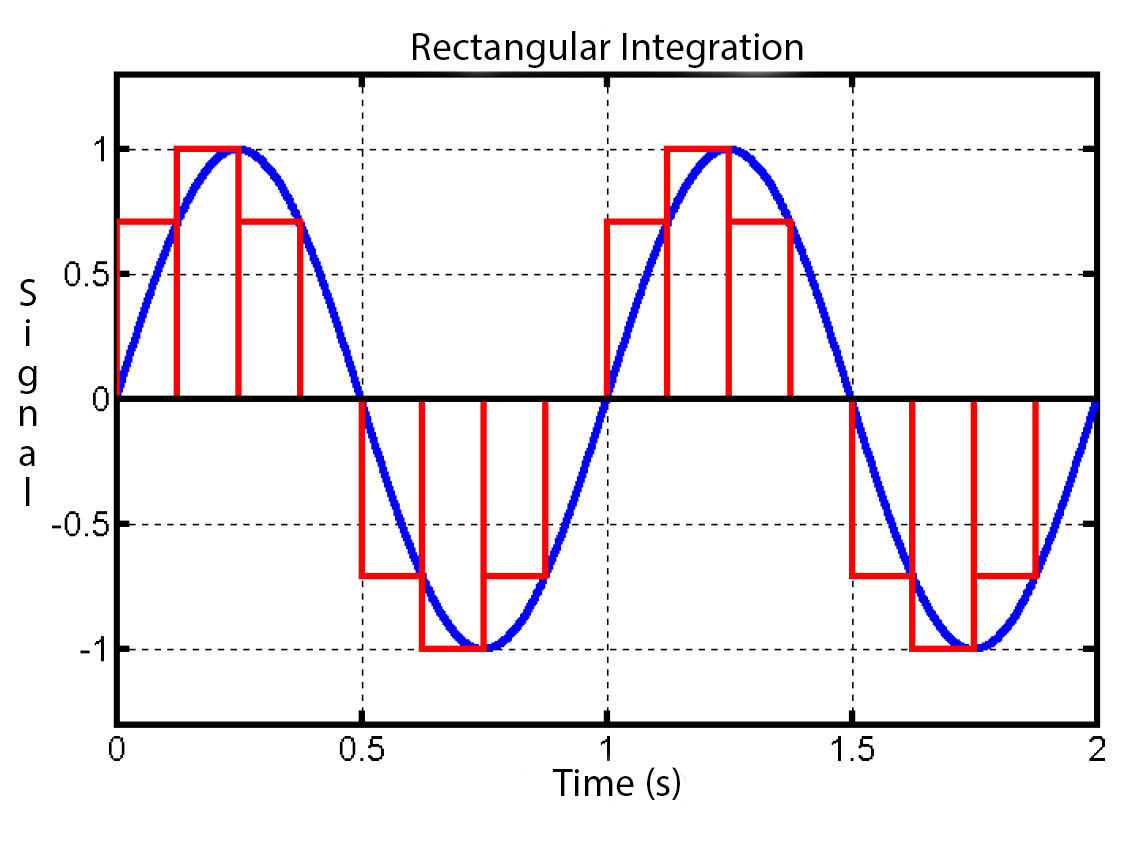
\includegraphics[scale=0.55]{RectangularInte}
\hspace{0.5cm}
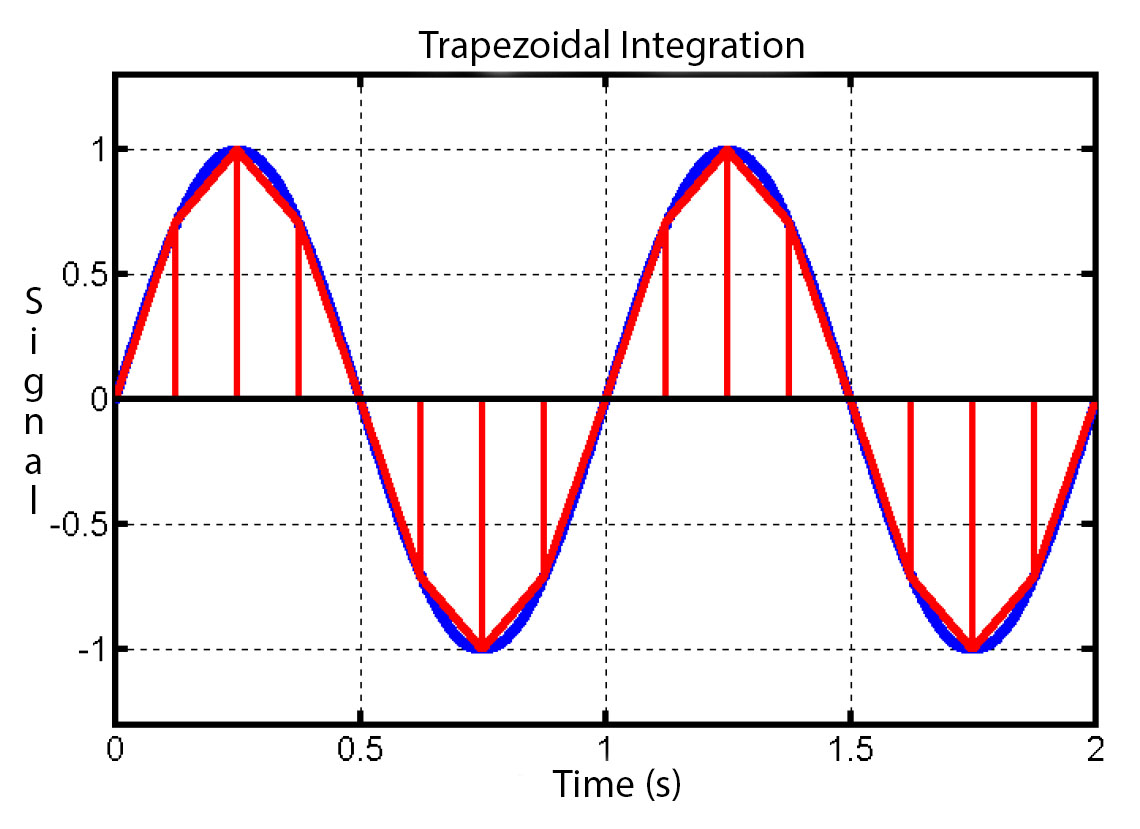
\includegraphics[scale=0.55]{TrapezoidalIntegration}
\caption{Integration using Rectangular (left) and Trapezoidal (right) methods of Sine Wave.}
\label{fig:Rectangular and Trapezoidal Integration}
\end{figure}

The integration was carried out using the trapezoidal method by the MATLAB suite. But without adequate filtering of the signal, the result presents a very error, caused by the drift and noise. 

Various signal filtering procedures will be discussed. The figure below shows the result of a raw signal integration using the  trapezoidal method.

\begin{figure}[H]
  \centering
  \subfloat[Acceleration]{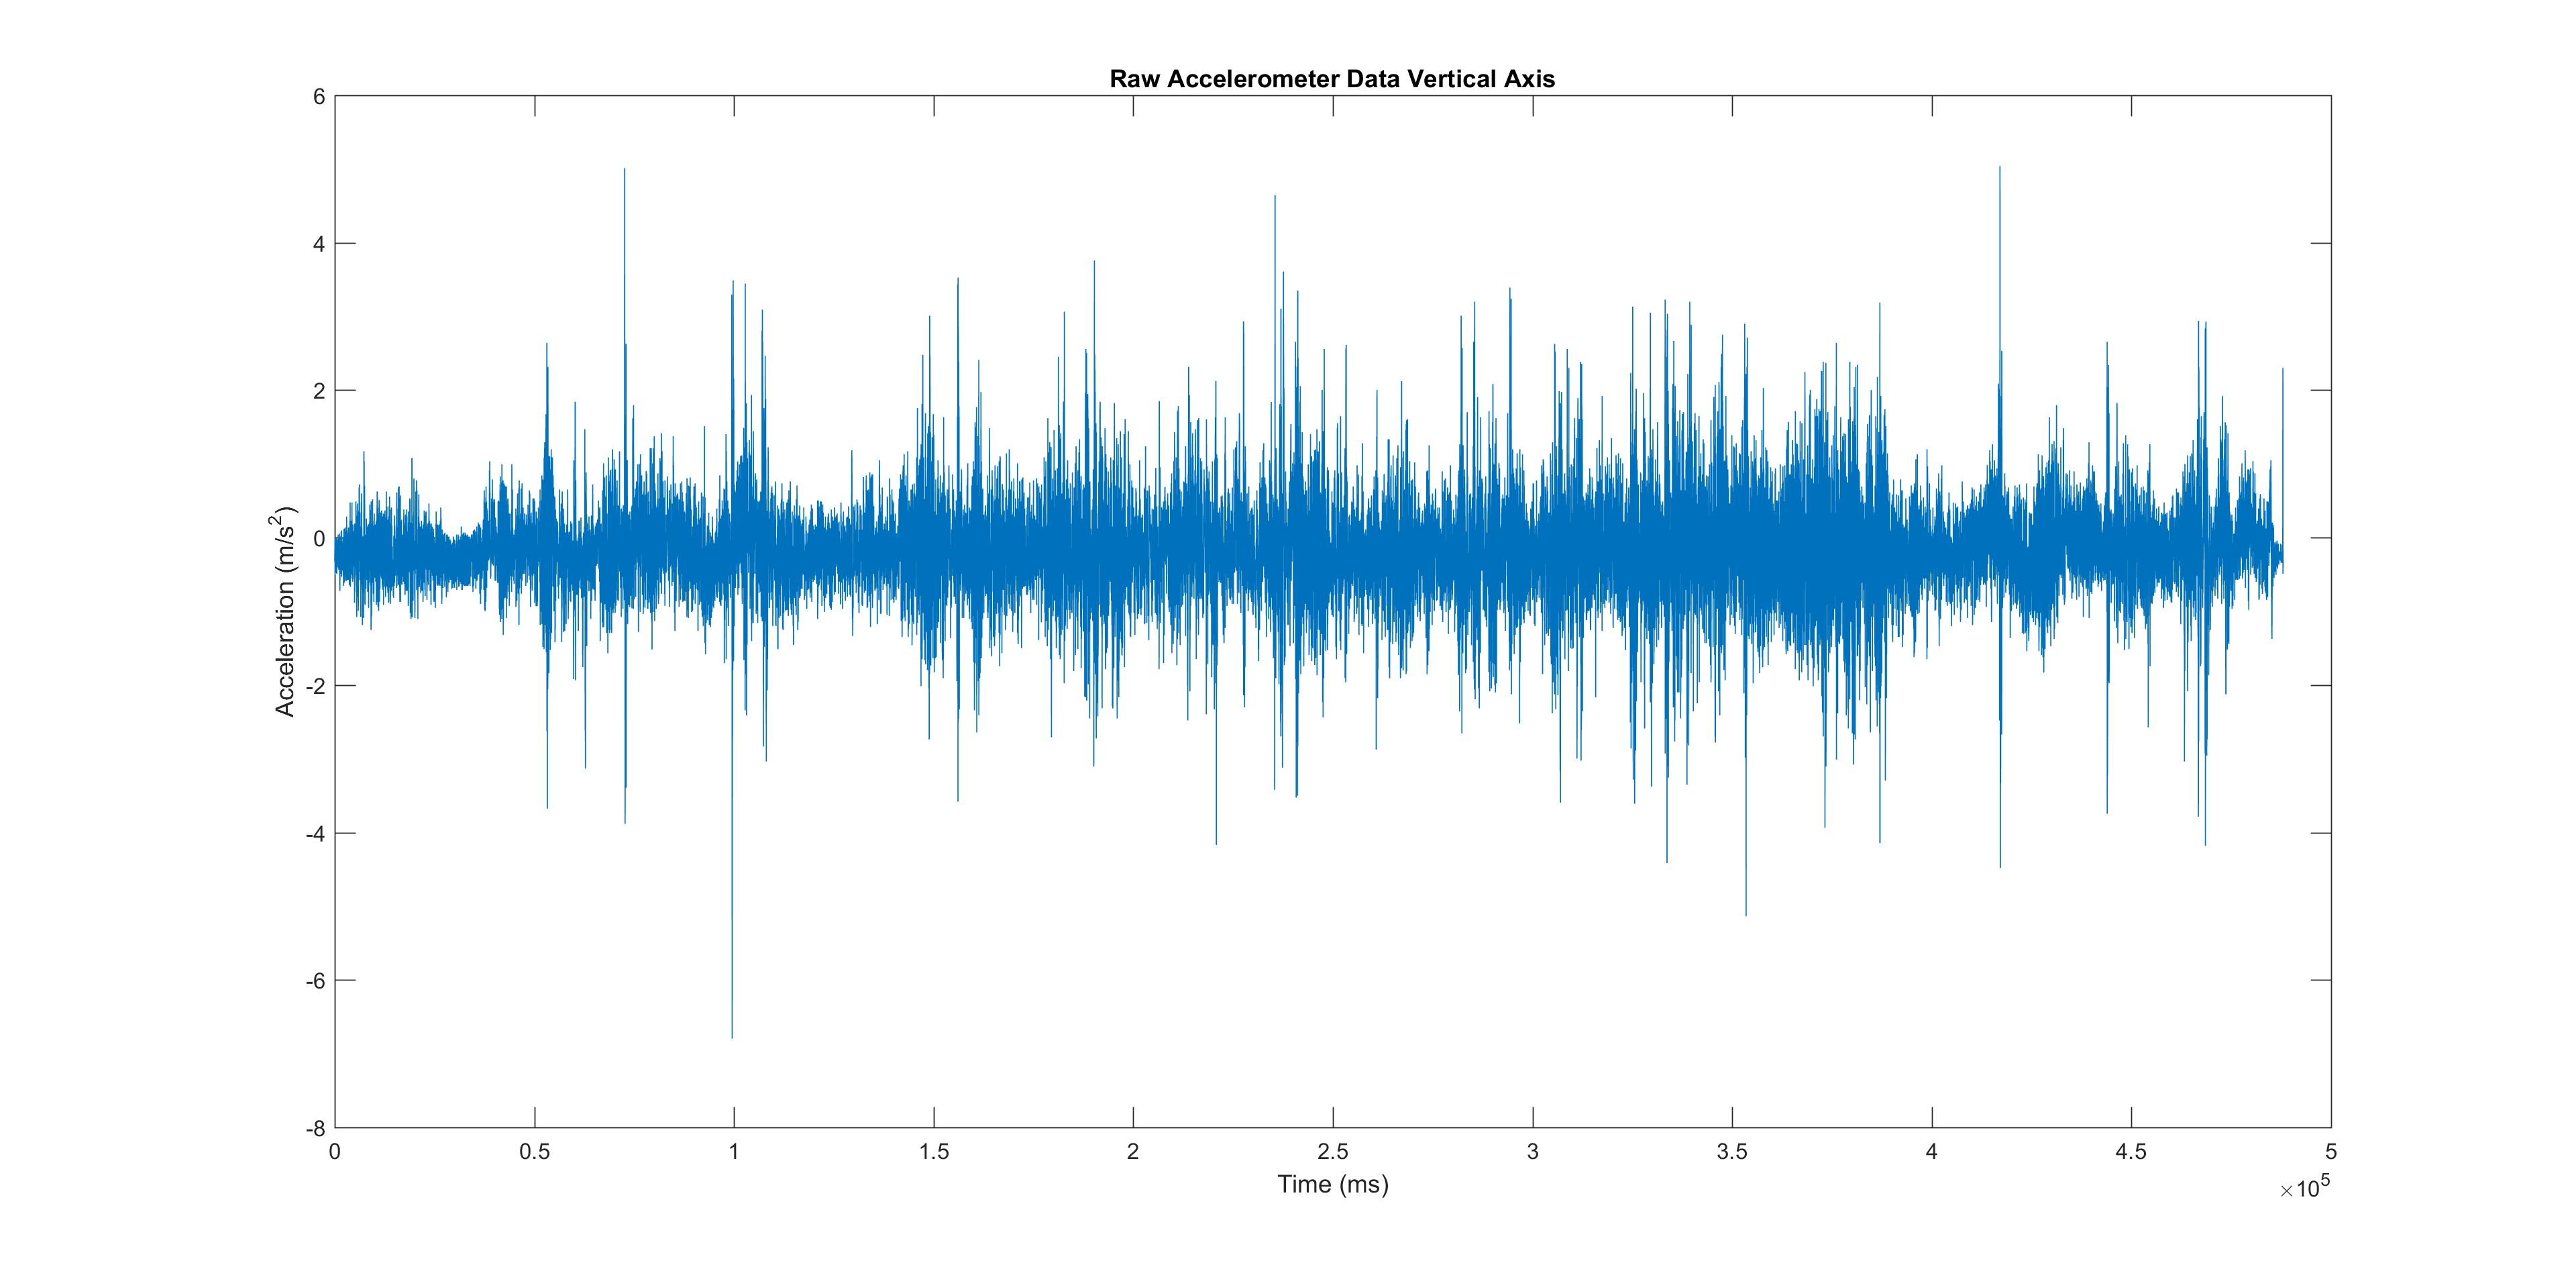
\includegraphics[scale=0.11]{RawAccelerometer}\label{fig:Raw Accelerometer}}  
  
  \subfloat[Velocity]{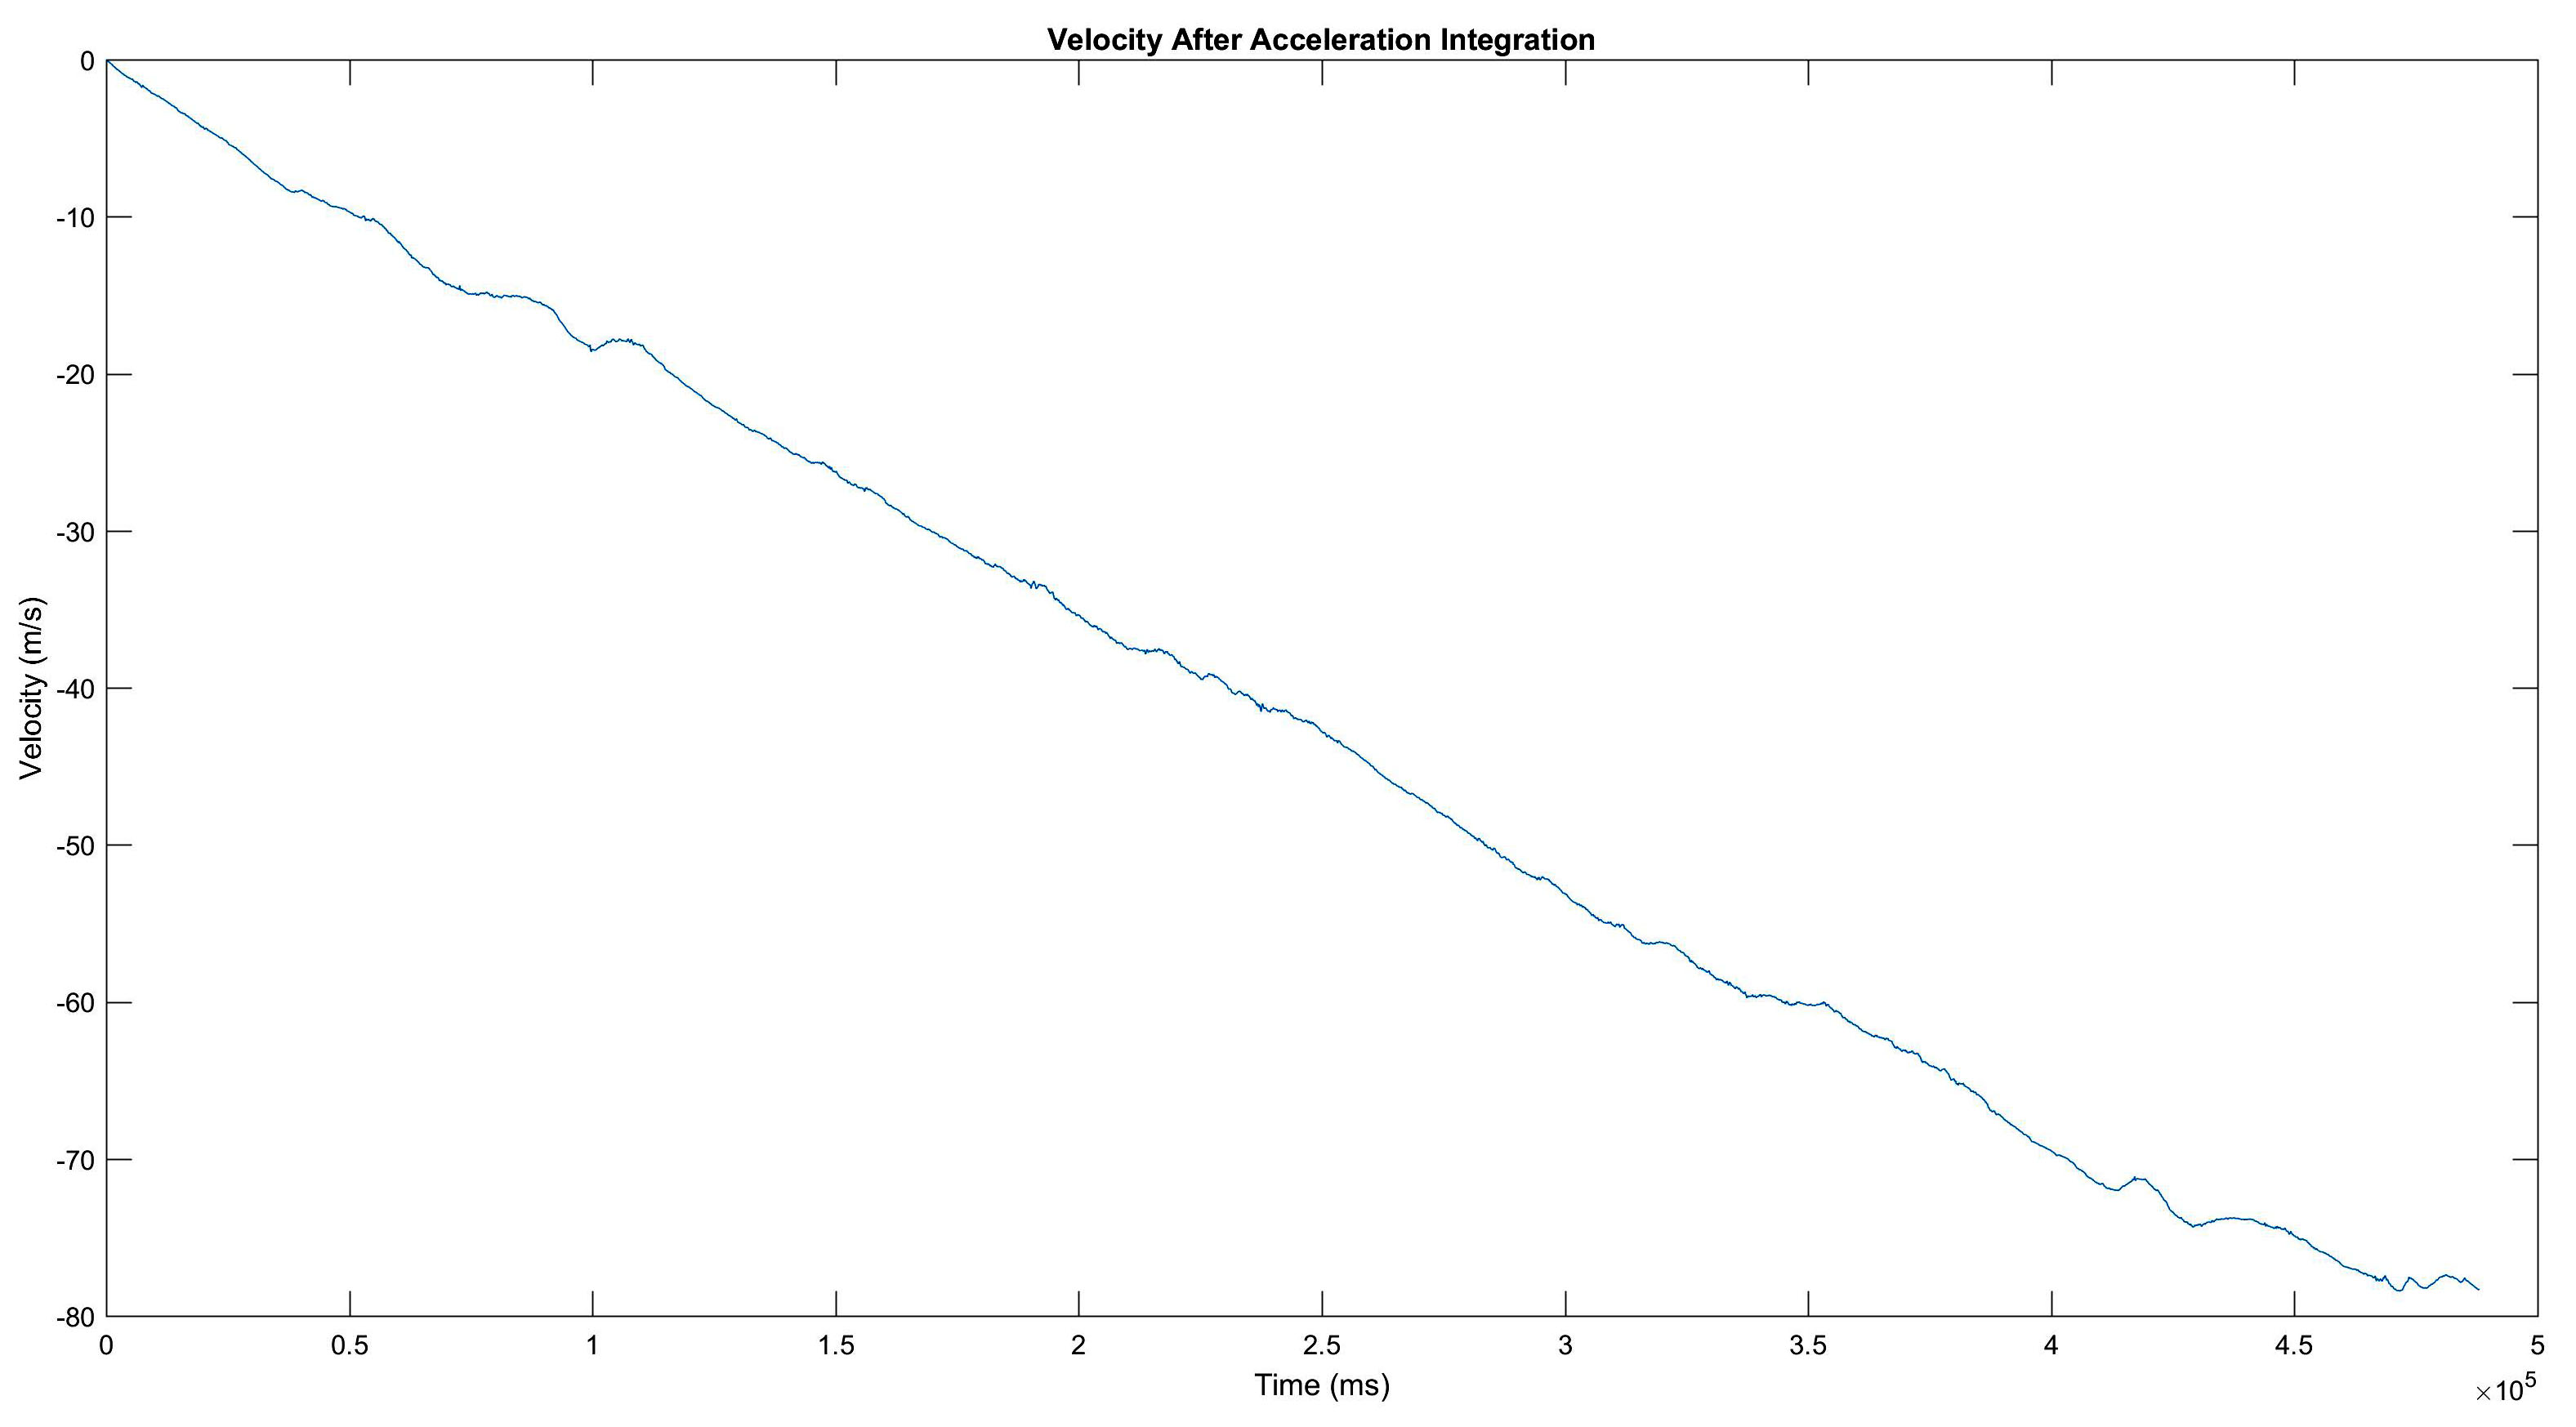
\includegraphics[scale=0.11]{velocityIntegration}\label{fig:Velocity}}

  \subfloat[Displacement]{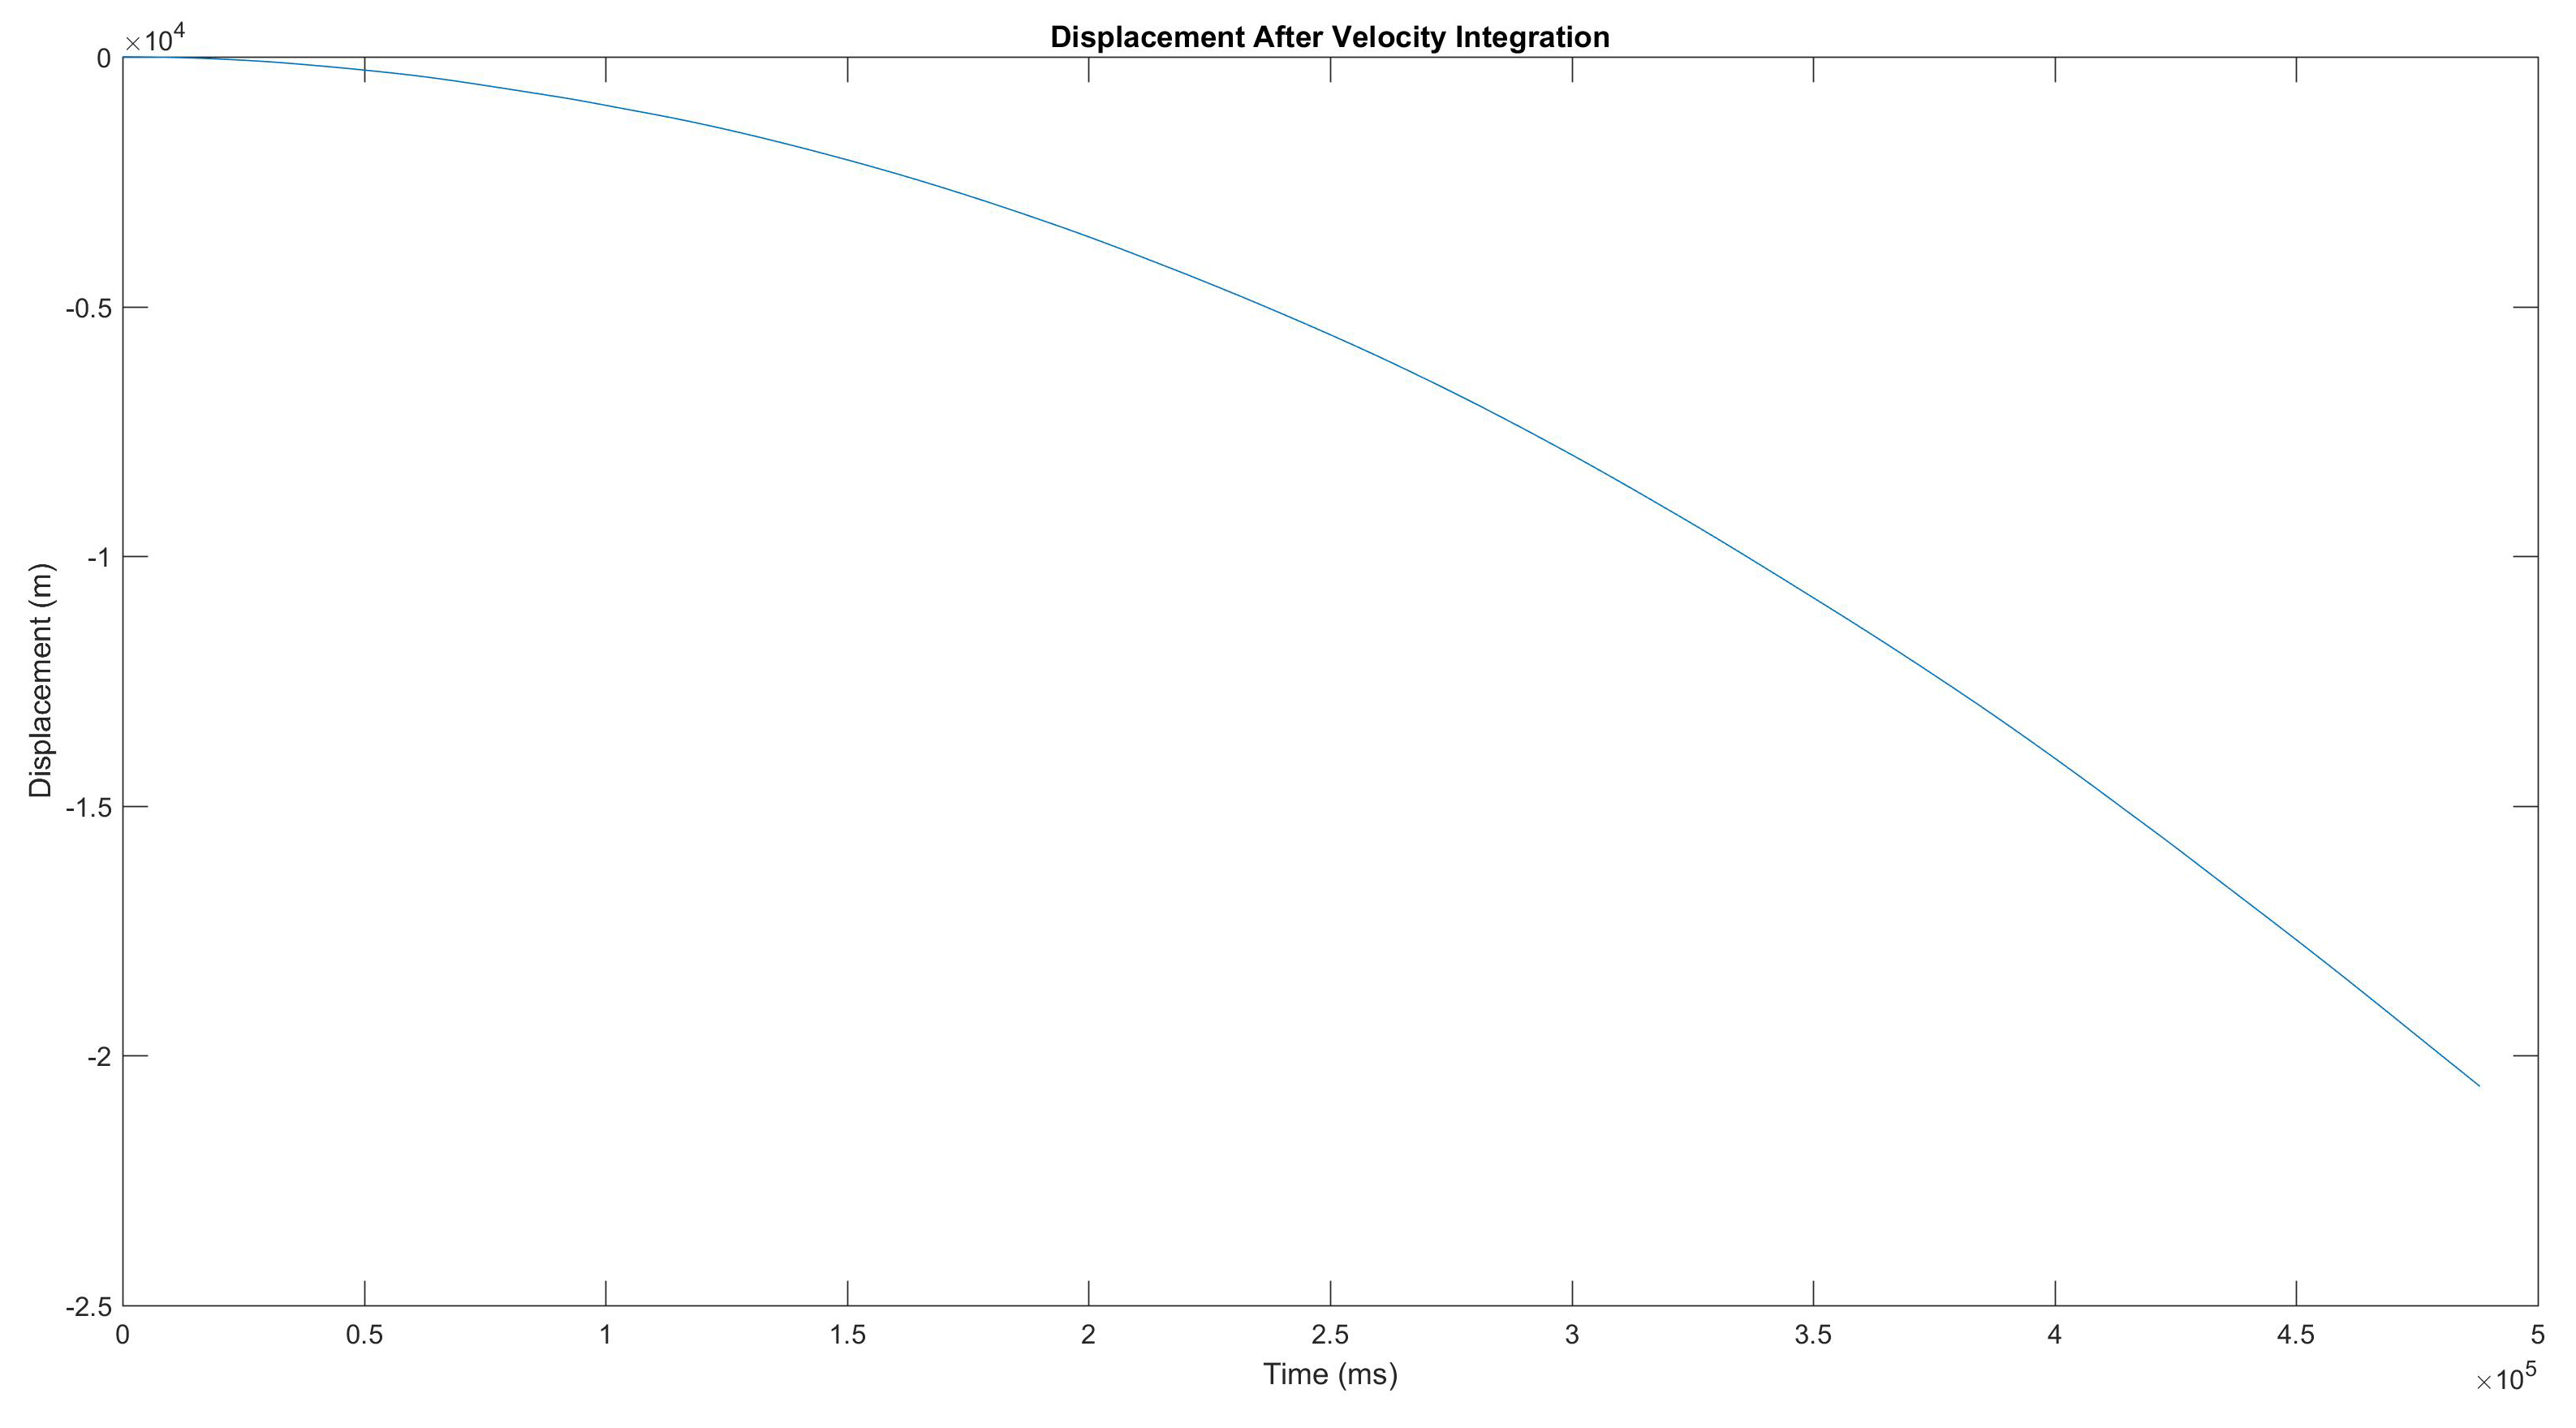
\includegraphics[scale=0.11]{DisplacementIntegration}\label{fig:Displacement}}  
  \caption{The result of double integration of a Raw Signal}
  \label{fig:Integration of Raw Data}
\end{figure}

As is possible see, the result is not realistic, considering it is vertical acceleration, so it is necessary to perform various steps to filter the signal. First of all, the signal reorientation will be carried out respect the axes of the vehicle, and subsequently, various filter operations to smooth the signal.

\section{Accelerometer Reorientation} \label{sc:Accelerometer Reorientation}
The Cartesian reference system of the phone must be aligned with the vehicle reference system, to detect the vehicle motion correctly.
As shown in the figure below.

\begin{figure}[H]
  \centering
  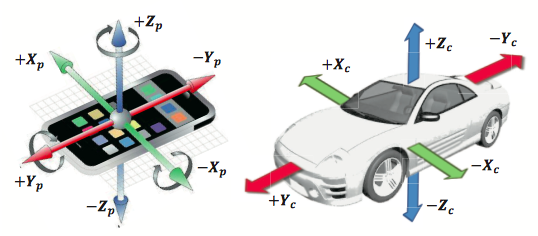
\includegraphics[scale=0.7]{phonecarorientation}  
  \caption{Correct alignment of smartphone respect to the vehicle cartesian frame.}
  \label{fig:Smartphone cartesian frame alignment respect Car axis.}
\end{figure}
\noindent Smartphone accelerometer detects the following accelerations: $a_{x_{p}}$ , $a_{y_{p}}$ and $a_{z_{p}}$ . To determine the accelerations felt by the vehicle and locate road surface anomalies. The accelerometer must detect what happens in the direction perpendicular ($Z$ axes) to the vehicle\cite{mohan2008nericell}.
Respectively the $X_{p}$ axis identifies the longitudinal direction, $Y_{p}$ axis the transverse direction and $Z_{p}$ the perpendicular direction respect to the $xy$ plane.

\vspace{0.25cm}
To detect road anomalies, the direction of the z-axis must correspond to the direction of the z-axes. If this condition subsists, the accelerometer is well oriented, contrarily it is not well oriented and needs to be reoriented. But even if starting from a precise orientation condition, during travel the phone may be moving, or due to unexpected vehicle movements, travel of climbing, downhill, curve, all of these causes could affect the misalignment of the smartphone frame respect to the vehicle frame.
\clearpage
The reorientation can be performed by the Euler Angles. Three angles that allow to defining the orientation in space of any body through a succession of elementary rotations\cite{diebel2006representing}.
The $XYZ$ sequence was defined, a rotation around the $x$-axis by an angle $\alpha$ (roll angle), one around the $y$-axis by $\beta$ (pitch angle) and one around the $z$-axis by  $\gamma$ (yaw angle).
\noindent The equations that allows to reoriented data by the $\alpha$, $\beta$, $\gamma$, angle are:\cite{Andro}
\begin{equation}
a_{x_{reor}} = \cos (\beta) a_{x_{p}} + \sin (\beta) \sin (\alpha) a_{y_{p}} + \cos (\alpha) \sin (\beta) a_{z_{p}} 
\end{equation}
\begin{equation}
a_{y_{reor}} = \cos (\alpha) a_{y_{p}} - \sin (\alpha) a_{z_{p}}
\end{equation}
\begin{equation}
a_{z_{reor}} = -\sin (\beta) a_{x_{p}} + \cos (\beta) \sin (\alpha) a_{y_{p}} + \cos (\beta) \cos (\alpha) a_{z_{p}}
\end{equation}


\noindent The figure below, show an example of reoriented data.
\begin{figure}[H]
  \centering
  \subfloat[Raw]{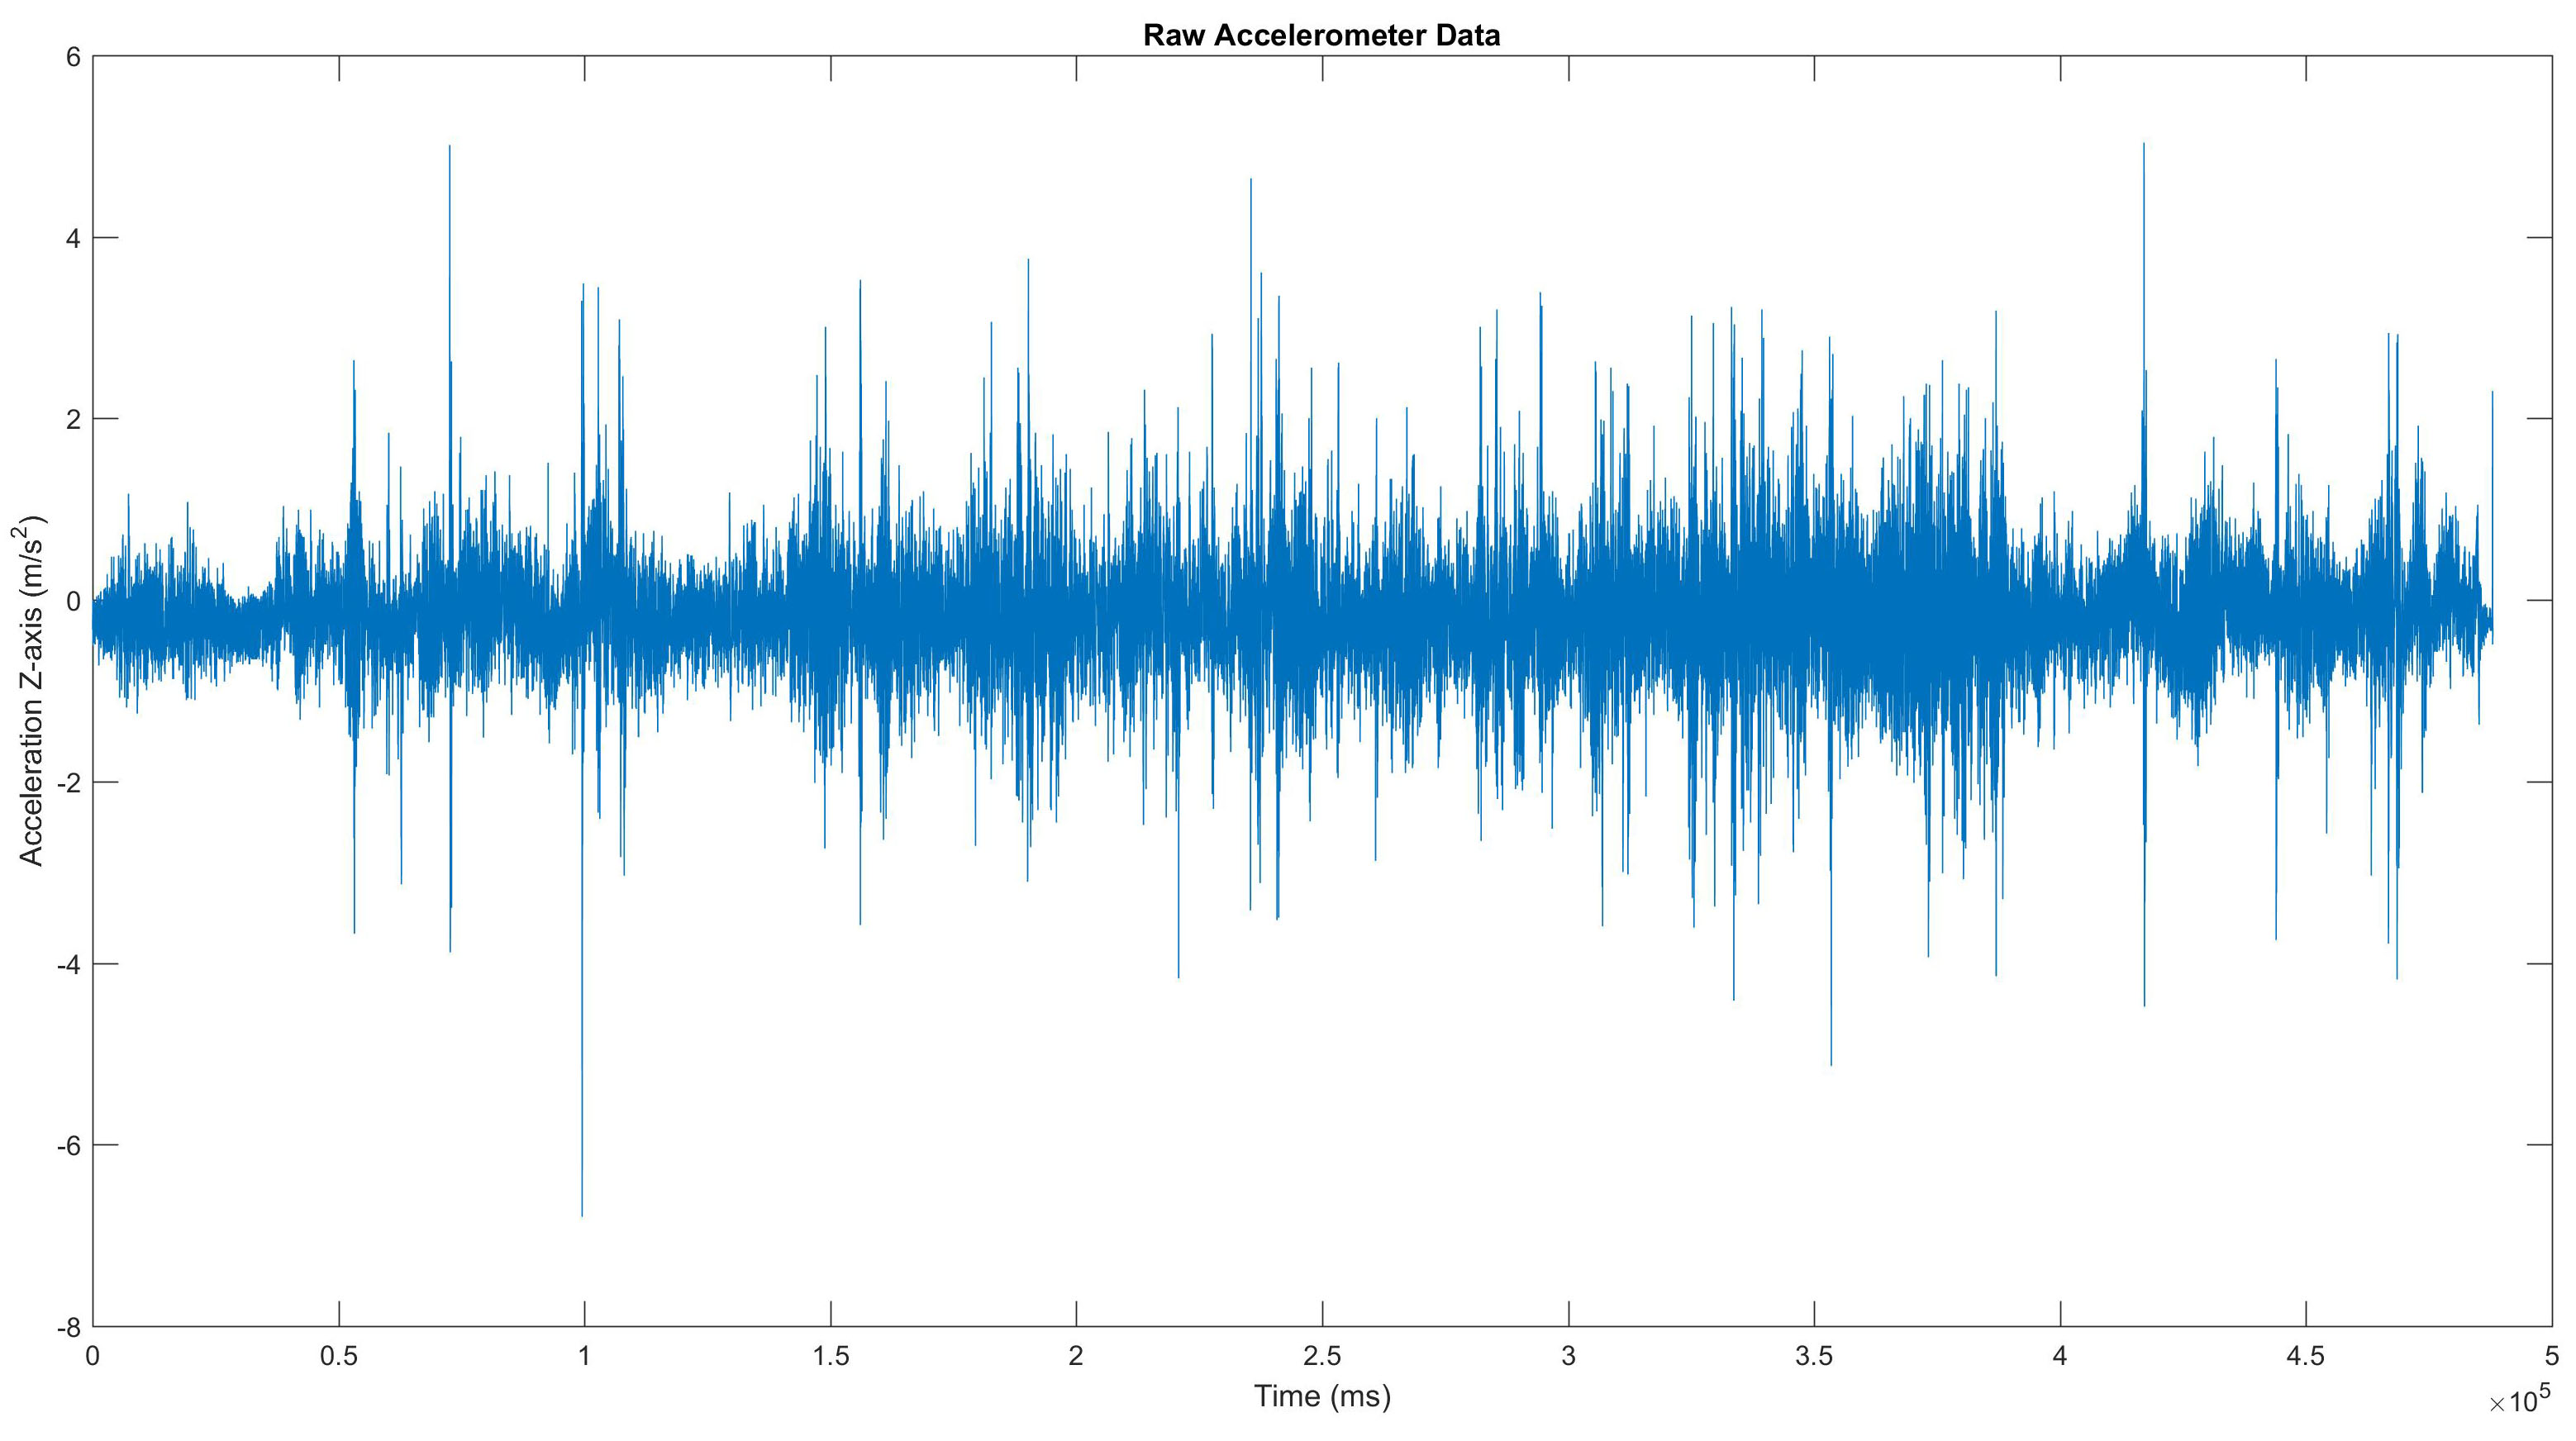
\includegraphics[scale=0.11]{raw}\label{fig:Raw Accelerometers}}  
  
  \subfloat[Reoriented]{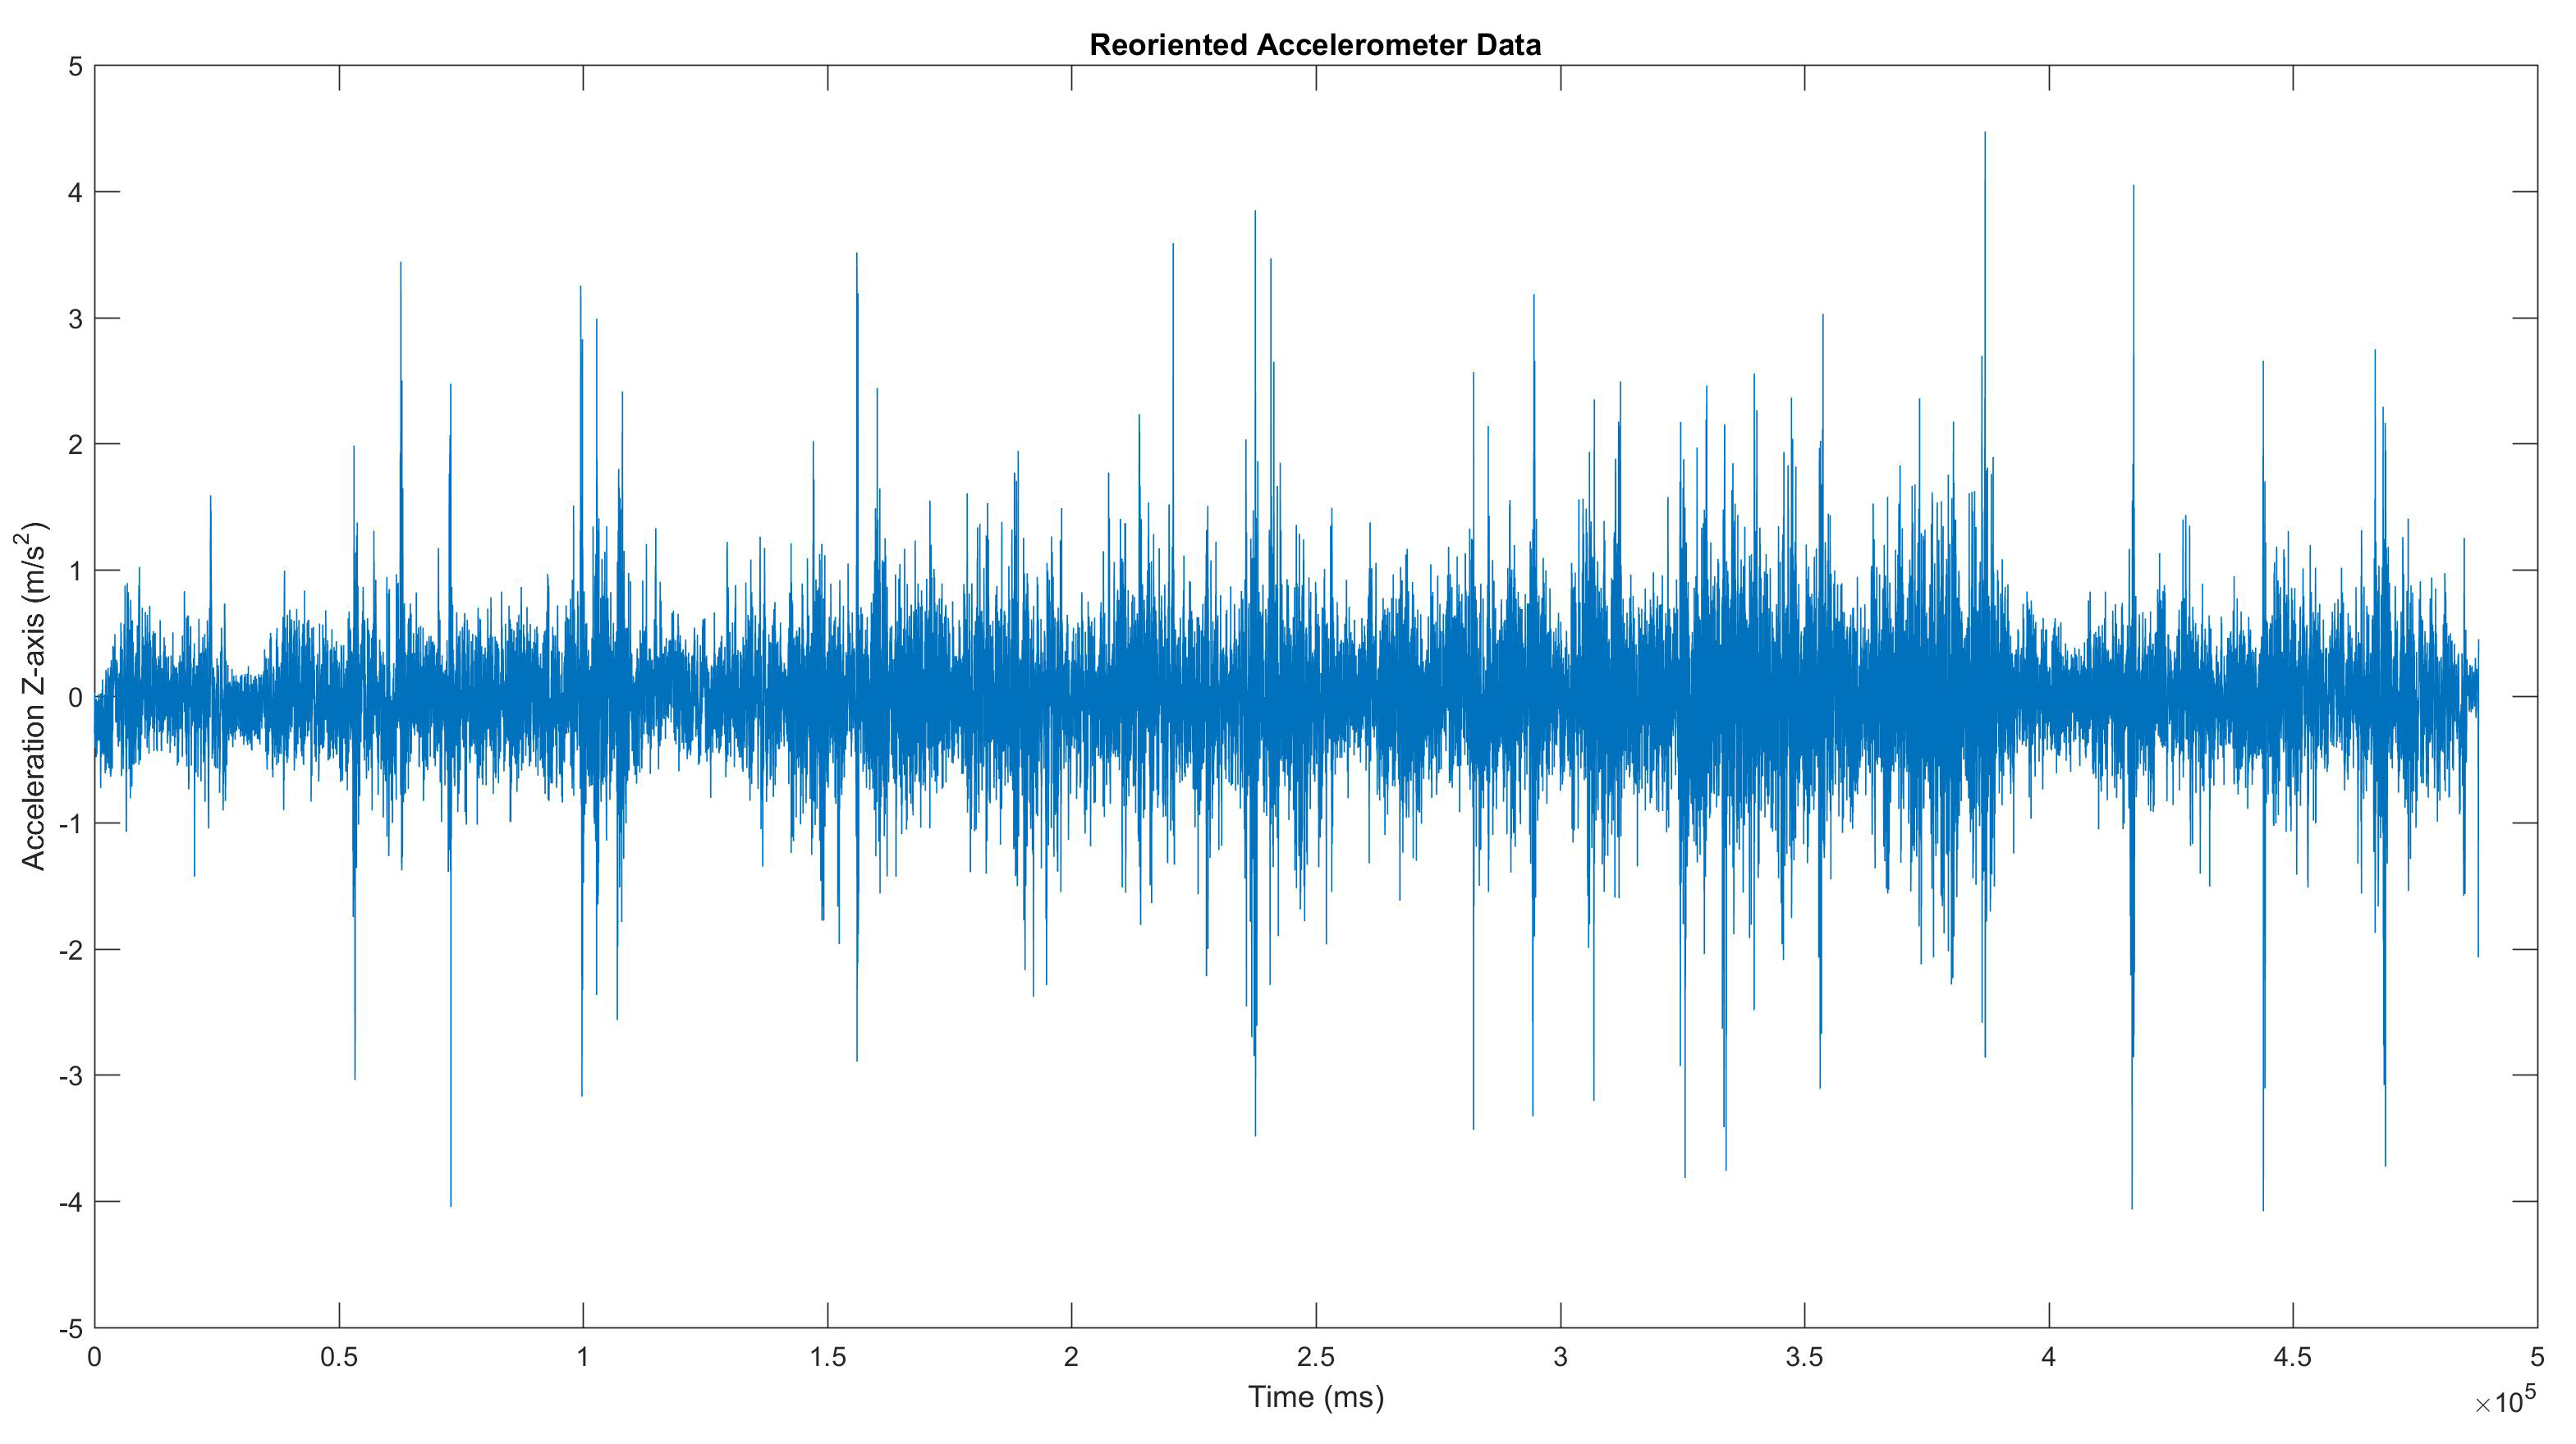
\includegraphics[scale=0.11]{reoriented}\label{fig:Reoriented Accelerometer}}

 
  \caption{The result of reorientation of raw data}
  \label{fig:Accelerometer Reoriented}
\end{figure}

\section{Data Filtering} \label{sc:Data Filtering}
As can be seen in figure \ref{fig:Integration of Raw Data}, a data filtering operation is needed to smooth the signal and perform a better integration.
It is necessary to apply:

\begin{itemize}
\item A series of preliminary filters for removing unimportant information.
\item A digital filter for removing certain frequency components that cause the error at the stage of integration.
\end{itemize}



\subsection{Preliminary Filtering}\label{ssc:Preliminary Filtering}
During signal capture, it is important to consider some information that can be removed, since they are not relevant to the final calculation. These principal regard:
\begin{itemize}
\item The background noise generated by engine vibrations.
\item Acceleration components recorded at the moment the vehicle is stationary, so when its velocity is equal to $0$ $\si{\km\per\hour}$.
\end{itemize}

\noindent These two filters are applied to all three indexes (IRI, Critical Points, Simple Acceleration Points) that are extrapolated from the data series.

\subsubsection{Filtering Engine Vibrations} \label{sssc:Remove Engine Vibrations Filter}
Considering the vehicle in a stationary position, both flat, uphill and downhill, with no any external form of acceleration given by the pilot, so at no speed. Many measurements have been made to see how much the engine vibration affects the process of data acquisition.
Analyzing these measurements, two thresholds, one minimum and one maximum were identified, called respectively \textbf{$a_{min_{th}}$} and \textbf{$a_{max_{th}}$}.
Next, considering the generic acceleration signal at time $a_{t}$, the data series is thus modified:


\begin{center}
\[
    \left\{
                \begin{array}{ll}
                  a_{t} = a_{t} - a_{max_{th}}; \quad 	if \quad a_{t} > a_{max_{th}}\\
              	  a_{t} = a_{t} + |a_{min{th}}|; \quad  if \quad a_{t} < a_{min_{th}}
                \end{array}
              \right.
\]
\end{center}
or:
\begin{center}
$a_{t} = \sqrt{\dfrac{1}{k} (a_{t_{i}}^{2} + a_{t_{i+1}}^{2} + ... + a_{t_{i+k}}^{2} )} $\\
\end{center}
\begin{center}
$if\quad  a_{min_{th}} <= a_{t} <= a_{max_{th}} $


Where $k$ is the number of a predefined window, and all the values that fall into the window indexes will be considered.
So the final value $a_{t}$ will be calculated as the Root Mean Square of that values.
\end{center}

The figure below shows an example of applying the filter to a series of data subject only to the reorientation operation\ref{sc:Accelerometer Reorientation}.

\vspace{0.5cm}
\begin{figure}[H]	

\subfloat[Acceleration]{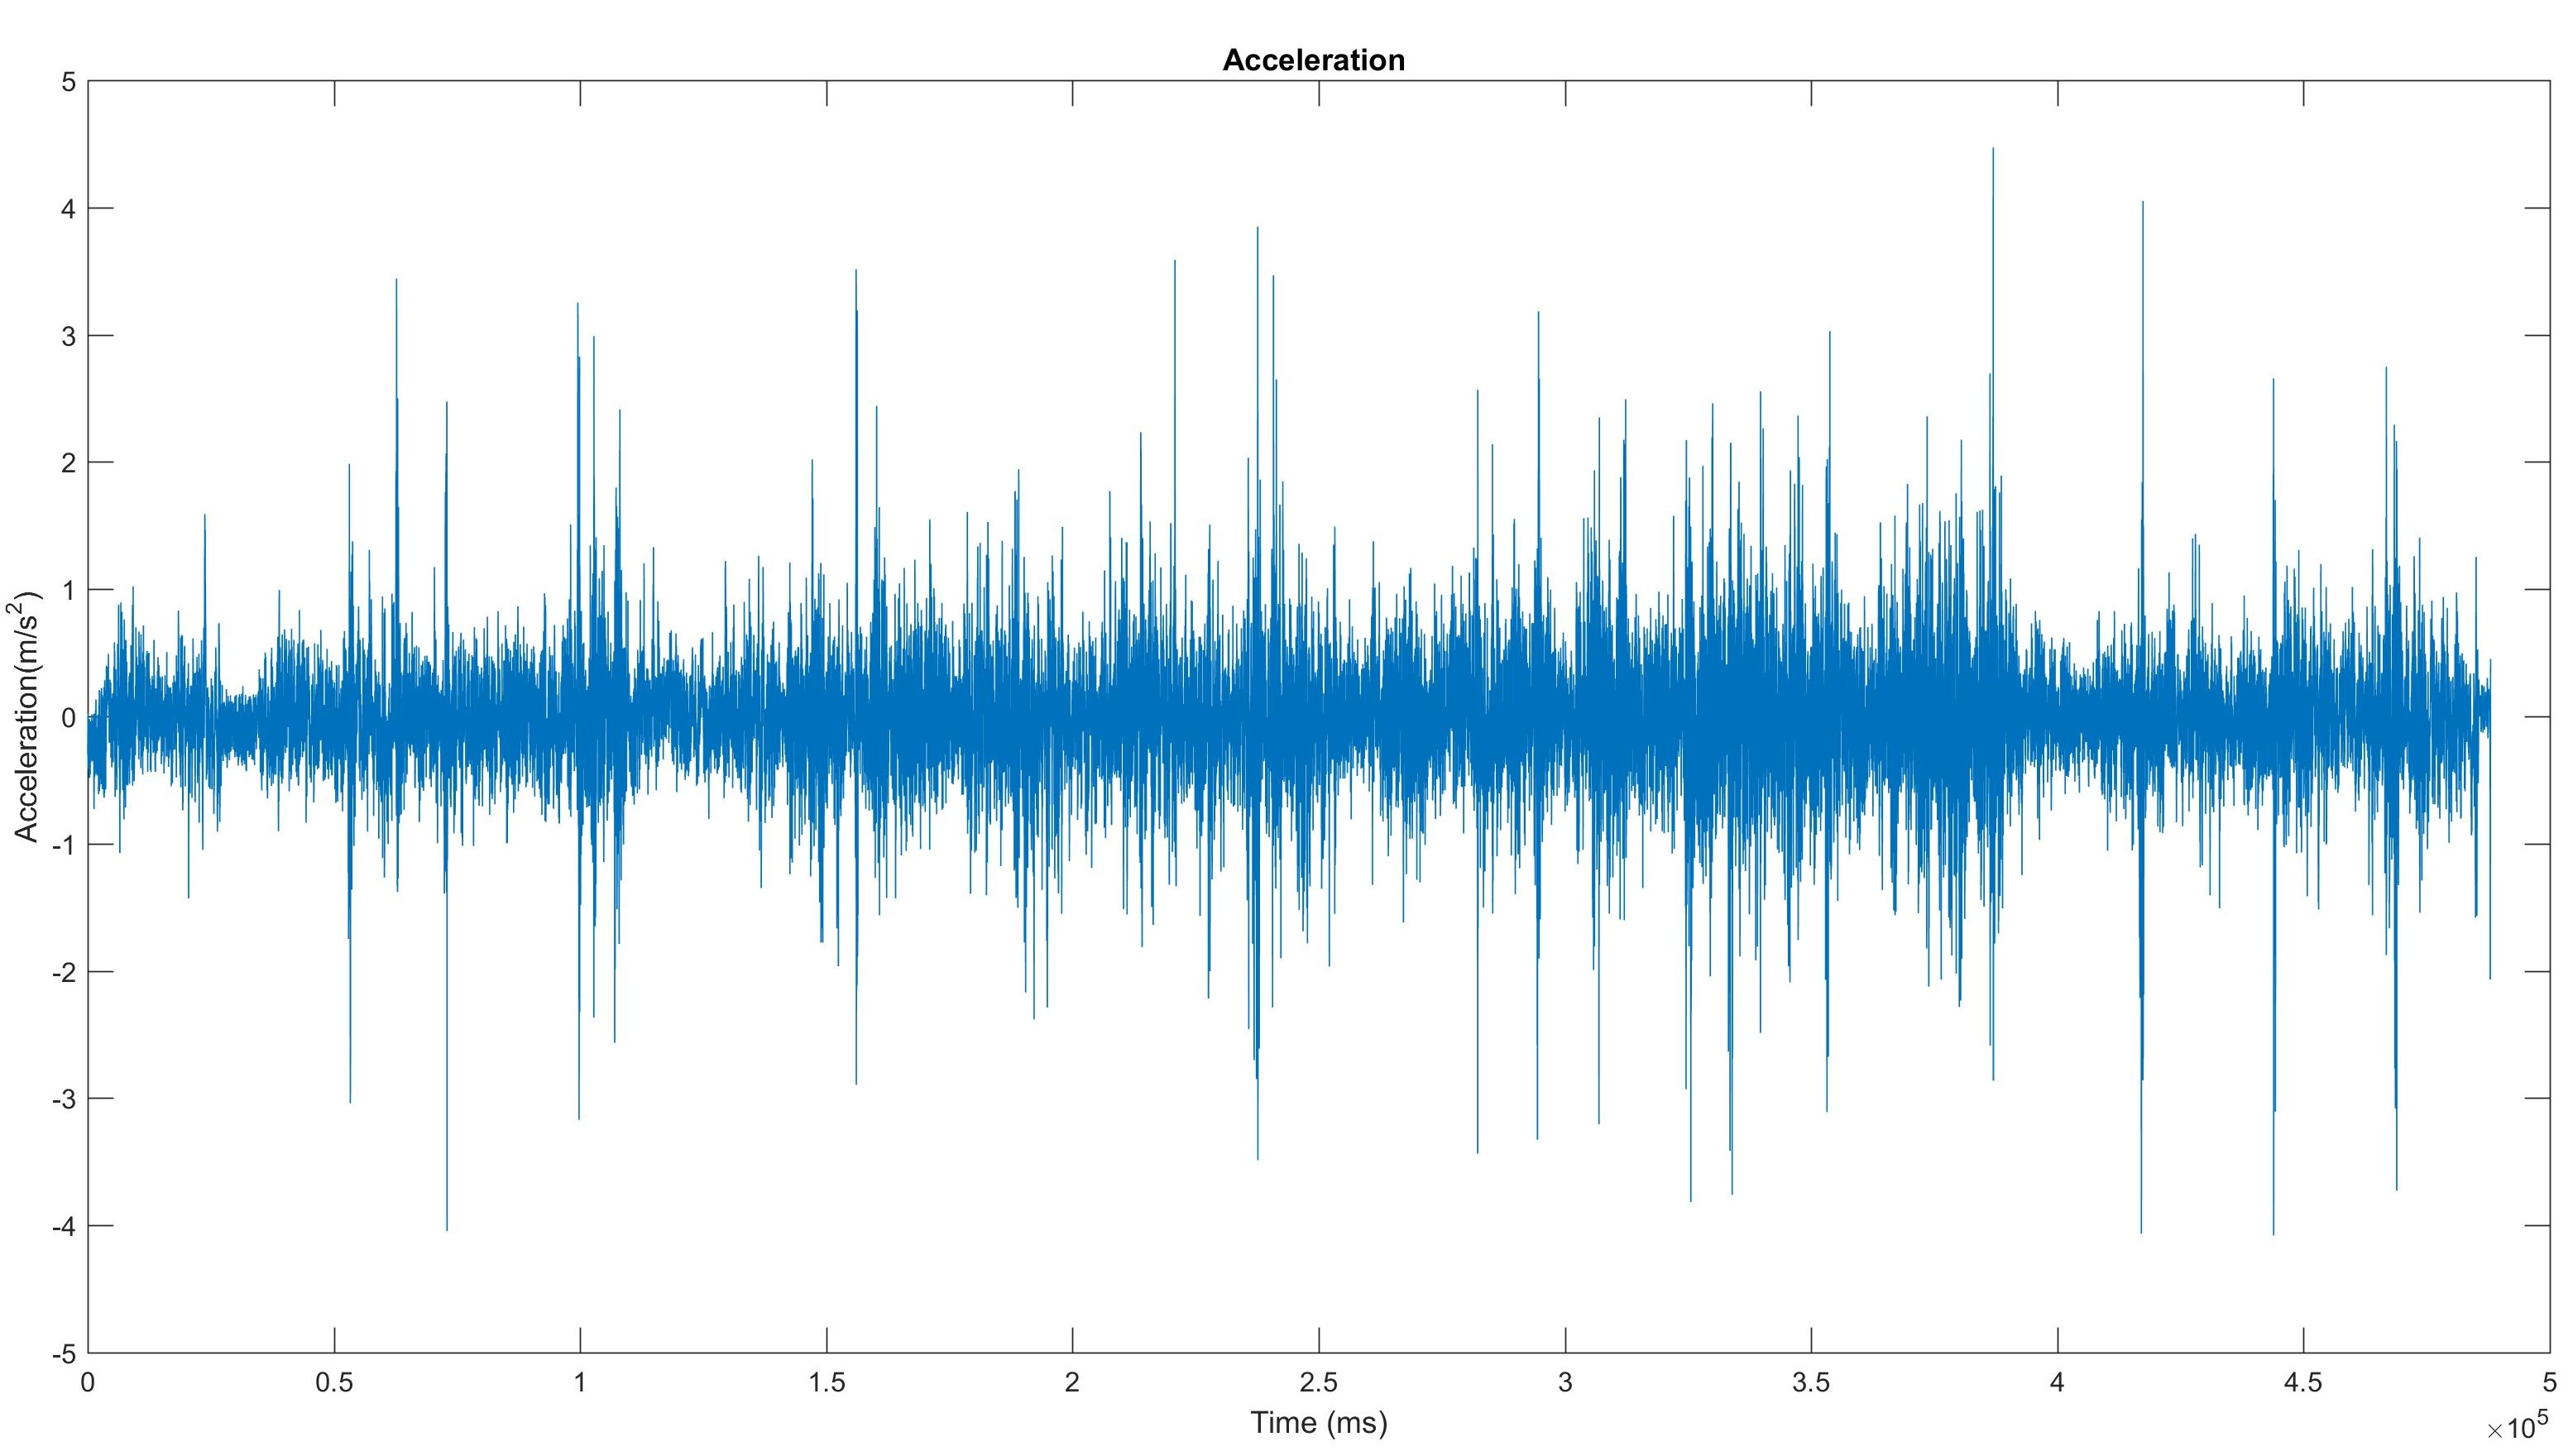
\includegraphics[scale=0.1]{WithRumors}}    
\subfloat[Acceleration after filtering]{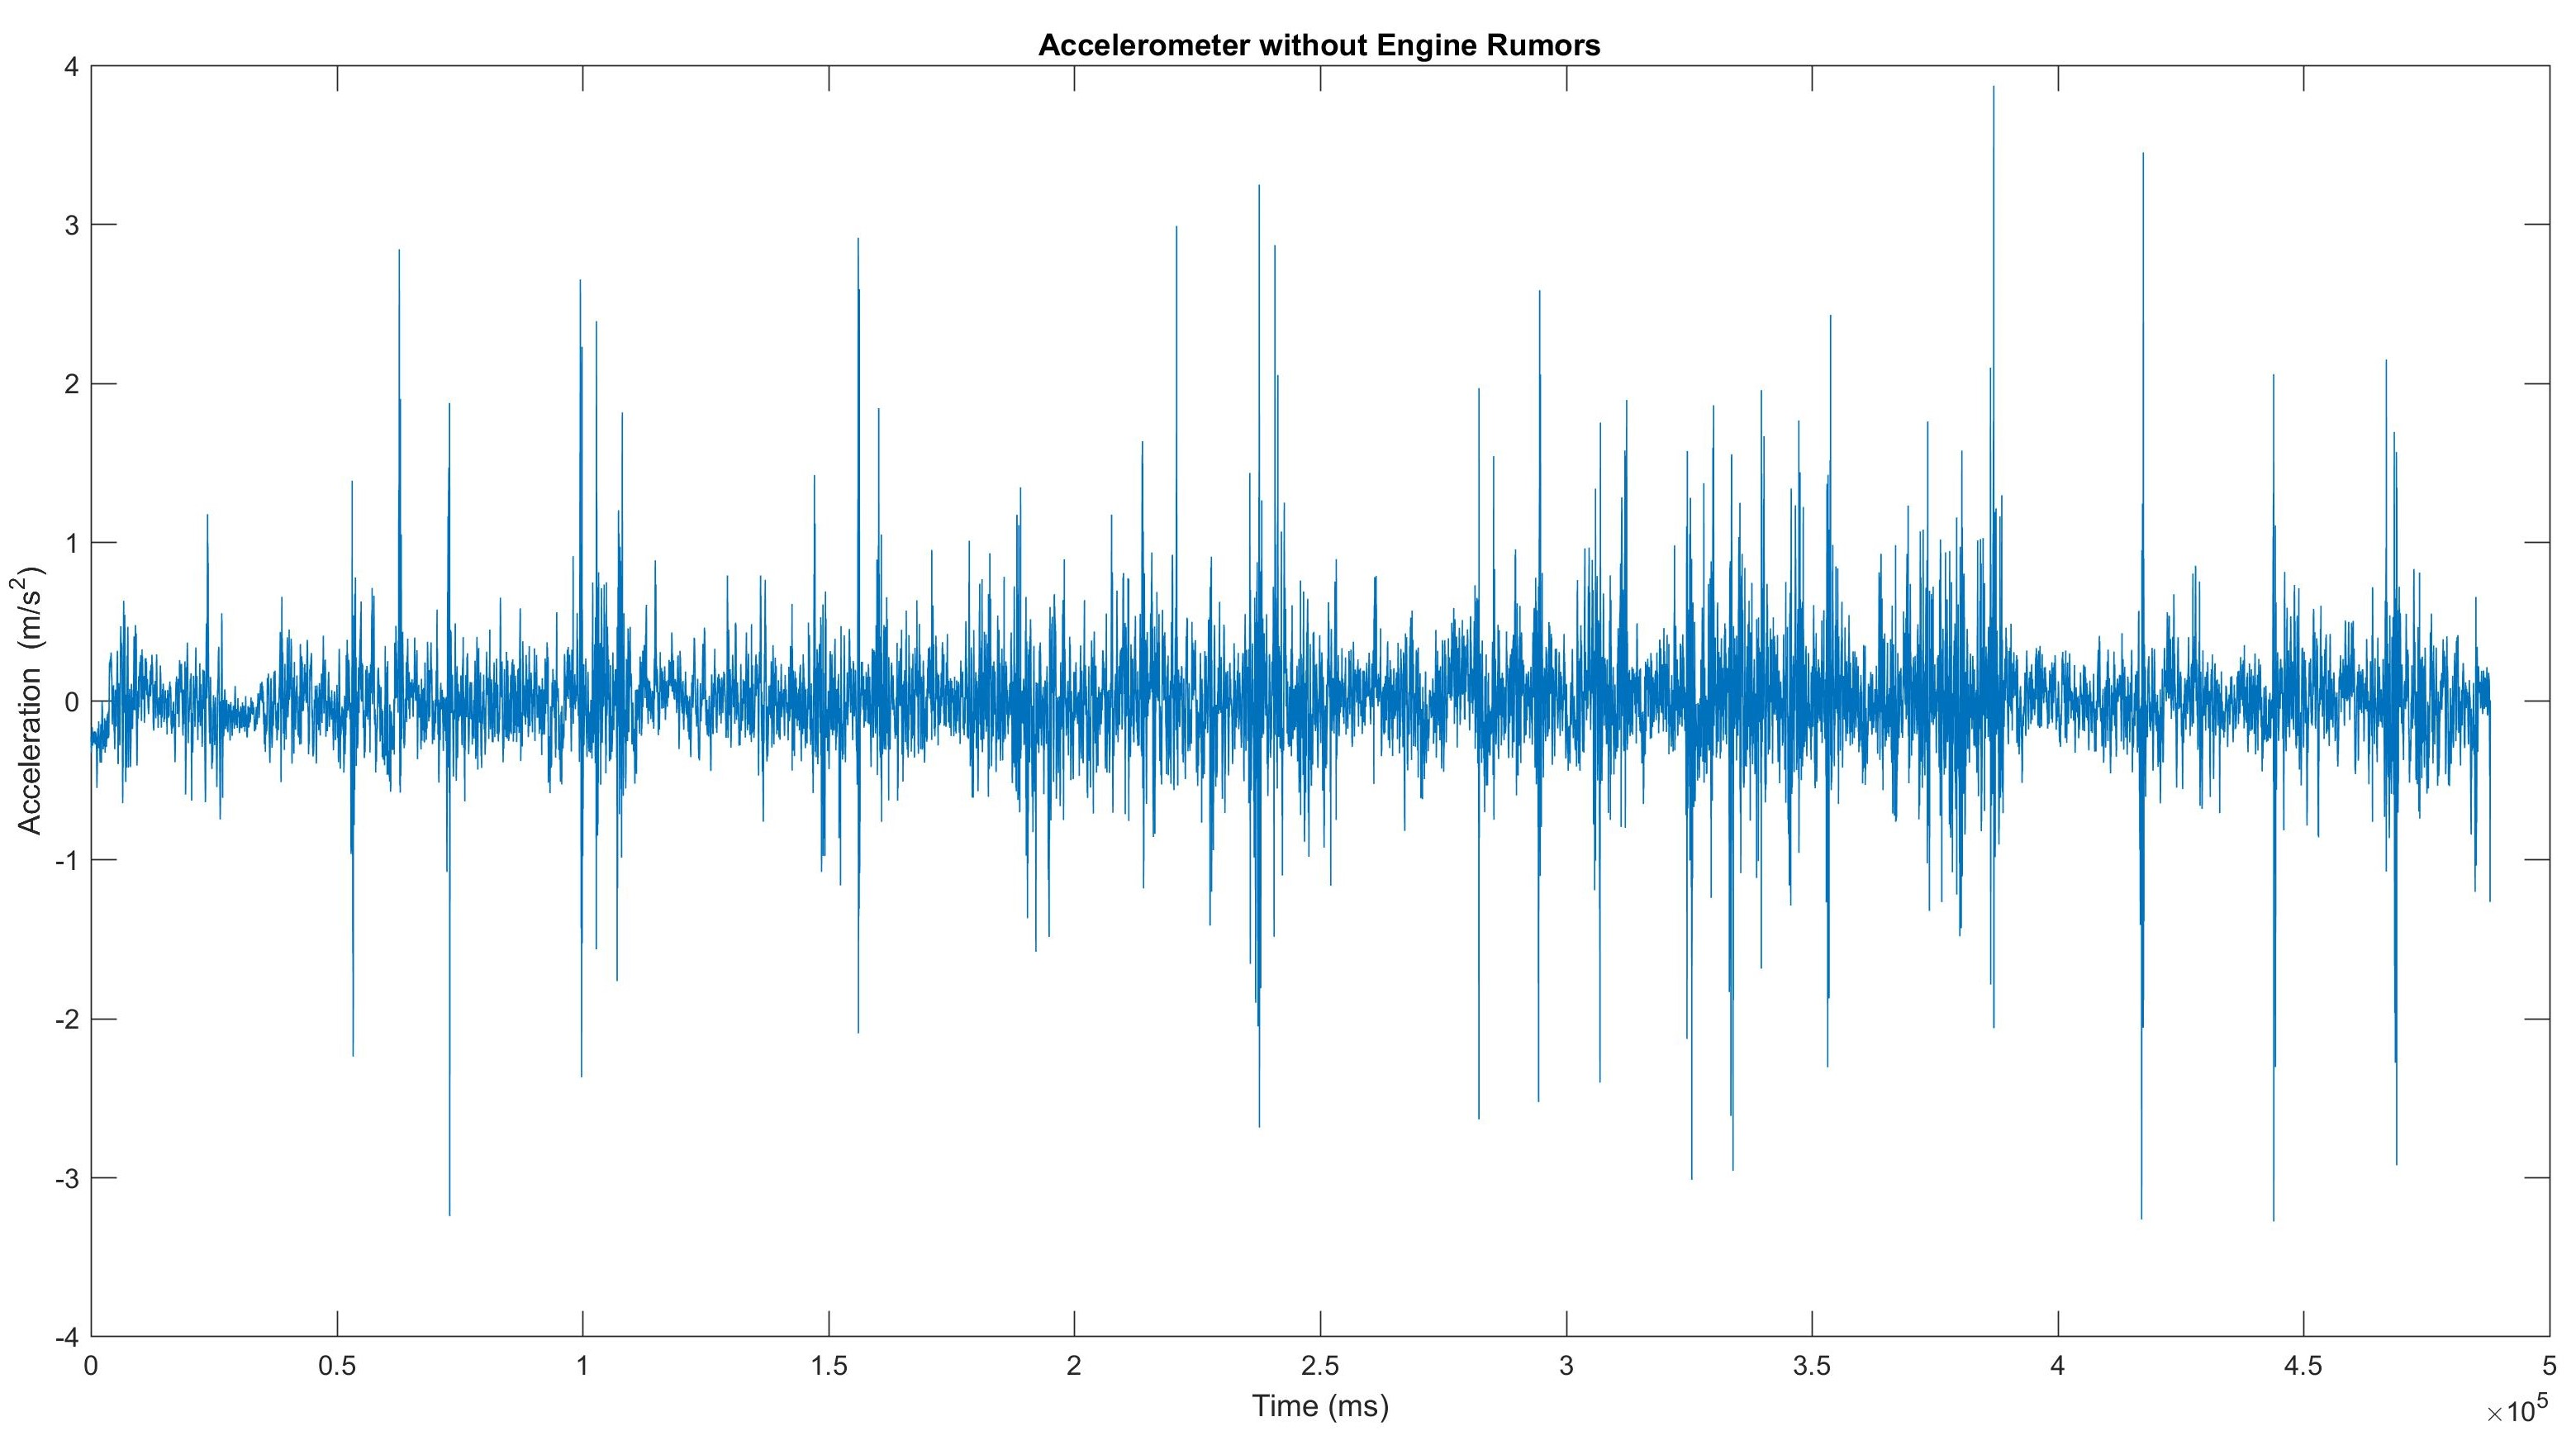
\includegraphics[scale=0.1]{NoRumors}}

\centering
\subfloat[Signal Overlapping]{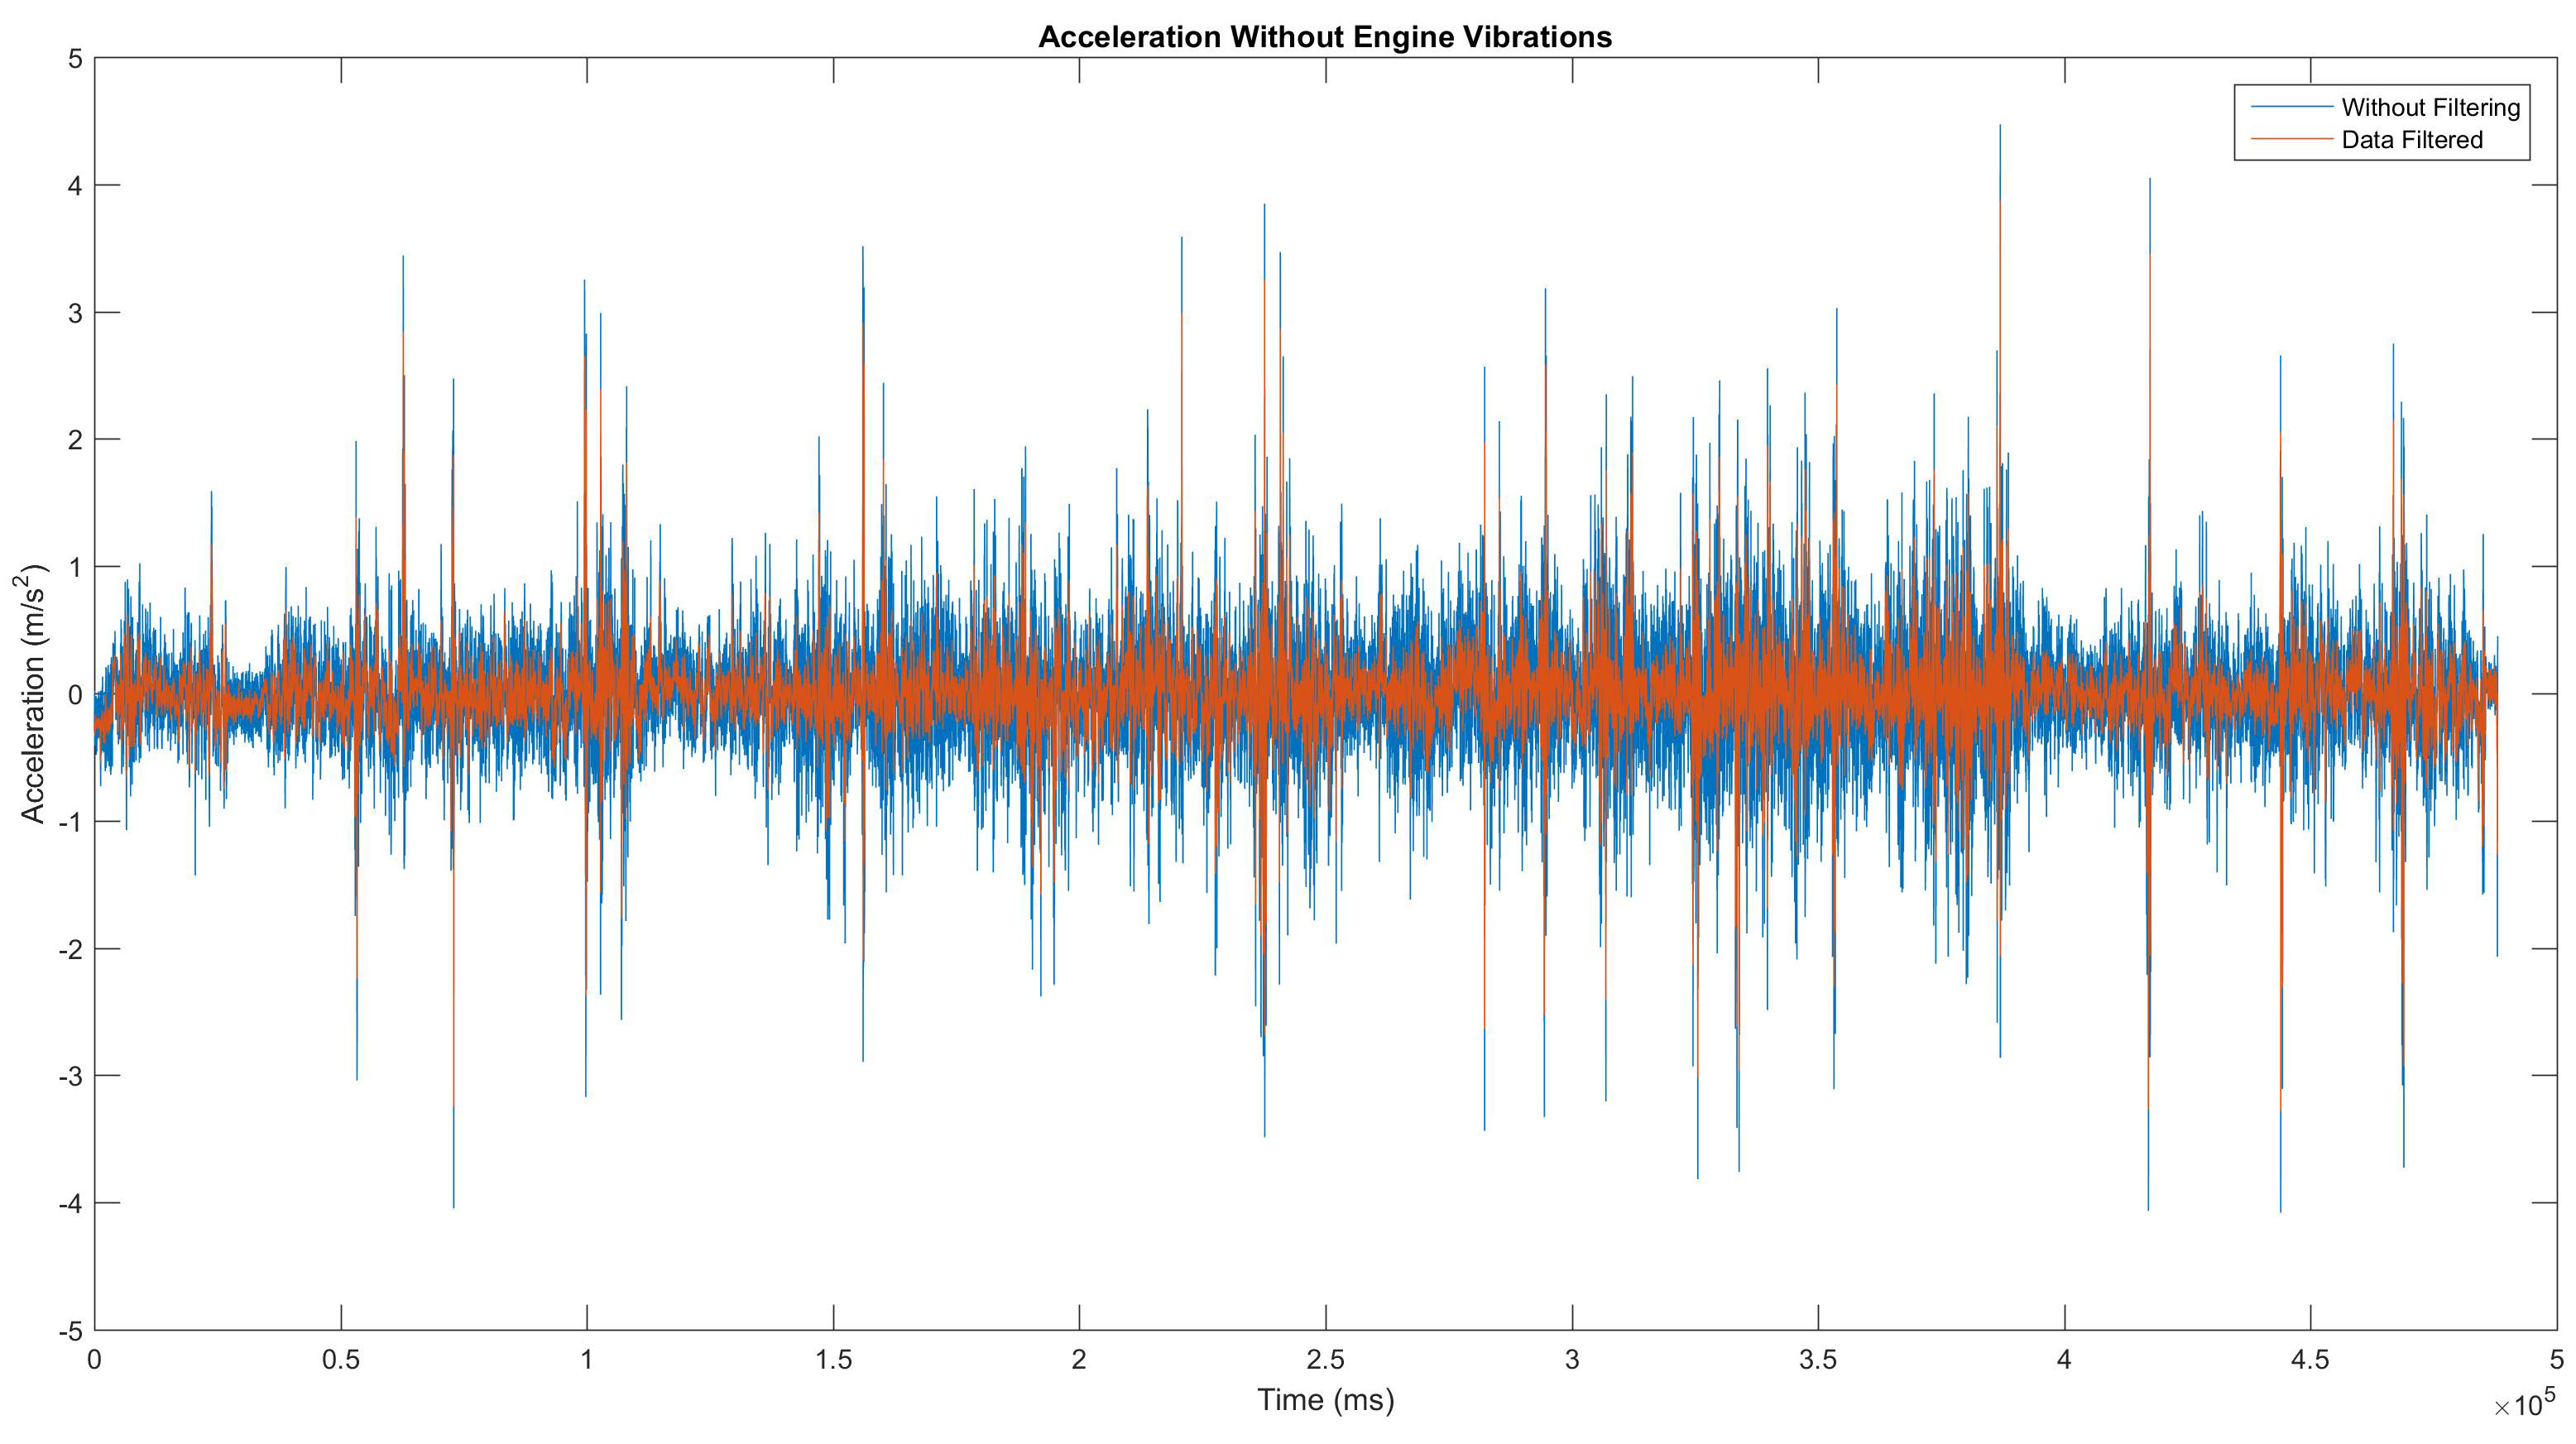
\includegraphics[scale=0.1]{EngineRumors}}

The original signal (a) is represent in blue, the filtered signal is represent in orange (b).
 \caption{Application of Filtering Engine Vibrations}
  \label{fig:Application of Engine Vibrations Filter.}
\end{figure}
As is possible to see the signal when filtered it is much lighter, the background noise component produced by the engine is very resonant during the acquisition process and with this process it is possible to delete it.

\subsubsection{Zero Velocity Filter}\label{sssc:Zero Velocity Filter}
This filter brings attention to the cancellation of certain acceleration values that are associated with zero speed values. Due to several factors, it may happen that while the vehicle is stationary,  because the registration starts even before the vehicle is in motion, or we are in intense traffic situations, stopped at a traffic light, and all other situations that may occur, making us stopped while the smartphone continues to read the data. If any of these conditions occur, the acceleration values can be cancelled, because they would not help us to understand the condition of the road surface.

It is possible to  understand that speed $a_{t}$ a given time $(t)$ is equal to $0$ $\si{\km\per\hour}$, thanks to GPS, because during smartphone recordings, gives us the speed of travel.
Considering both signals at generic time $(t)$, acceleration ($a_{t}$), and velocity ($v_{t}$), the data series is so modified:
\begin{center}
\[
    \left\{
                \begin{array}{ll}
                  a_{t} = 0; \quad 	if \quad v_{t} = 0 \quad \si{\km\per\hour}\\
                  a_{t} = a_{t}; \quad 	if \quad v_{t} \neq 0 \quad \si{\km\per\hour}\\
                \end{array}
              \right.
\]
\end{center}

The figure below shows an example of applying this filter to a series of data subject before to Filtering Engine Vibrations\ref{sssc:Remove Engine Vibrations Filter}.

\begin{figure}[H]	
\subfloat[Acceleration]{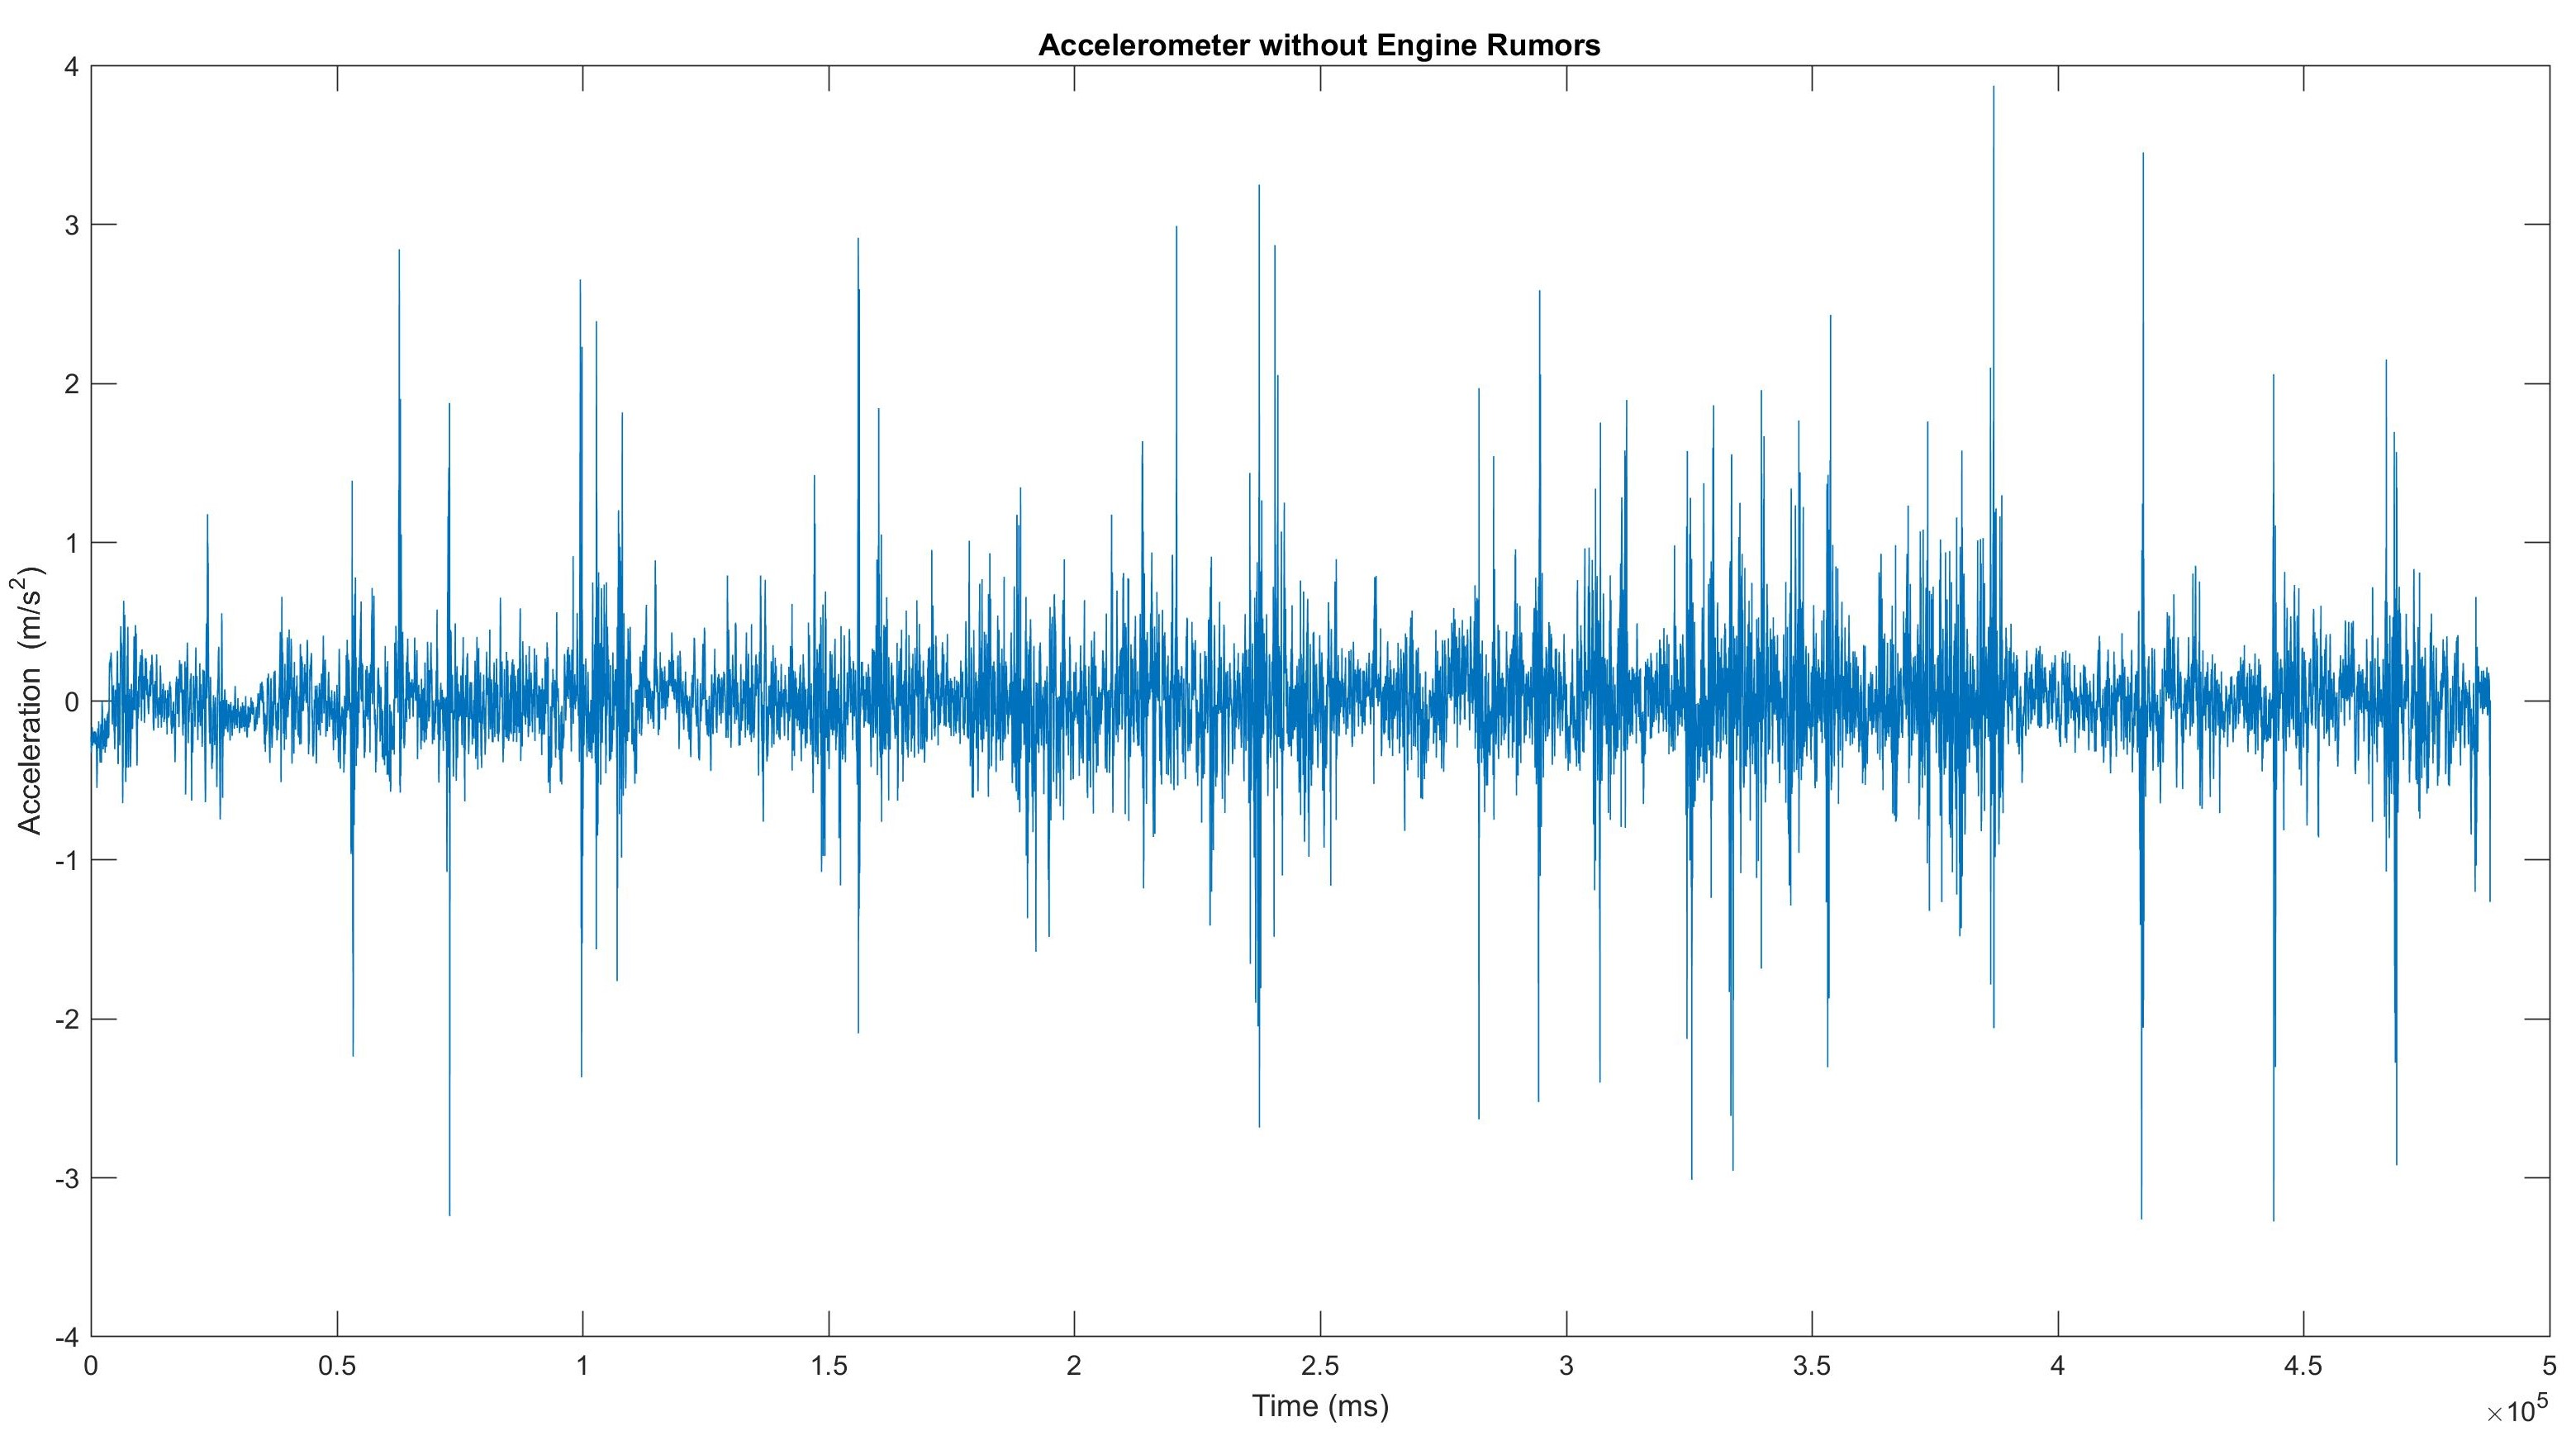
\includegraphics[scale=0.099]{NoRumors}} 
\subfloat[No Zero Velocity]{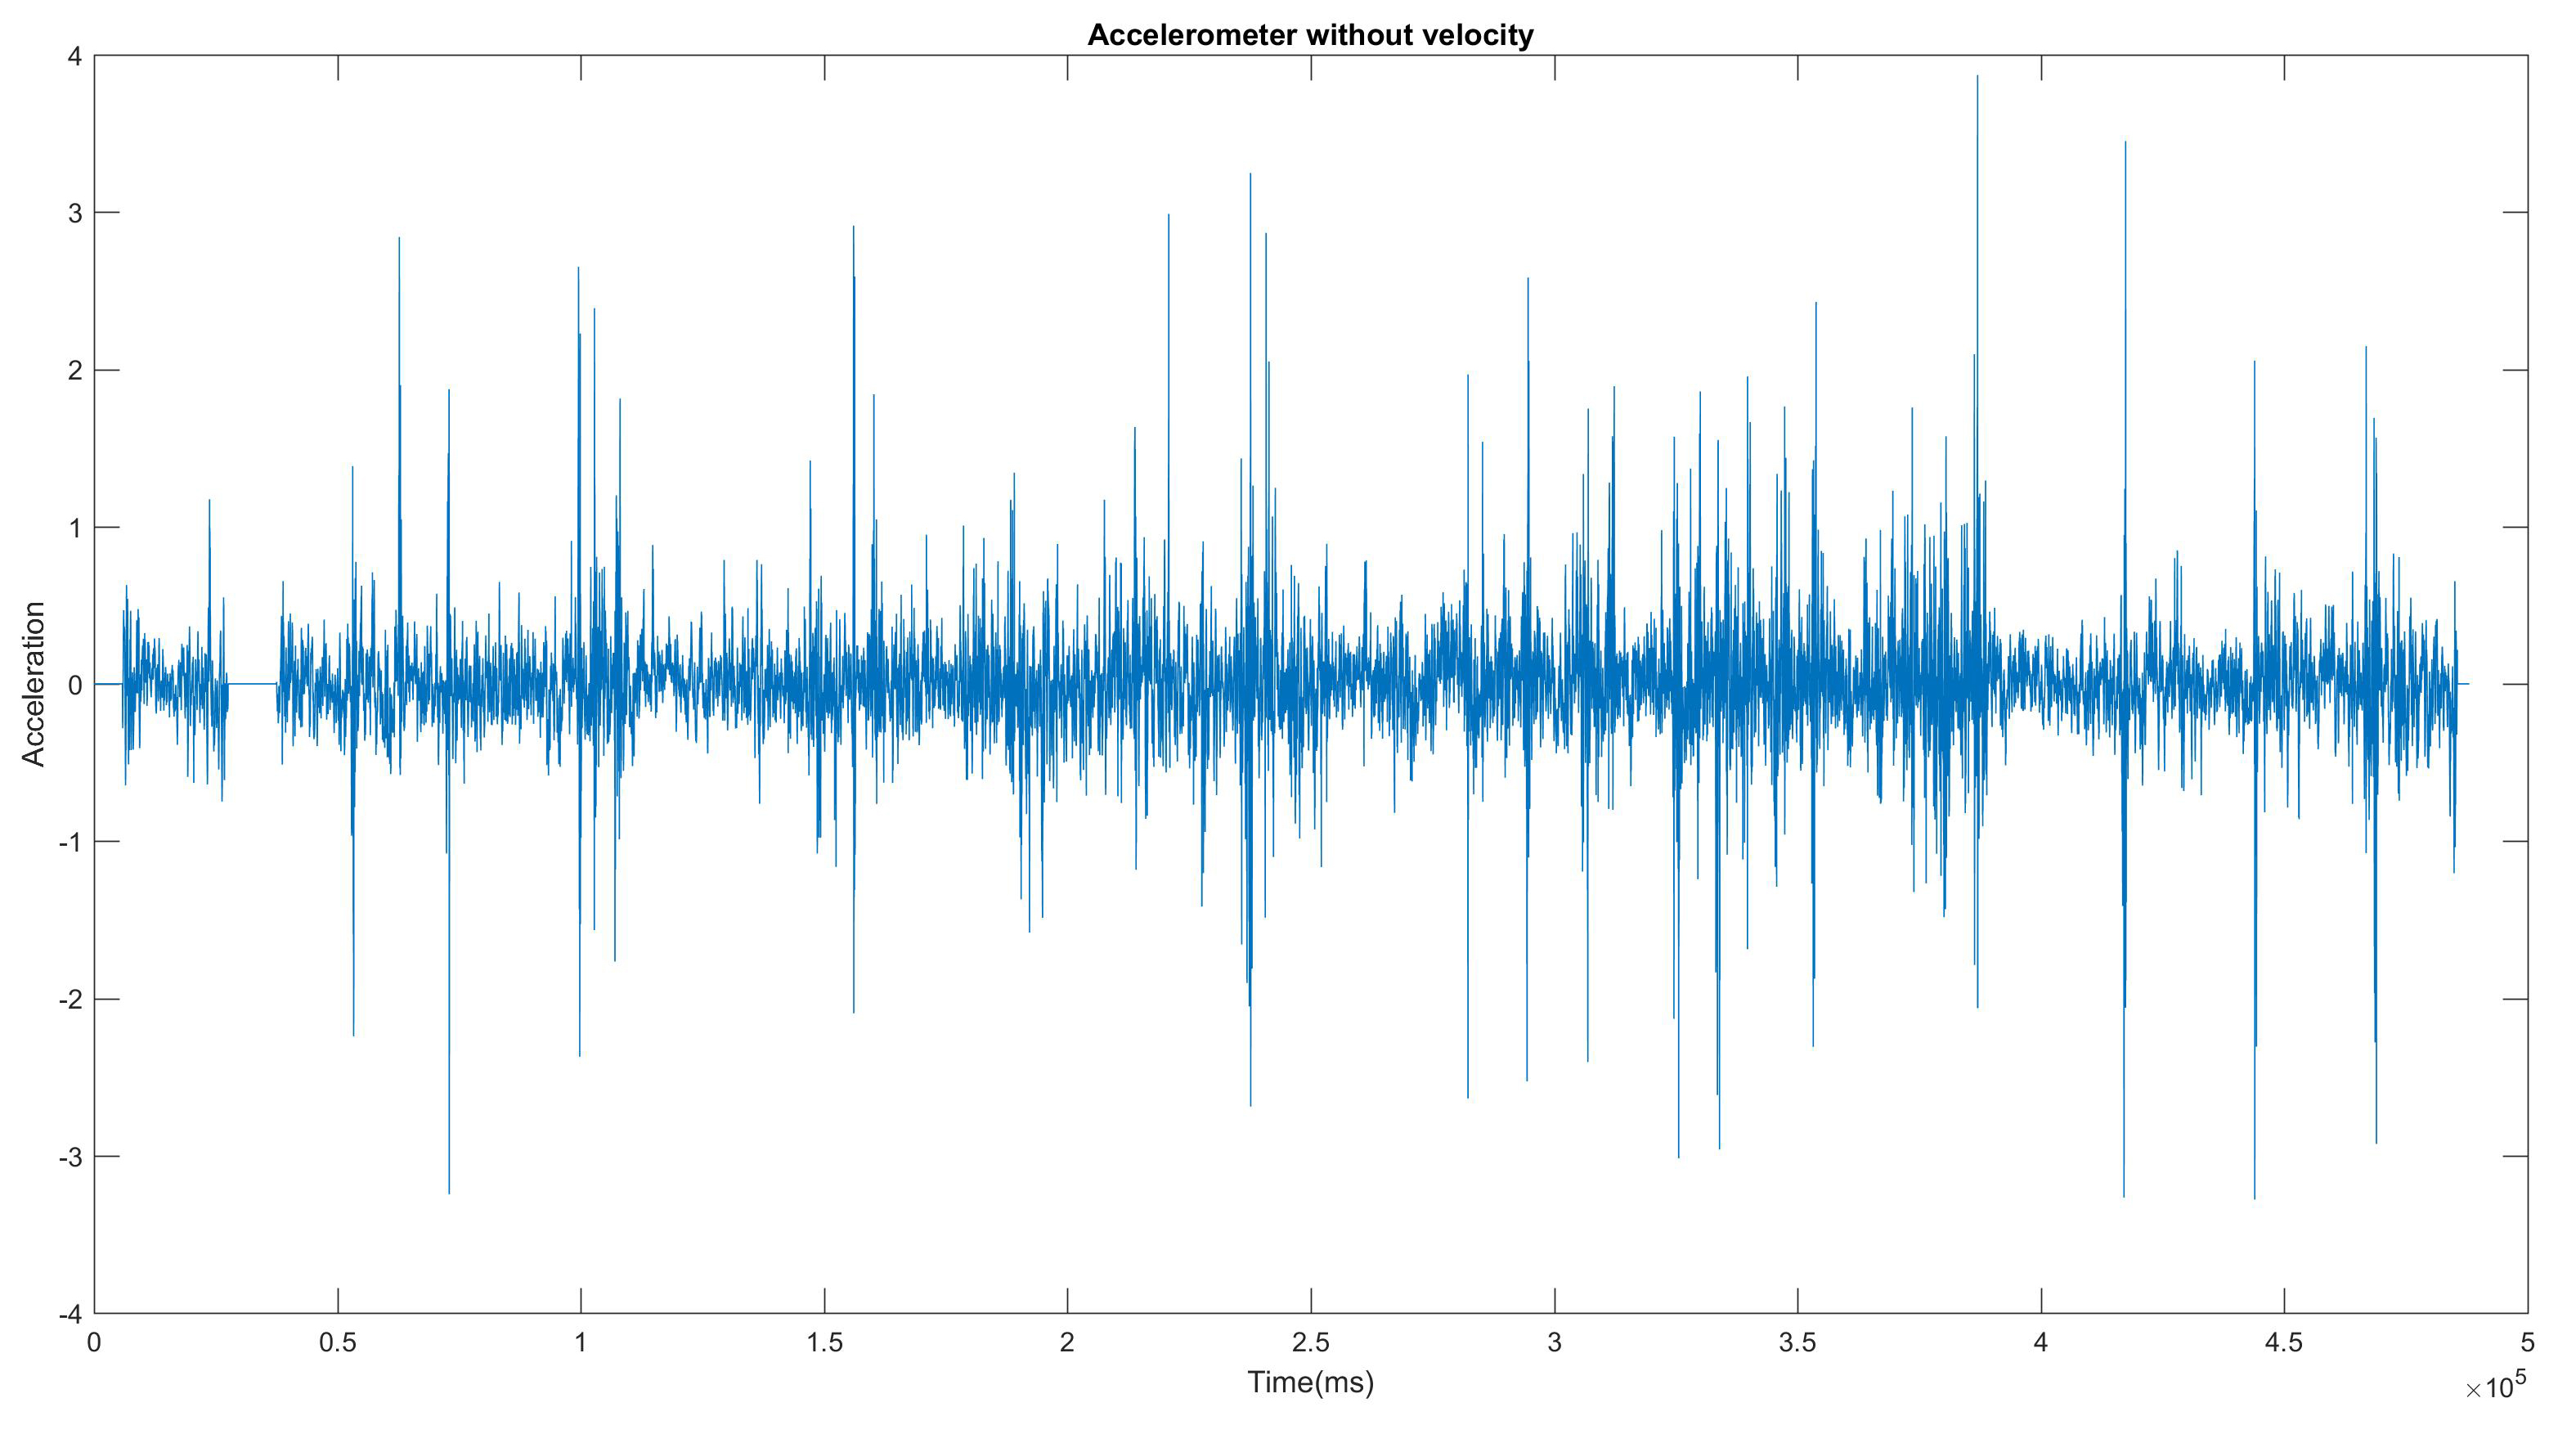
\includegraphics[scale=0.074]{NoVelocity}}

\centering
\subfloat[Overlapping]{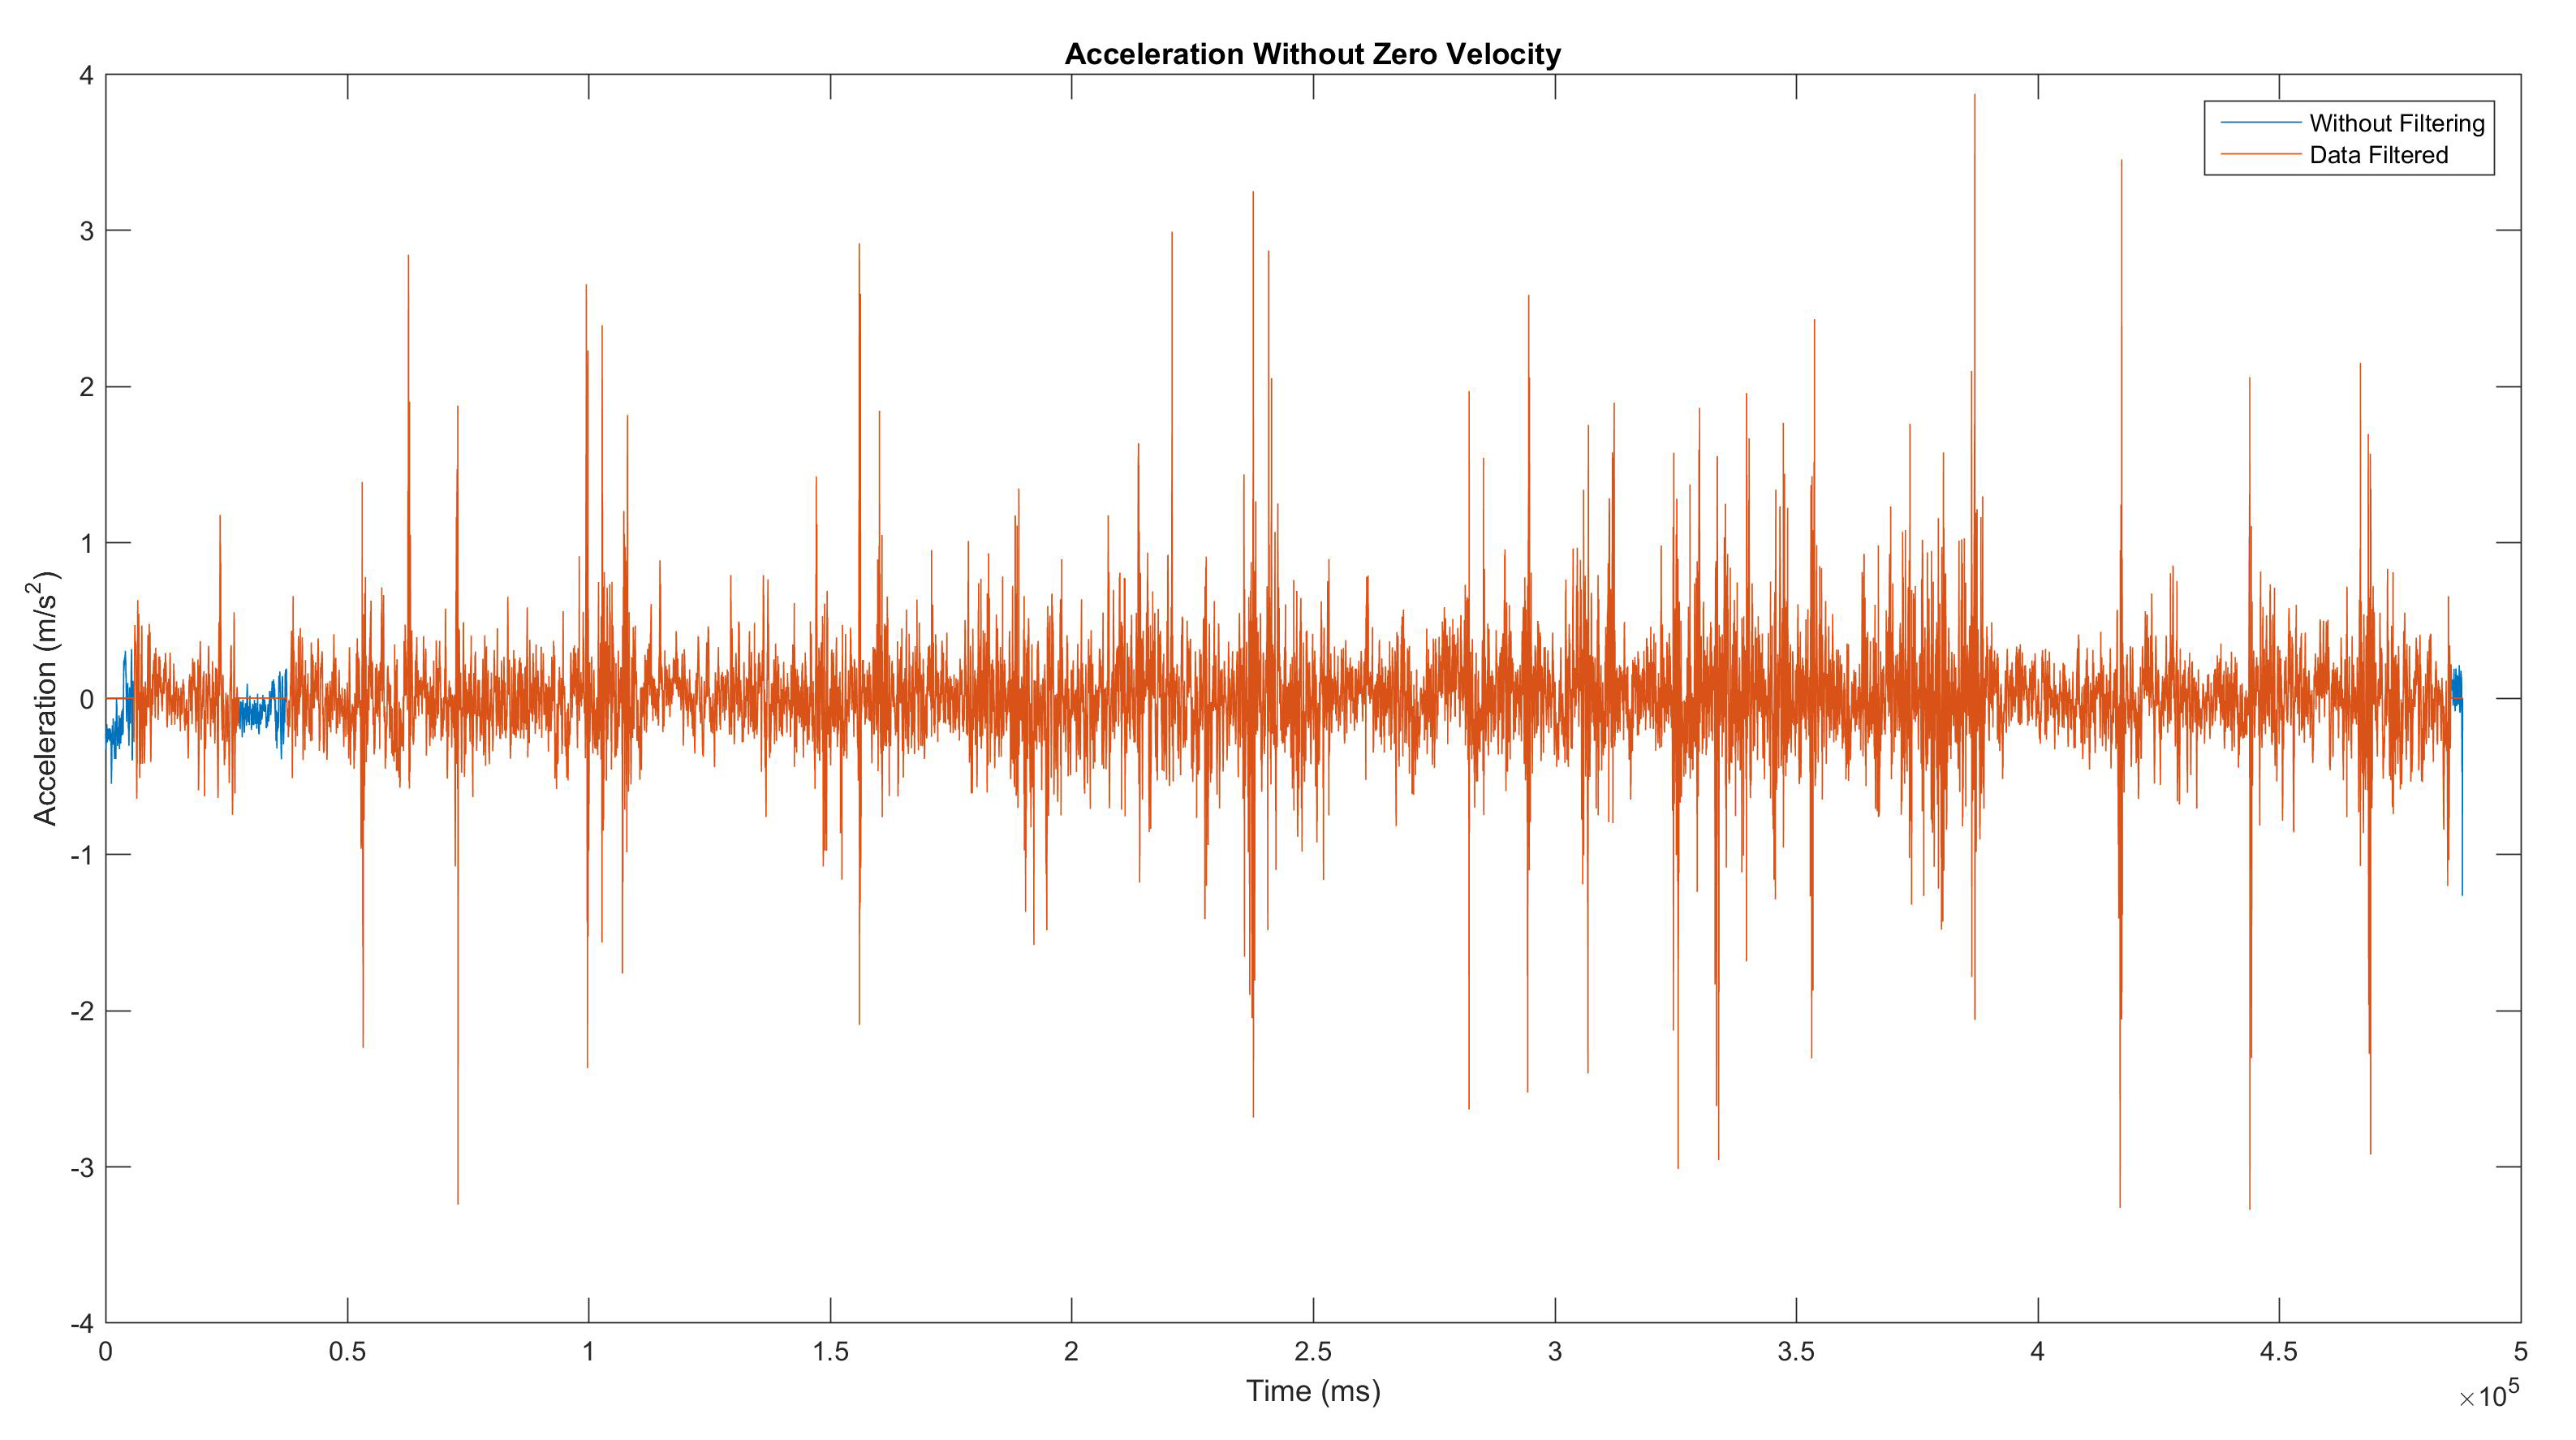
\includegraphics[scale=0.1]{NoVelocitySovrapposte}}

The original signal (a) is represent in blue, the filtered signal is represent in orange (b).

 \caption{Application of Zero Velocity Filter}
  \label{fig:Application of Zero Velocity Filter.}
\end{figure}


\subsection{Digital Filtering} \label{ssc:Digital Filtering}
For IRI calculation, vertical displacement is needed, so the accelerometer data must be subject to a double integration process. 
Unfortunately, accelerometers have an undesired phenomenon named drift associated with them produced by a small DC component\footnote{DC offset is a zero offset compensation. Refers to an electrical signal in which the value is shifted to a certain amount respect to the reference mass.} in the acceleration signal.
Ideally, there should be no DC from the accelerometer for the measurement of a vibration. The presence of drift can direct to high integration errors. If the acceleration signal was integrated without any proper filtering, the output could become unlimited over time. The figure \ref{fig:Integration of Raw Data} shows what usually occurs to an acceleration signal after a double integration. Figure \ref{fig:Integration of Raw Data}, is an example of acceleration signal that has a negative DC.
To resolve the drift problem, a filter can be used to remove the DC component from the acceleration signal. Through filtering before integration, drift errors can be eliminated.
For the initial conditions as discusses in \ref{ch:Data Analysis}, a solution is to use filtering.  
After the acceleration signal is integrated, it will possibly have a DC component. Again a filter can be used to remove that DC component of the signal. Furthermore, after the velocity signal is integrated to get the position, the position signal can be filtered as well.
Filtering is a particular frequency process that attenuates certain bands of frequencies while passing others. These filters will pass the high-frequency content of a signal while rejecting the low. The specifications of a filter are its cutoff frequency, passband attenuation, and stop-band attenuation. 
\begin{center}\textit{It is convenient if the filters are identical to each other to simplify the design.}\end{center}


There are two types of filters in the digital area: Infinite Impulse Response (IIR) filters and Finite Impulse Response (FIR) filters. 

\subsubsection{Finite Impulse Response} \label{ssc:Finite Impulse Response}
Finite Impulse Response, (FIR), is a type of digital filter characterised by a finite response, that, it is cancelled at a finite time.
A FIR filter is described by the following difference equation:

\begin{center}
{\large $y[n] = b_{o} \thinspace x[n] \thinspace  + b_{1} \thinspace  x[n-1] + ... + b_{N} \thinspace  x[n - N] = \thinspace  \sum\limits_{i=0}^{N} \thinspace  b_{i} \thinspace  x[n-i]$}

\end{center}

\noindent Where: 
$x[n]$ is the input signal, $y[n]$ is the output signal, $N$ is the filter order, and $b_{i}$ is the value of the impulse response at instant $i$.
This filter is useful for the double integration process. It is recommended to use it because its phase response is linear, which is desired because different frequencies passing through the filter will have the same time delay.
A disadvantage is that the order can be very high, and lead to excessive computations.
For application to a vehicle road test, there is an interest in processing low-frequency signals. So the filter must have a low cutoff frequency with a clear transition band, making the order of the filter high.

\paragraph{Moving Average}\label{p:moving_average} \leavevmode\\\\
An example of FIR filter is the moving average, commonly used in road pavement profiles, that defines the point $A_{i}$ as the average of the points close to that one, for a base window of length $n$ \cite{little_book}, defined like follow:
\begin{center}
{\large $ A_{i} = \dfrac{1}{n} \thinspace  \sum\limits_{k=i}^{k=i+n} \thinspace  A_{k}$}
\end{center}

\noindent An example of application of the moving average filter is shown in the figure below:
 
\begin{figure}[H]	
\subfloat[Unfiltered Signal]{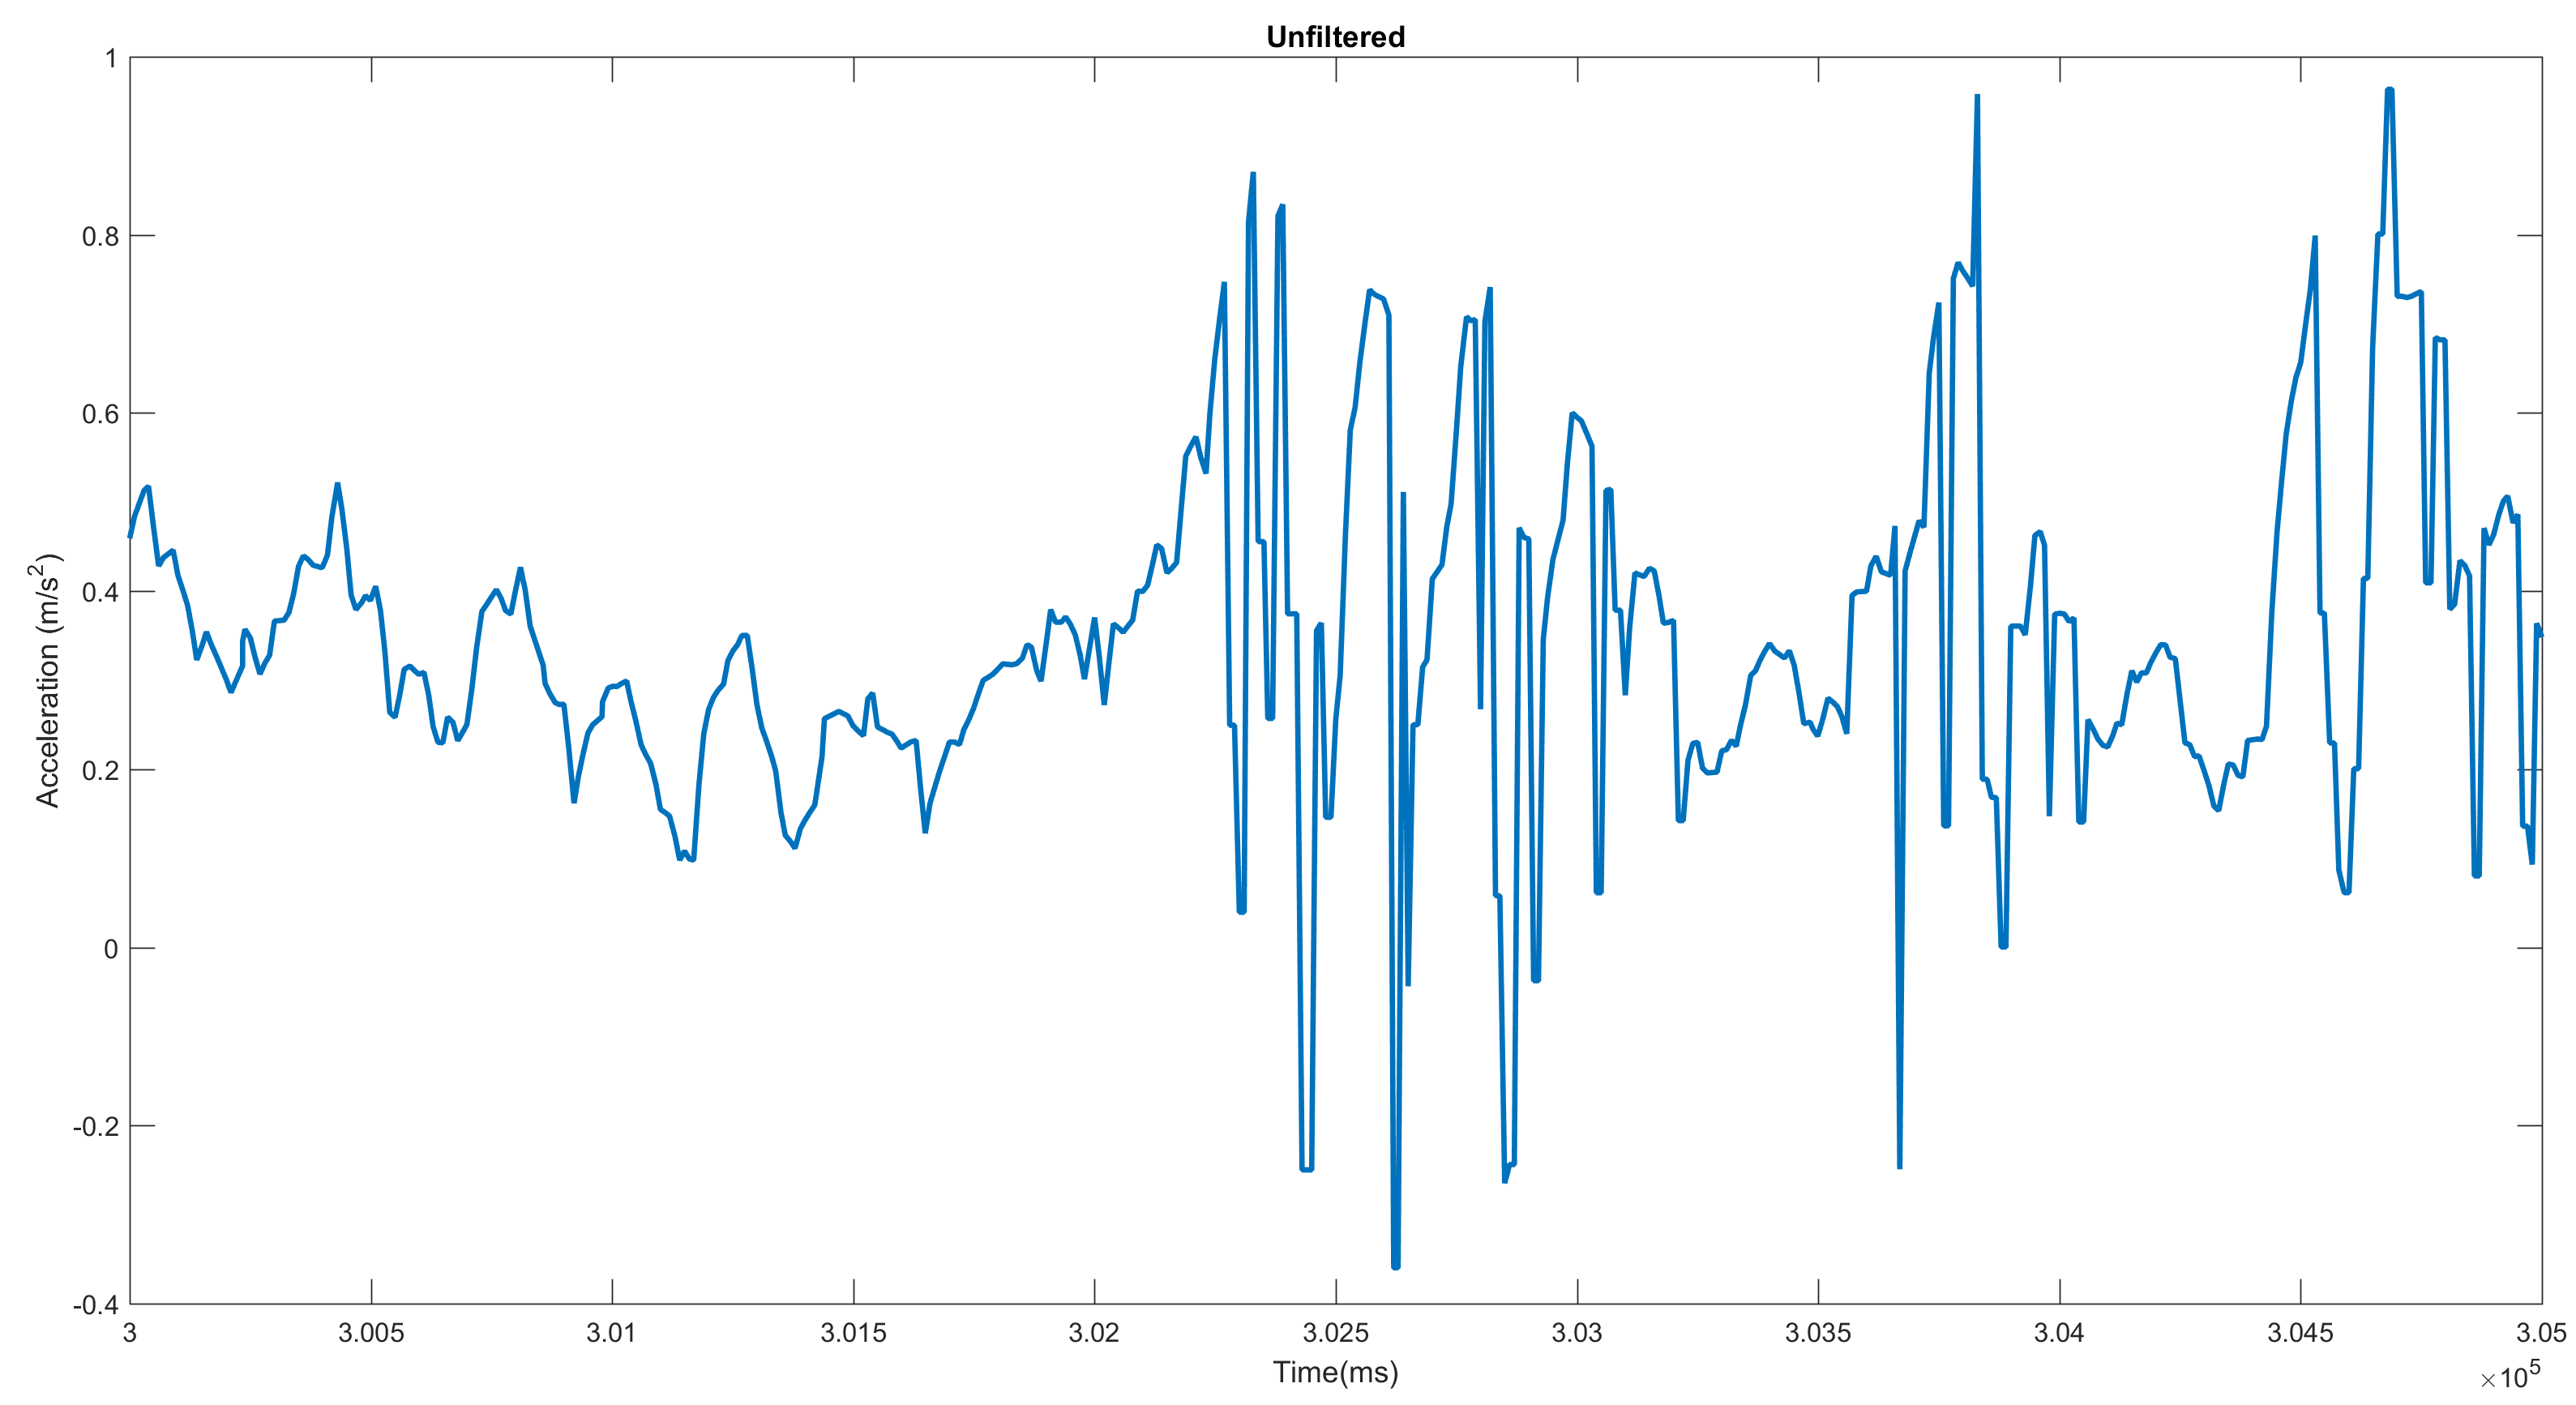
\includegraphics[scale=0.1]{NoMovingFiltered}}    
\subfloat[Filtered Signal]{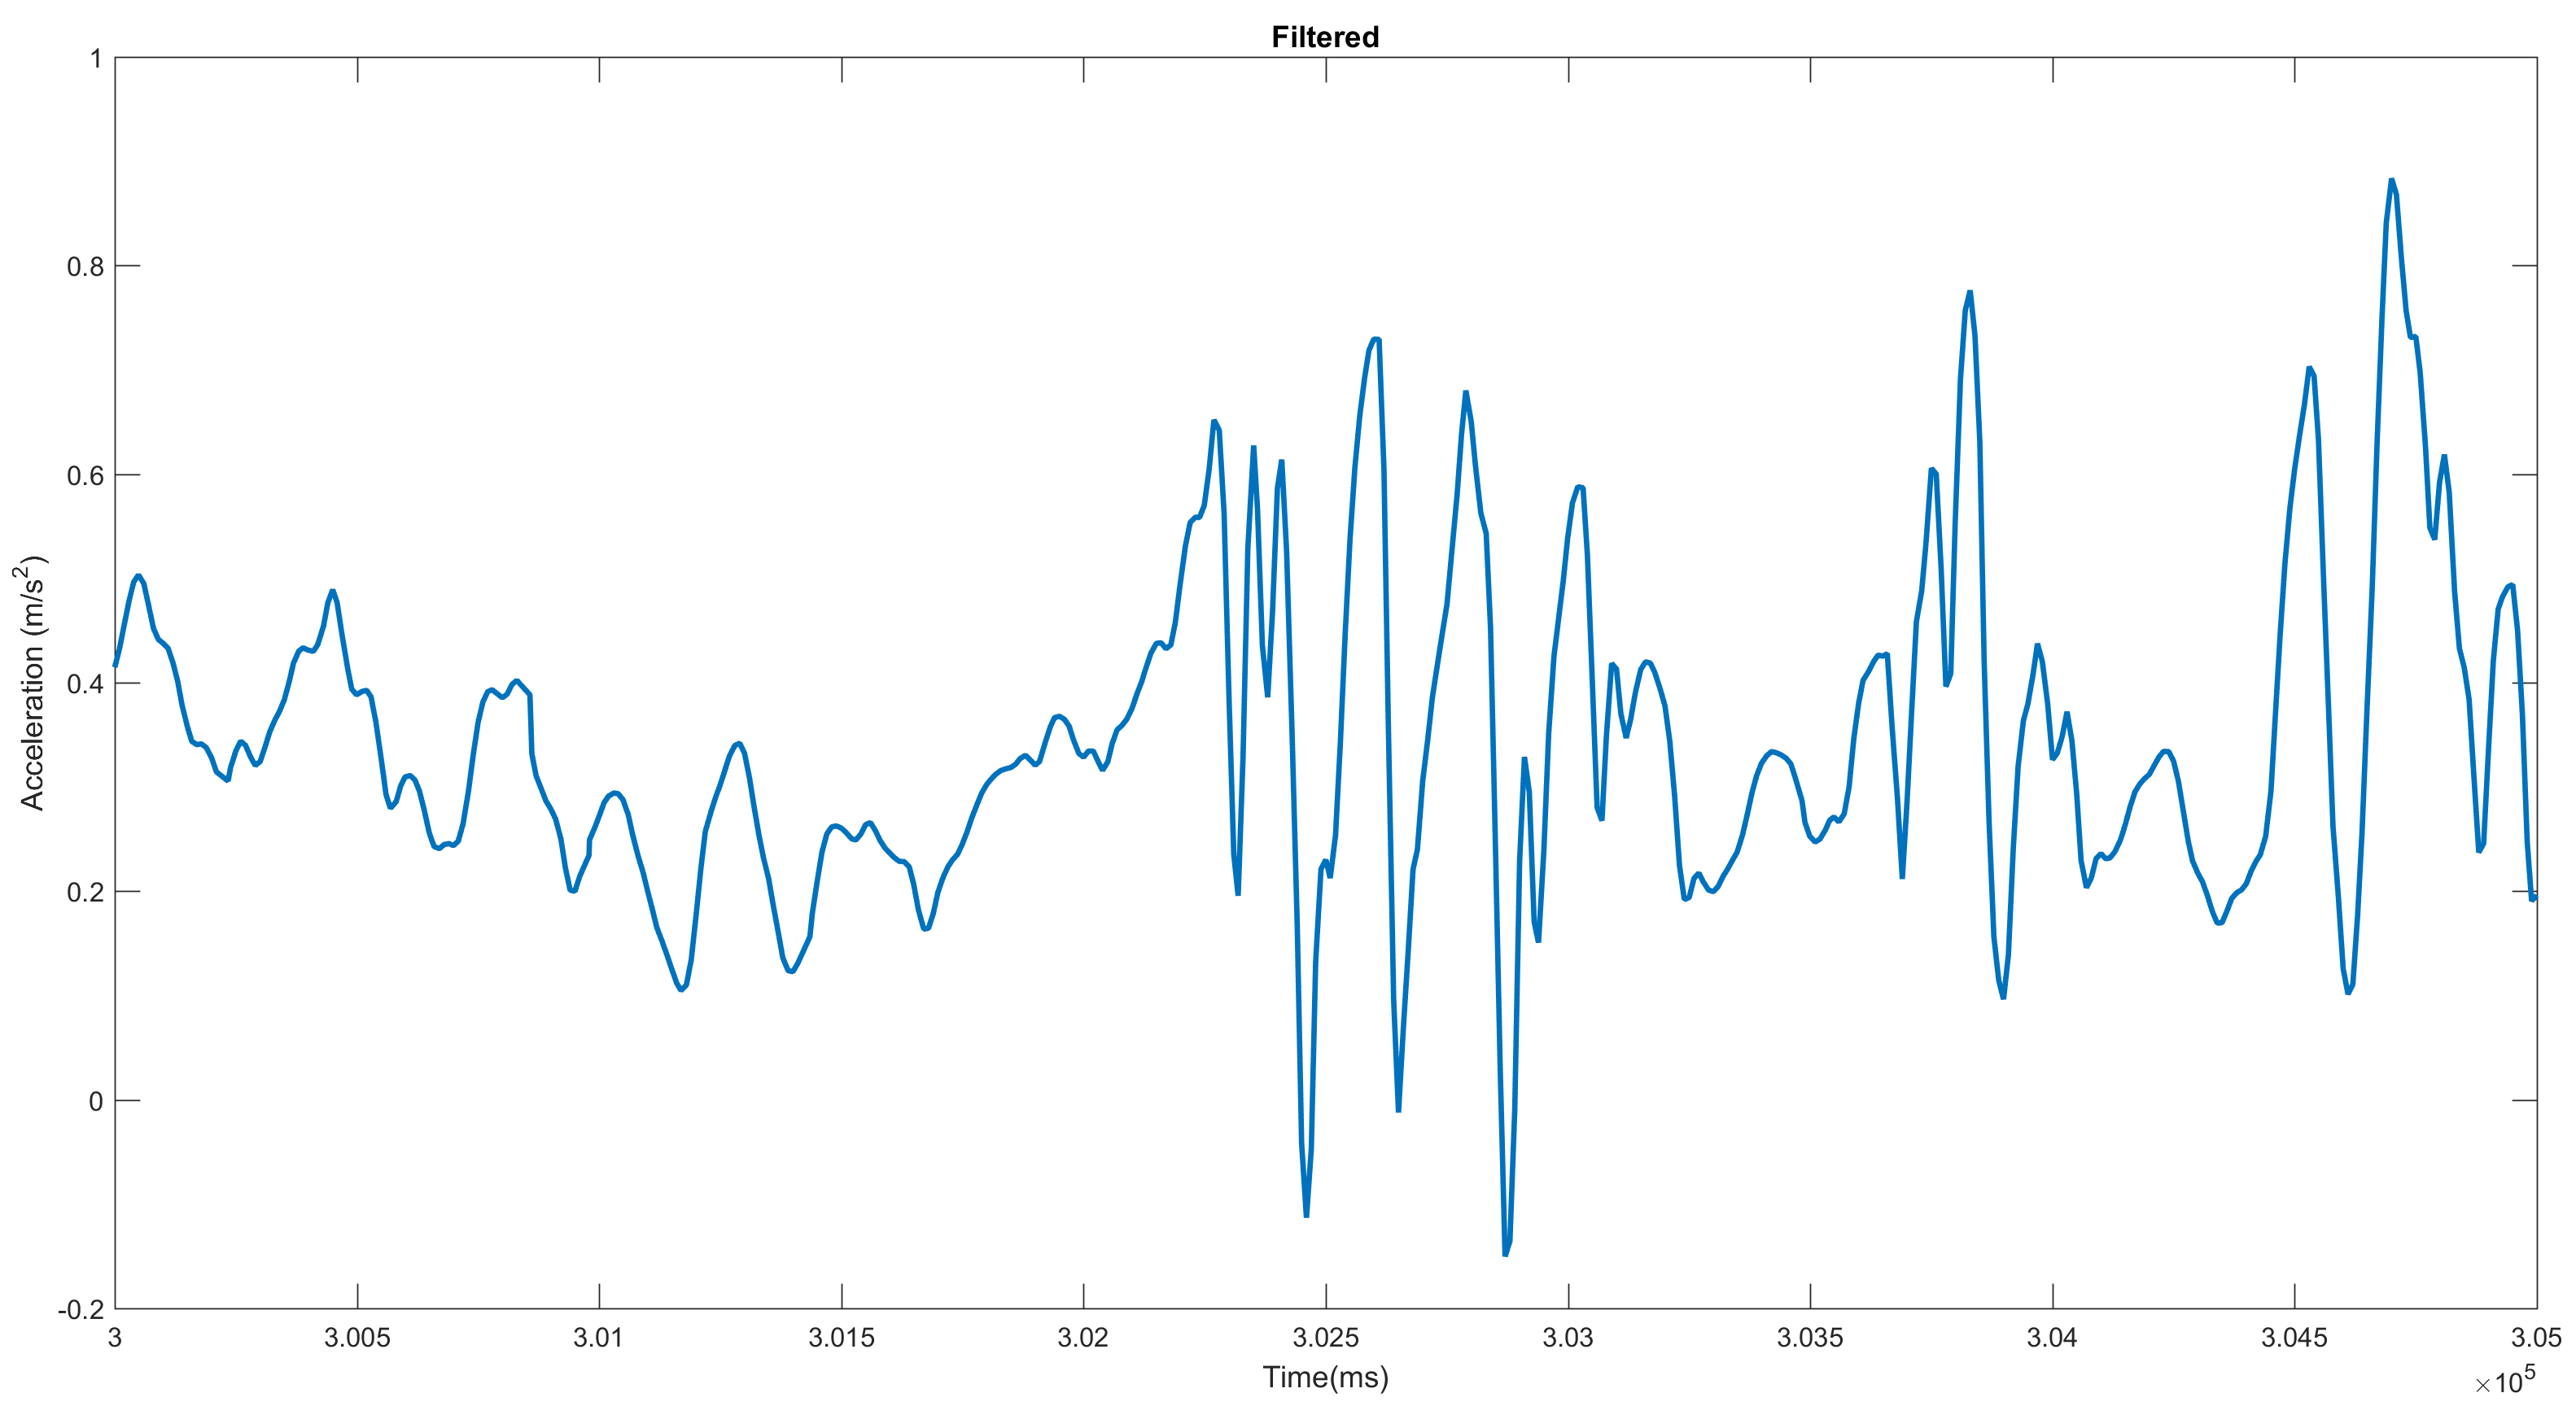
\includegraphics[scale=0.1]{MovingFiltered}}

\centering
\subfloat[Signal Overlapping]{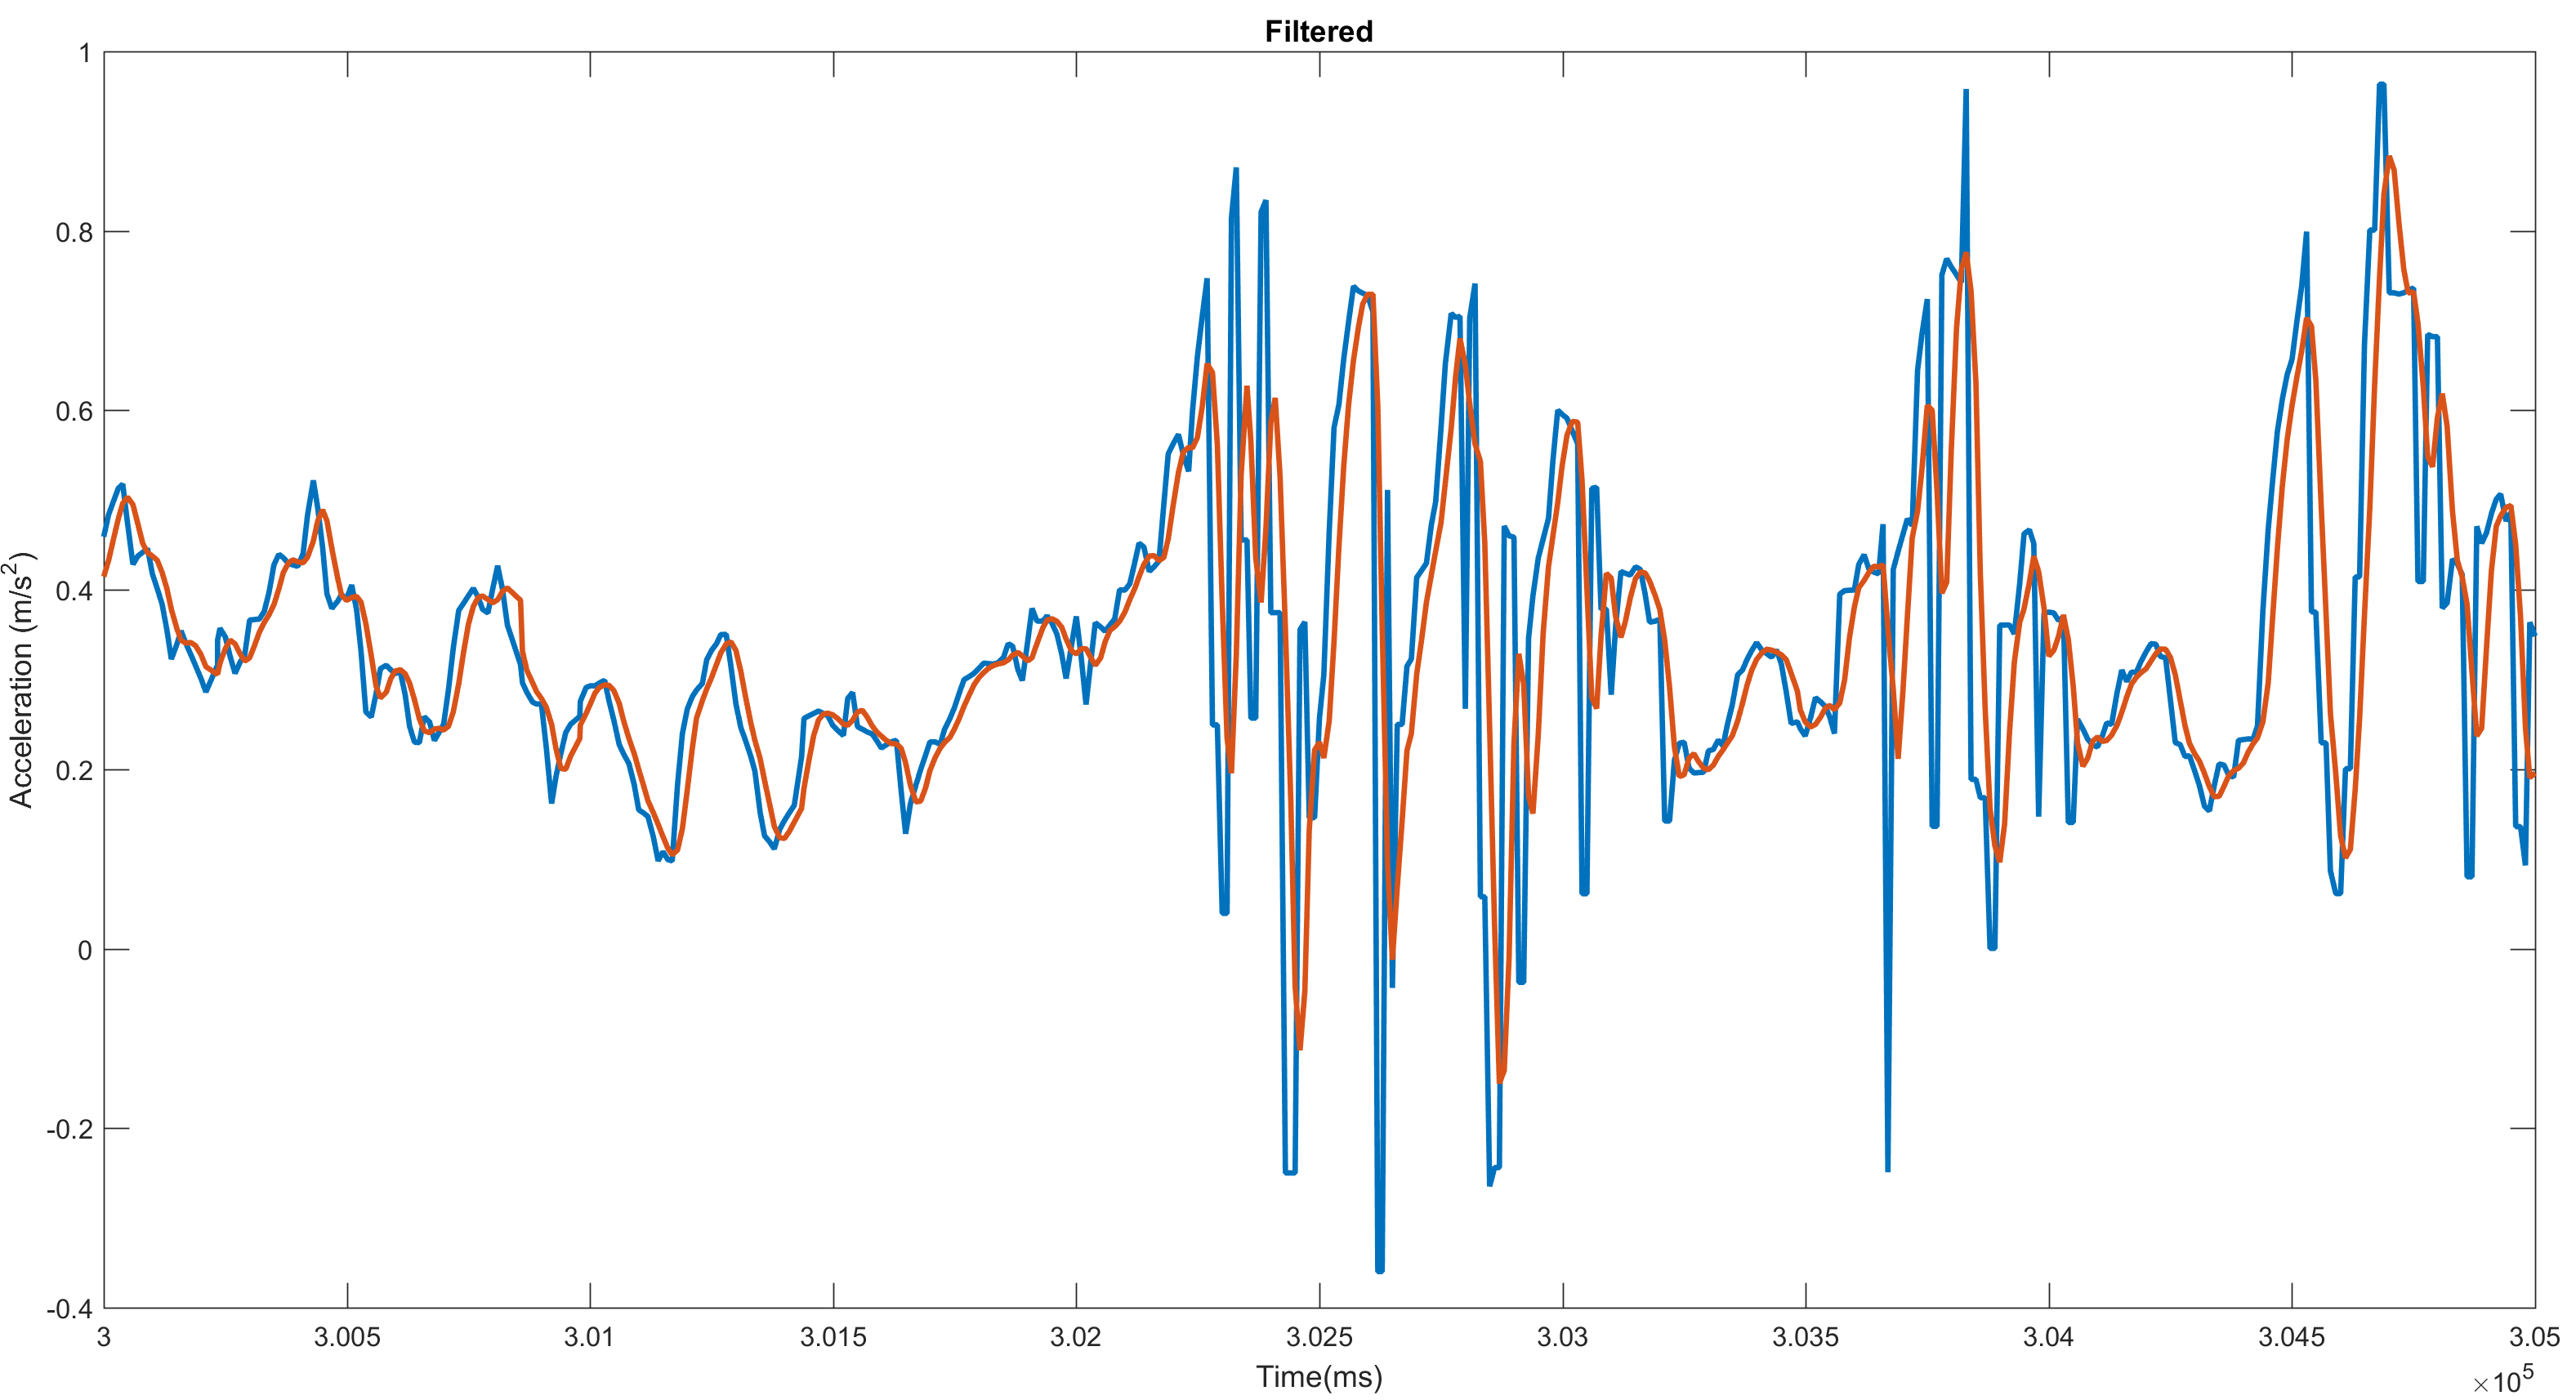
\includegraphics[scale=0.15]{TotalFiltered}}

The original signal (a) is represent in blue, the filtered signal is represent in orange (b).
 \caption{Application of Moving Average Filter}
  \label{fig:Application of Moving Average	 Filter.}
\end{figure}
\clearpage
\subsubsection{Infinite Impulse Response} \label{ssc:Infite Impulse Response}
In signals theory, Infinite Impulse Response (IIR) is a dynamic system whose impulsive response is not anything for an infinite amount of time.
IIR filtering is an alternative approach, that uses a recursive difference equation to represent the filter.
\begin{center}
\begin{large}
$ y[n] = a_{0} \thinspace (\sum\limits_{i=0}^{P}\thinspace  b_{i} \thinspace x[n-1] + \sum\limits_{j=1}^{Q} \thinspace  a_{j} \thinspace  y[n-j])$

\end{large}\end{center}



\noindent Where $y[n]$ is the output and $x[n]$ is the input, the output is written as a combination of present and past inputs and past outputs.

\noindent IIR has an advantage respect FIR filters, regard to the filter order. An IIR filter has a very lower order than FIR, so the computations can be done faster. However, its phase response is not linear like the FIR’s response. The physical meaning of this is if a signal is passed through this filter, different frequency components of this signal will be delayed by different lengths of time, causing distortion.
There is a way to overcome the problem of having a non-linear phase with the IIR filter. 
Filter the signal, time reverses the signal, and filter it again with the same filter. A MATLAB command \textit{(filtfilt) } allow us to perform this operation. 

\subsubsection{Low Pass Filter} \label{ssc:Low Pass Filter}
A Low-Pass Filter is a filter that allows the passage of signals below a cutoff frequency (known as the passband) and attenuates signals above the cutoff frequency (known as the stopband). The exact frequency response of the filter depends on the filter design.
A low-pass filter is the complement of a high-pass filter.
Through removing some frequencies, the filter creates a smoothing effect. The filter produces slow changes in output values to make it easier to see trends and increase the signal-to-noise ratio with minimal signal degradation.
Low-pass filters provide a smoother form of a signal, removing the short-term fluctuations, and leaving the longer-term trend.
Low-pass filters, especially moving average filters or Savitzky-Golay filters, are often used to smooth signals, remove noise, perform data averaging.
Other common design methods for low-pass FIR-based filters include Kaiser window and equiripple.  
Design methods for IIR-based filters include Butterworth, Chebyshev (Type-I and Type-II), and elliptic.

\noindent Below is shown an example of application of Low-Pass-FIR filter on a Signal, with a Sample Rate of $1000$ $Hz$ and a Cutoff Frequency of $150$ $Hz$.

 
\begin{figure}[H]	
\centering 

\subfloat[Filter Response]{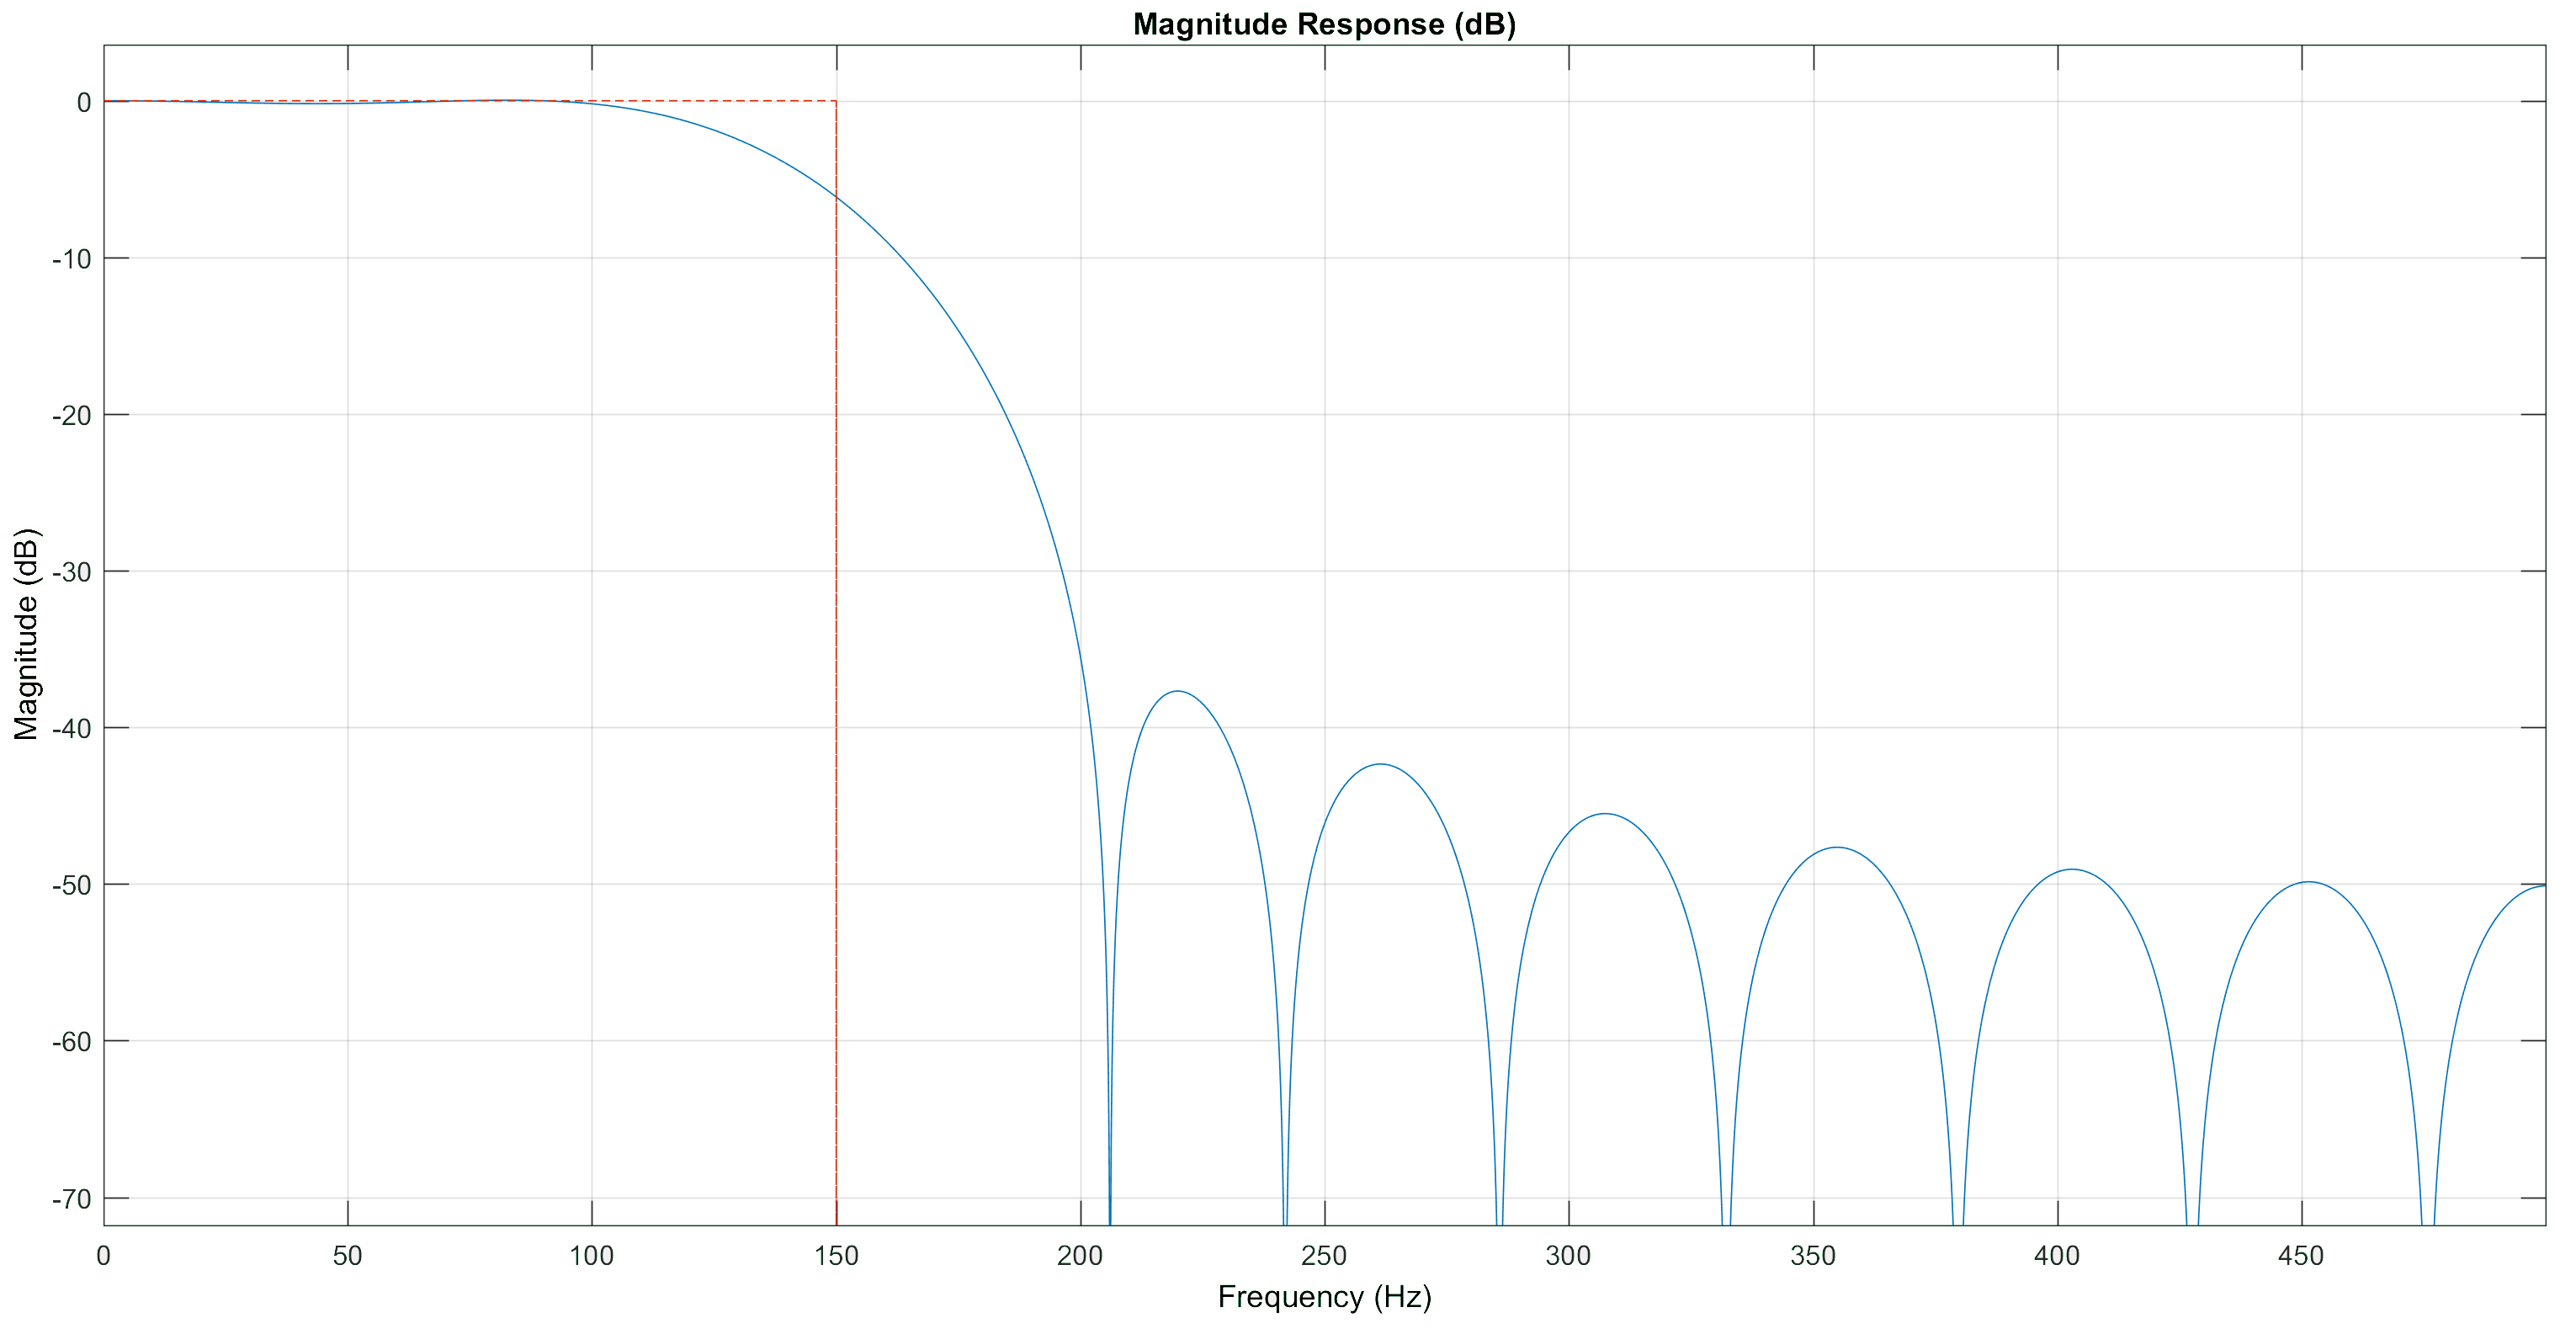
\includegraphics[scale=0.40]{LWPResponse}}    

\subfloat[Unfiltered]{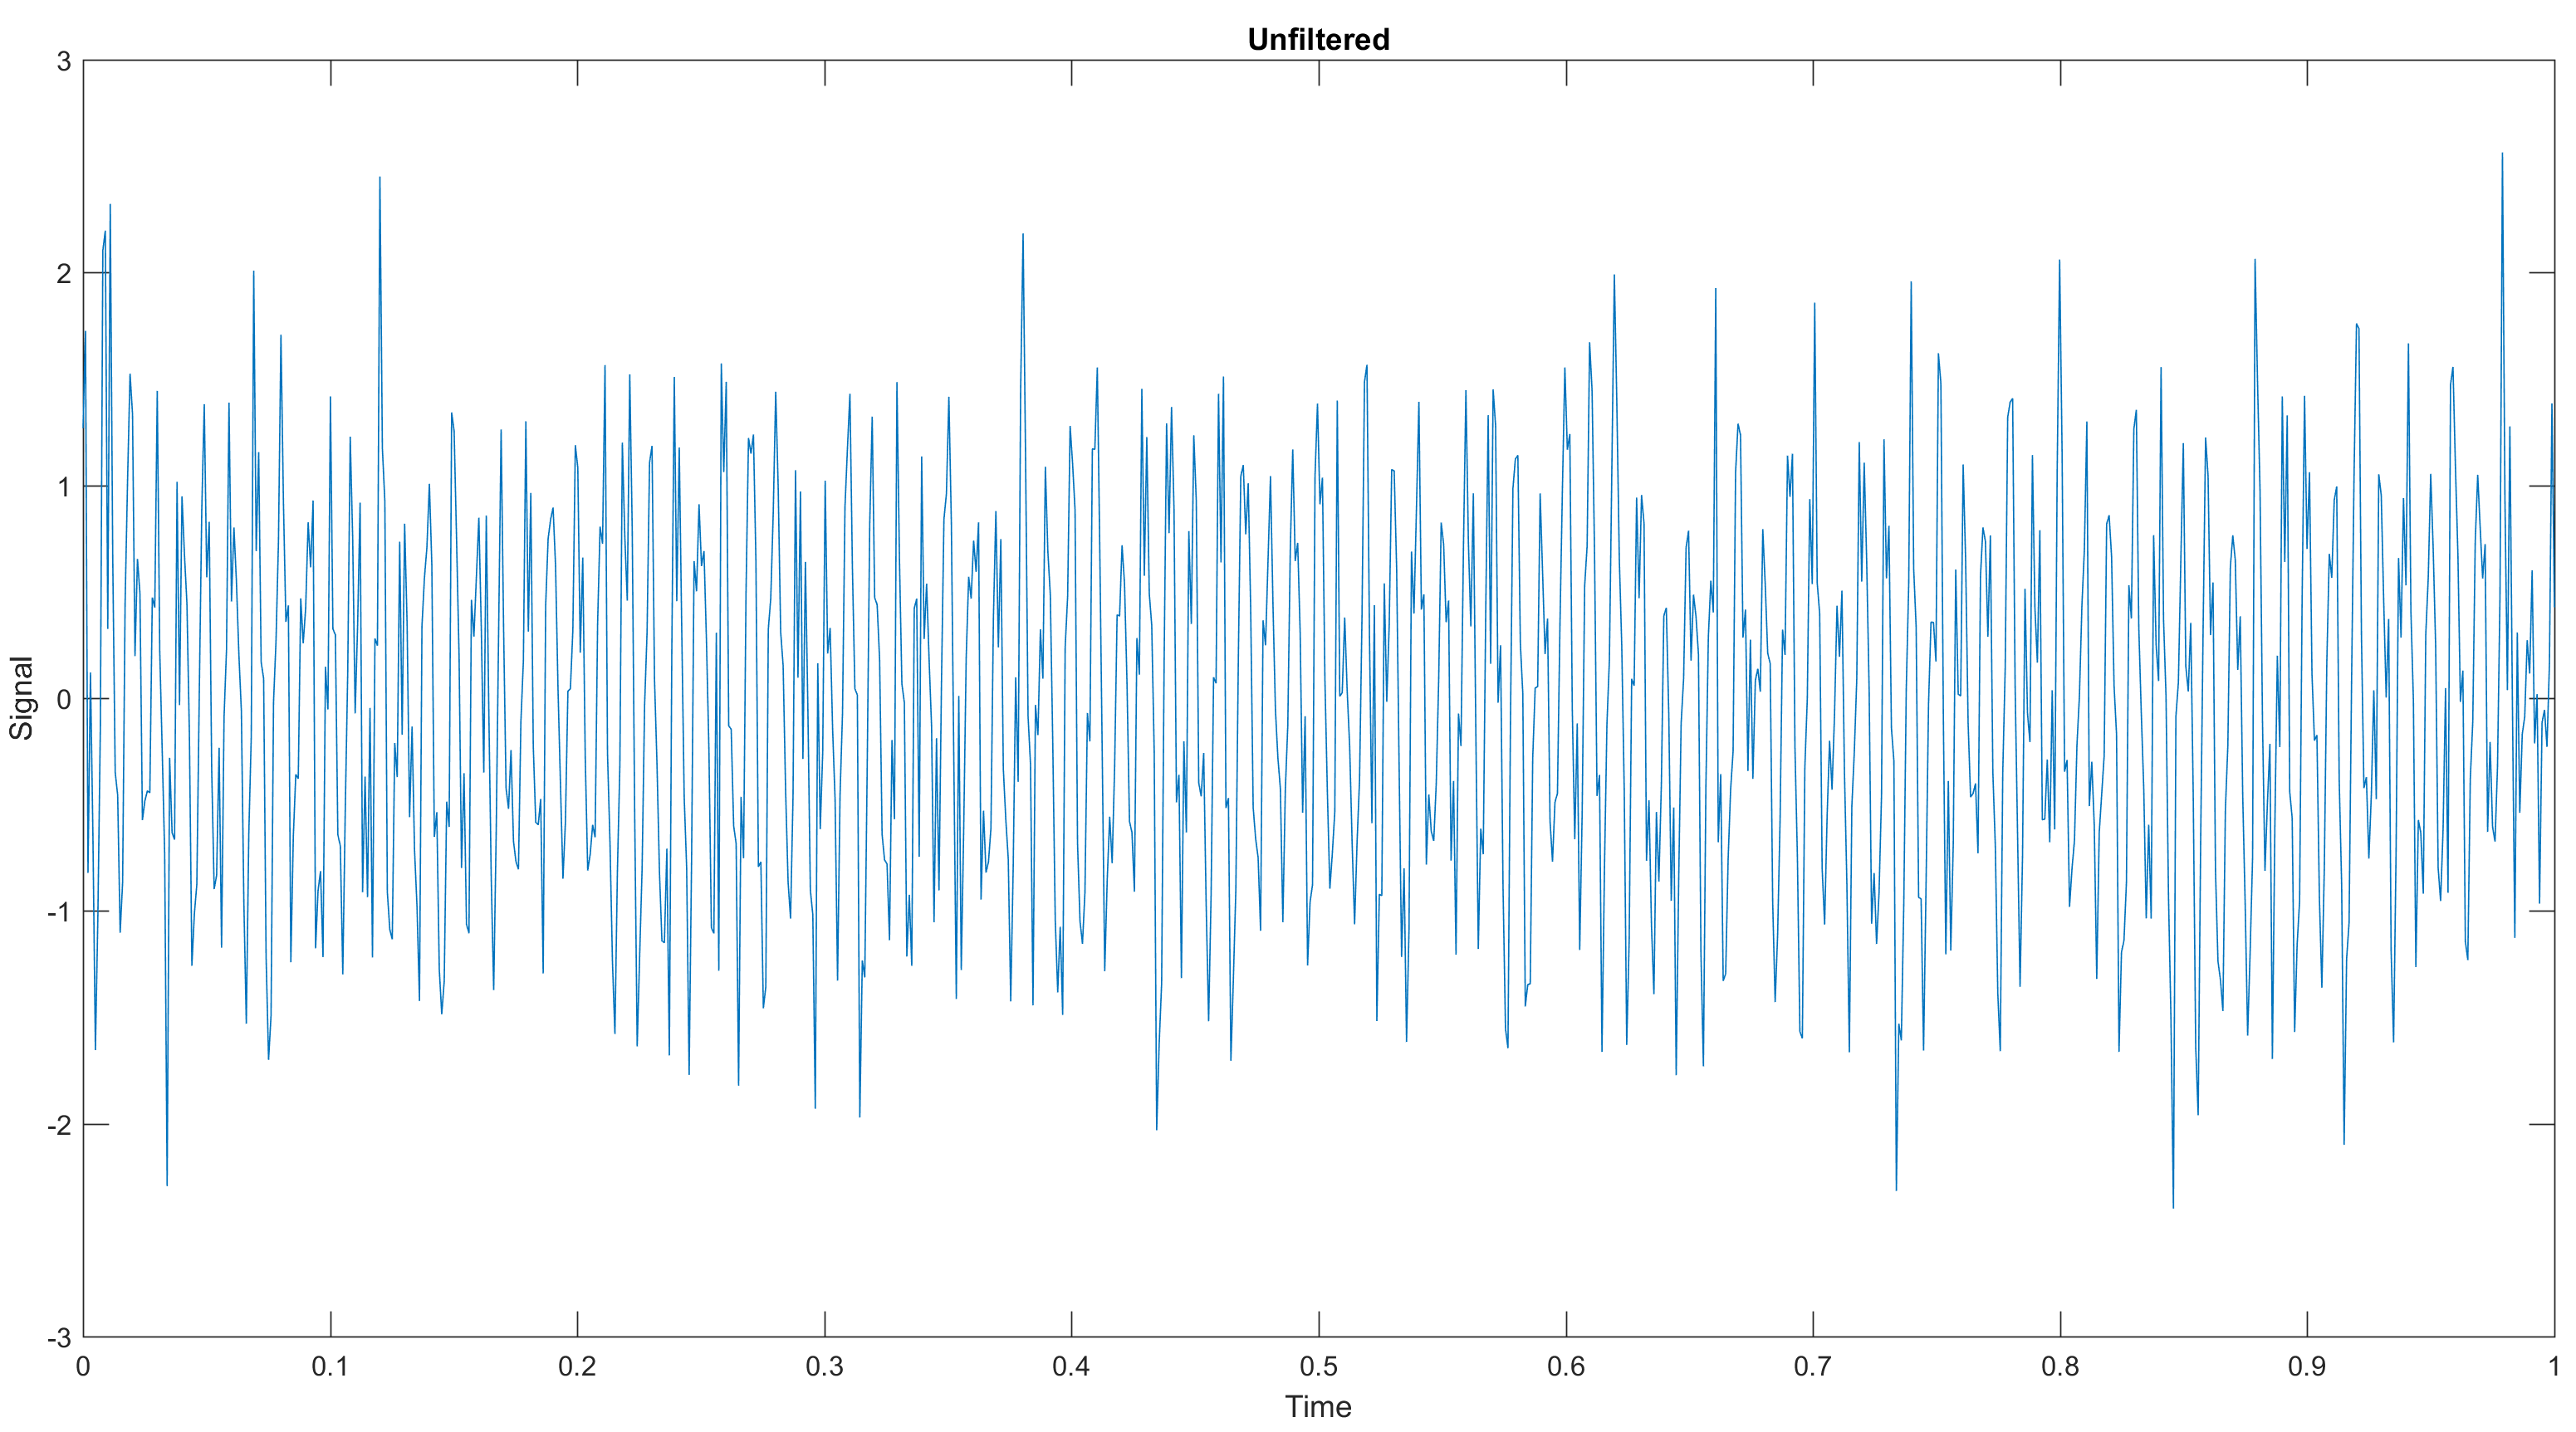
\includegraphics[scale=0.16]{LWPUnfitltered}}\label{fig:NoFilter}


\subfloat[Filtered]{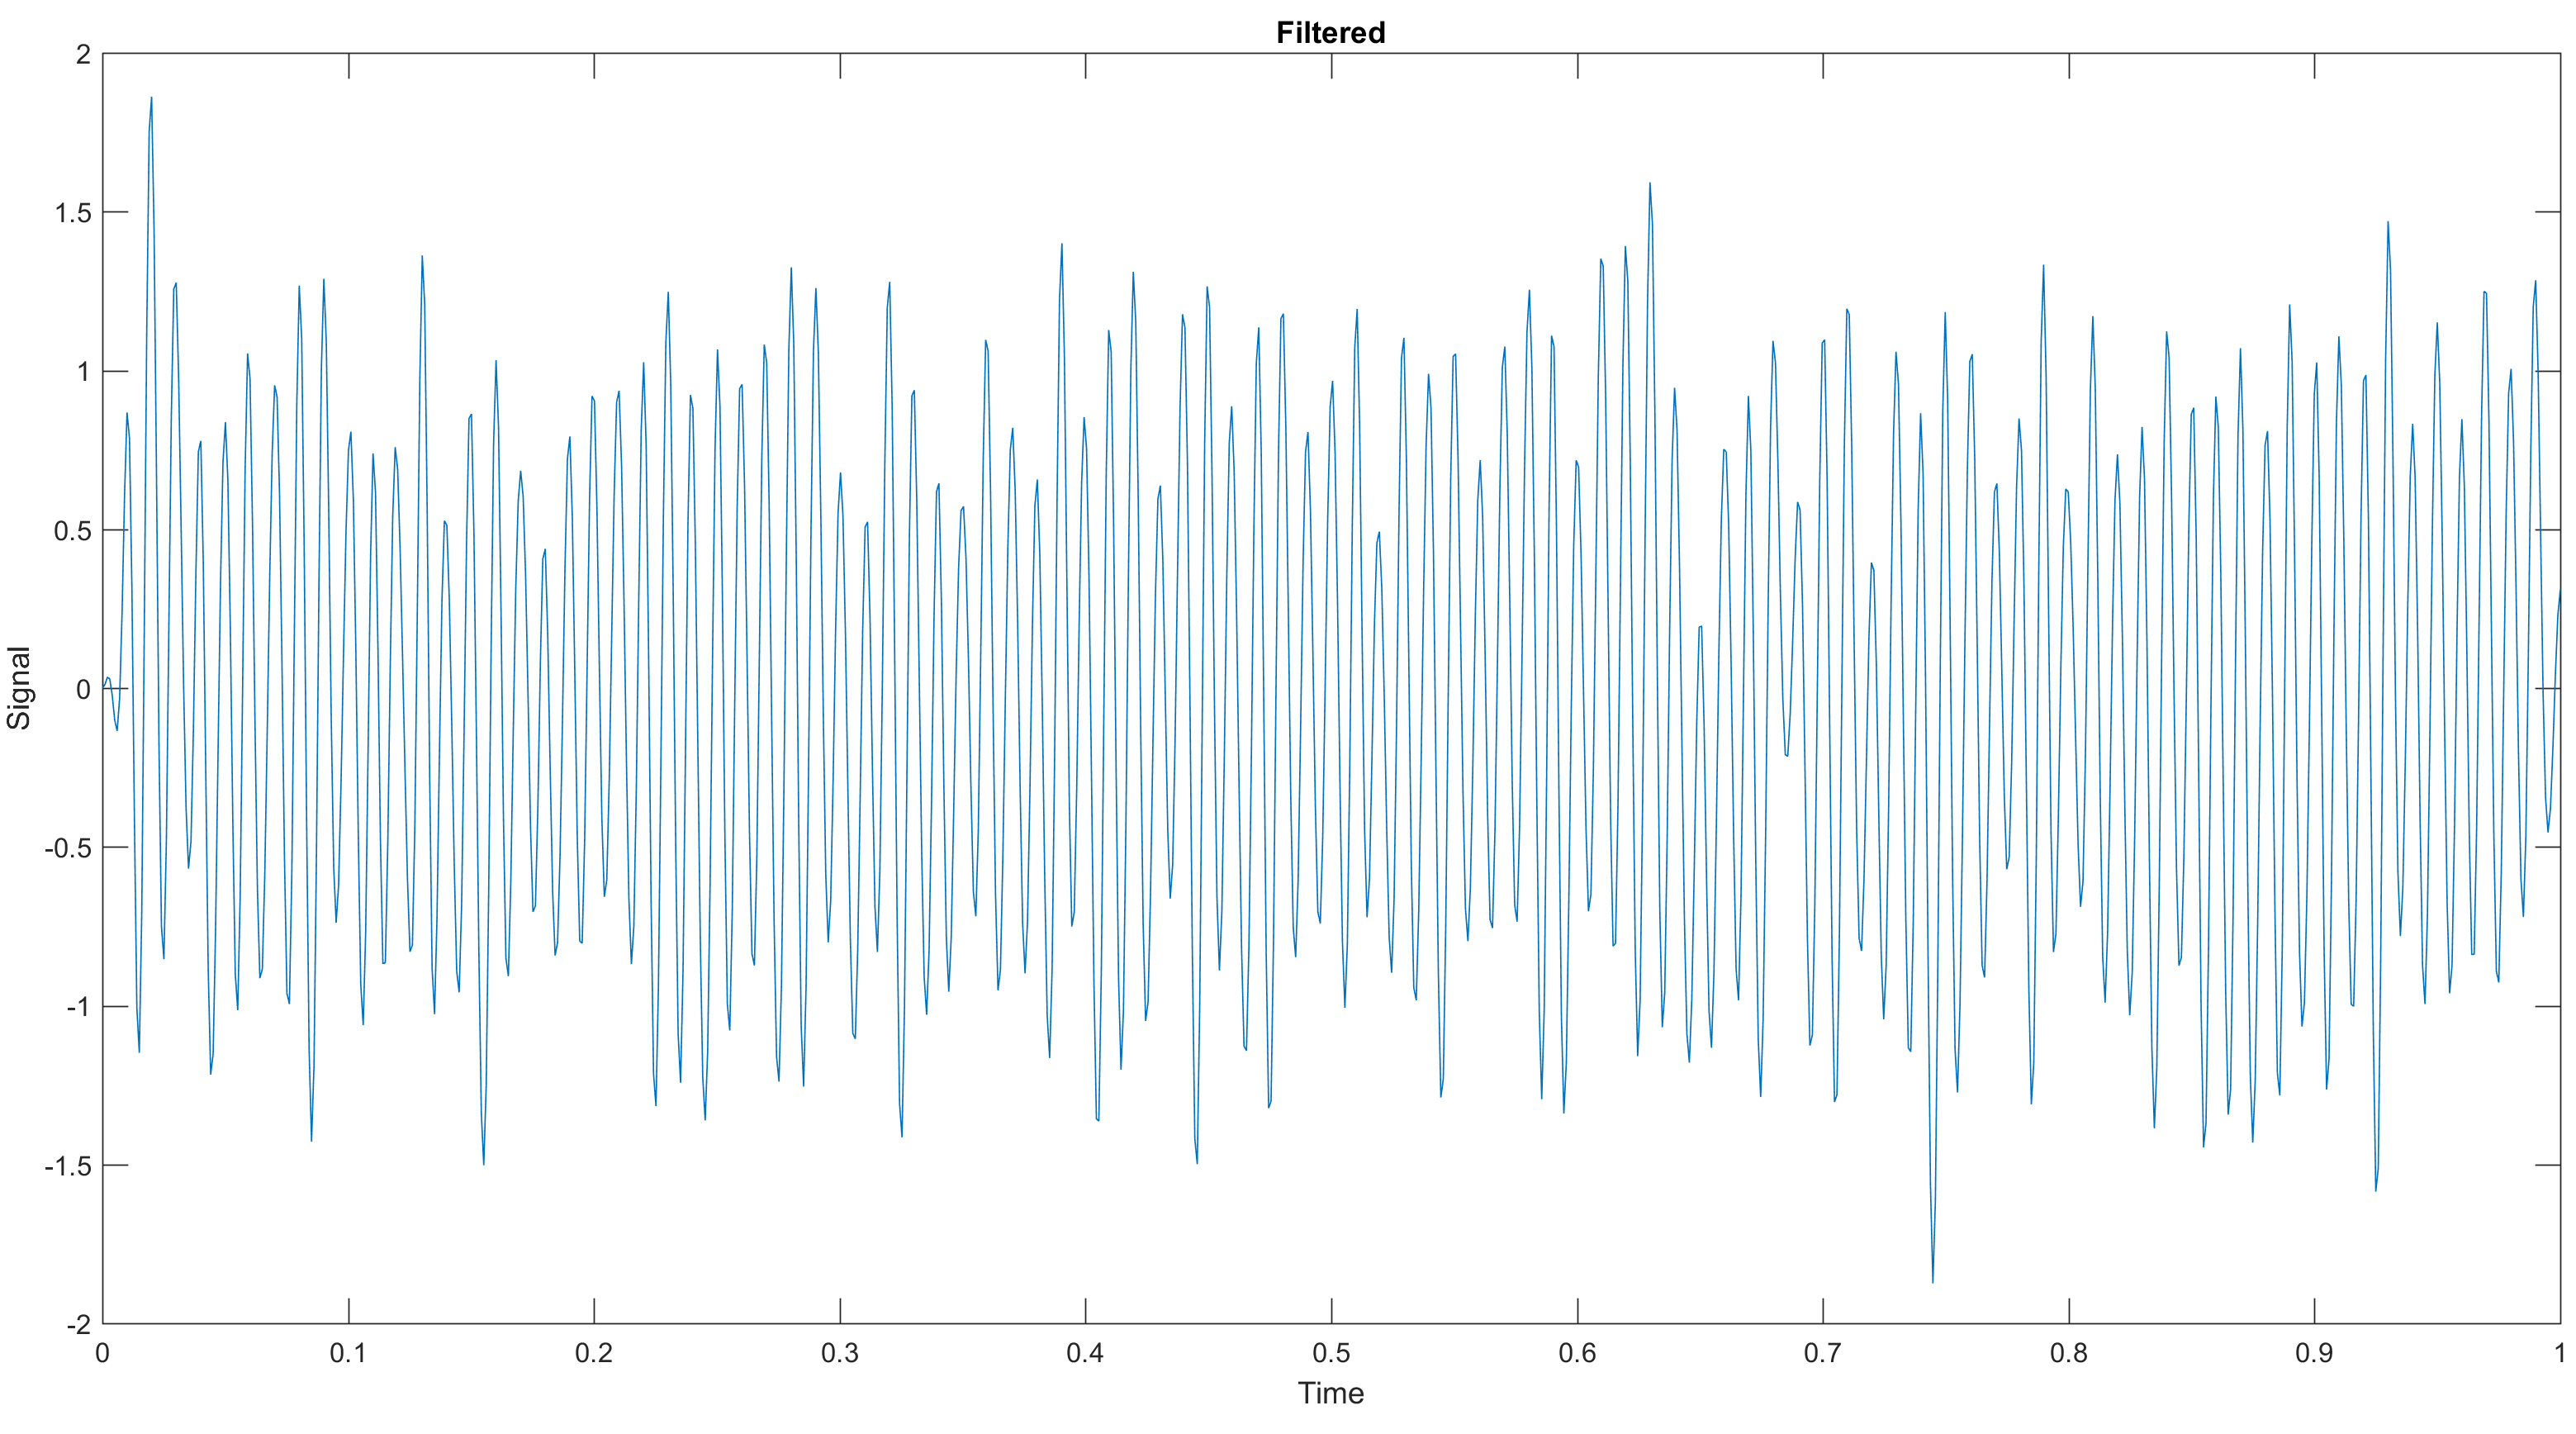
\includegraphics[scale=0.16]{LWPFiltered}}

 \caption{Example of Low Pass Filter}
  \label{fig:Example of Low Pass Filter.}
\end{figure}

\subsubsection{High Pass Filter} \label{ssc:High Pass Filter}
A high-pass attenuates signals below a cutoff frequency (known as the stopband) and passes signals above the cutoff frequency (known as the passband).The amount of attenuation for each frequency depends on the filter design used.  It is the complement of a low-pass filter and they can also be used in conjunction with a low-pass filter to produce a bandpass filter.
\noindent High-pass filters are often used to smooth low-frequency noise and remove low-frequency trends from time series data highlighting the high-frequency trends.
\noindent Common design methods for high-pass FIR-based filters include Kaiser window, least squares, and equiripple. Design methods for IIR-based filters include Butterworth, Chebyshev (Type-I and Type-II), and elliptic.

\noindent Below is shown an example of application of High-Pass-FIR filter on a Signal, with a Sample Rate of $1000$ $Hz$ and a Cutoff Frequency of $150$ $Hz$.


\begin{figure}[H]
\centering	
\subfloat[Filter Response]{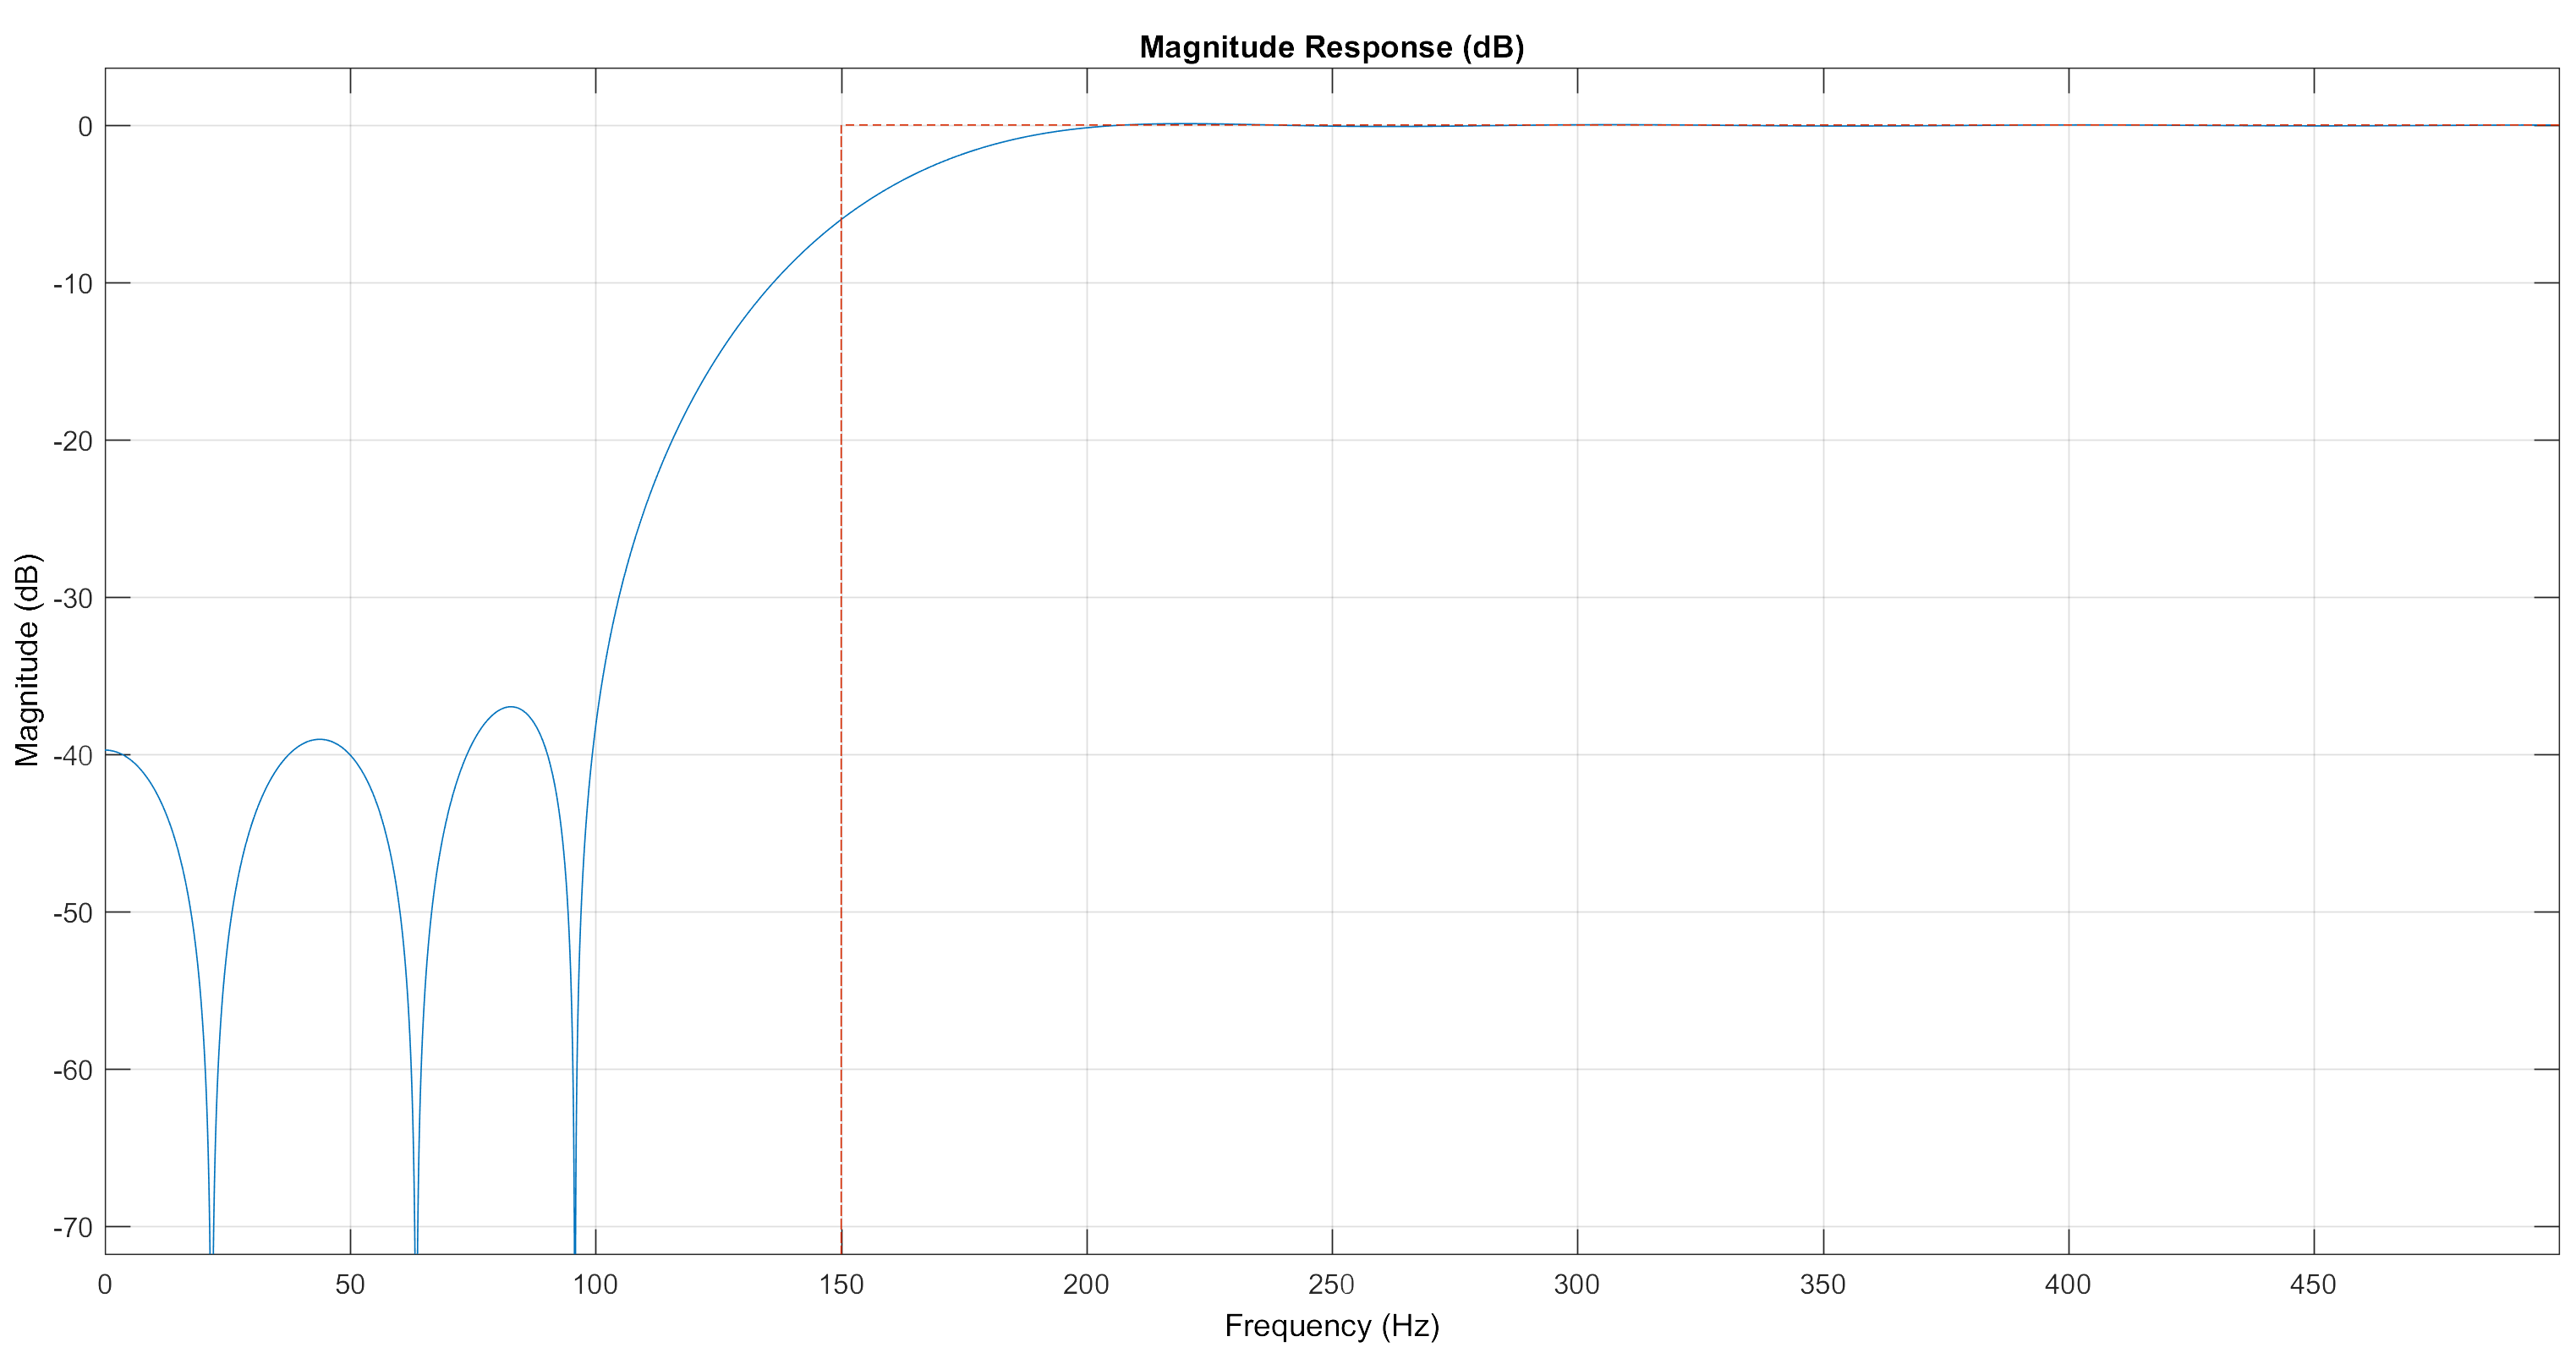
\includegraphics[scale=0.29]{HPFResponse}}    

\subfloat[Unfiltered Signal]{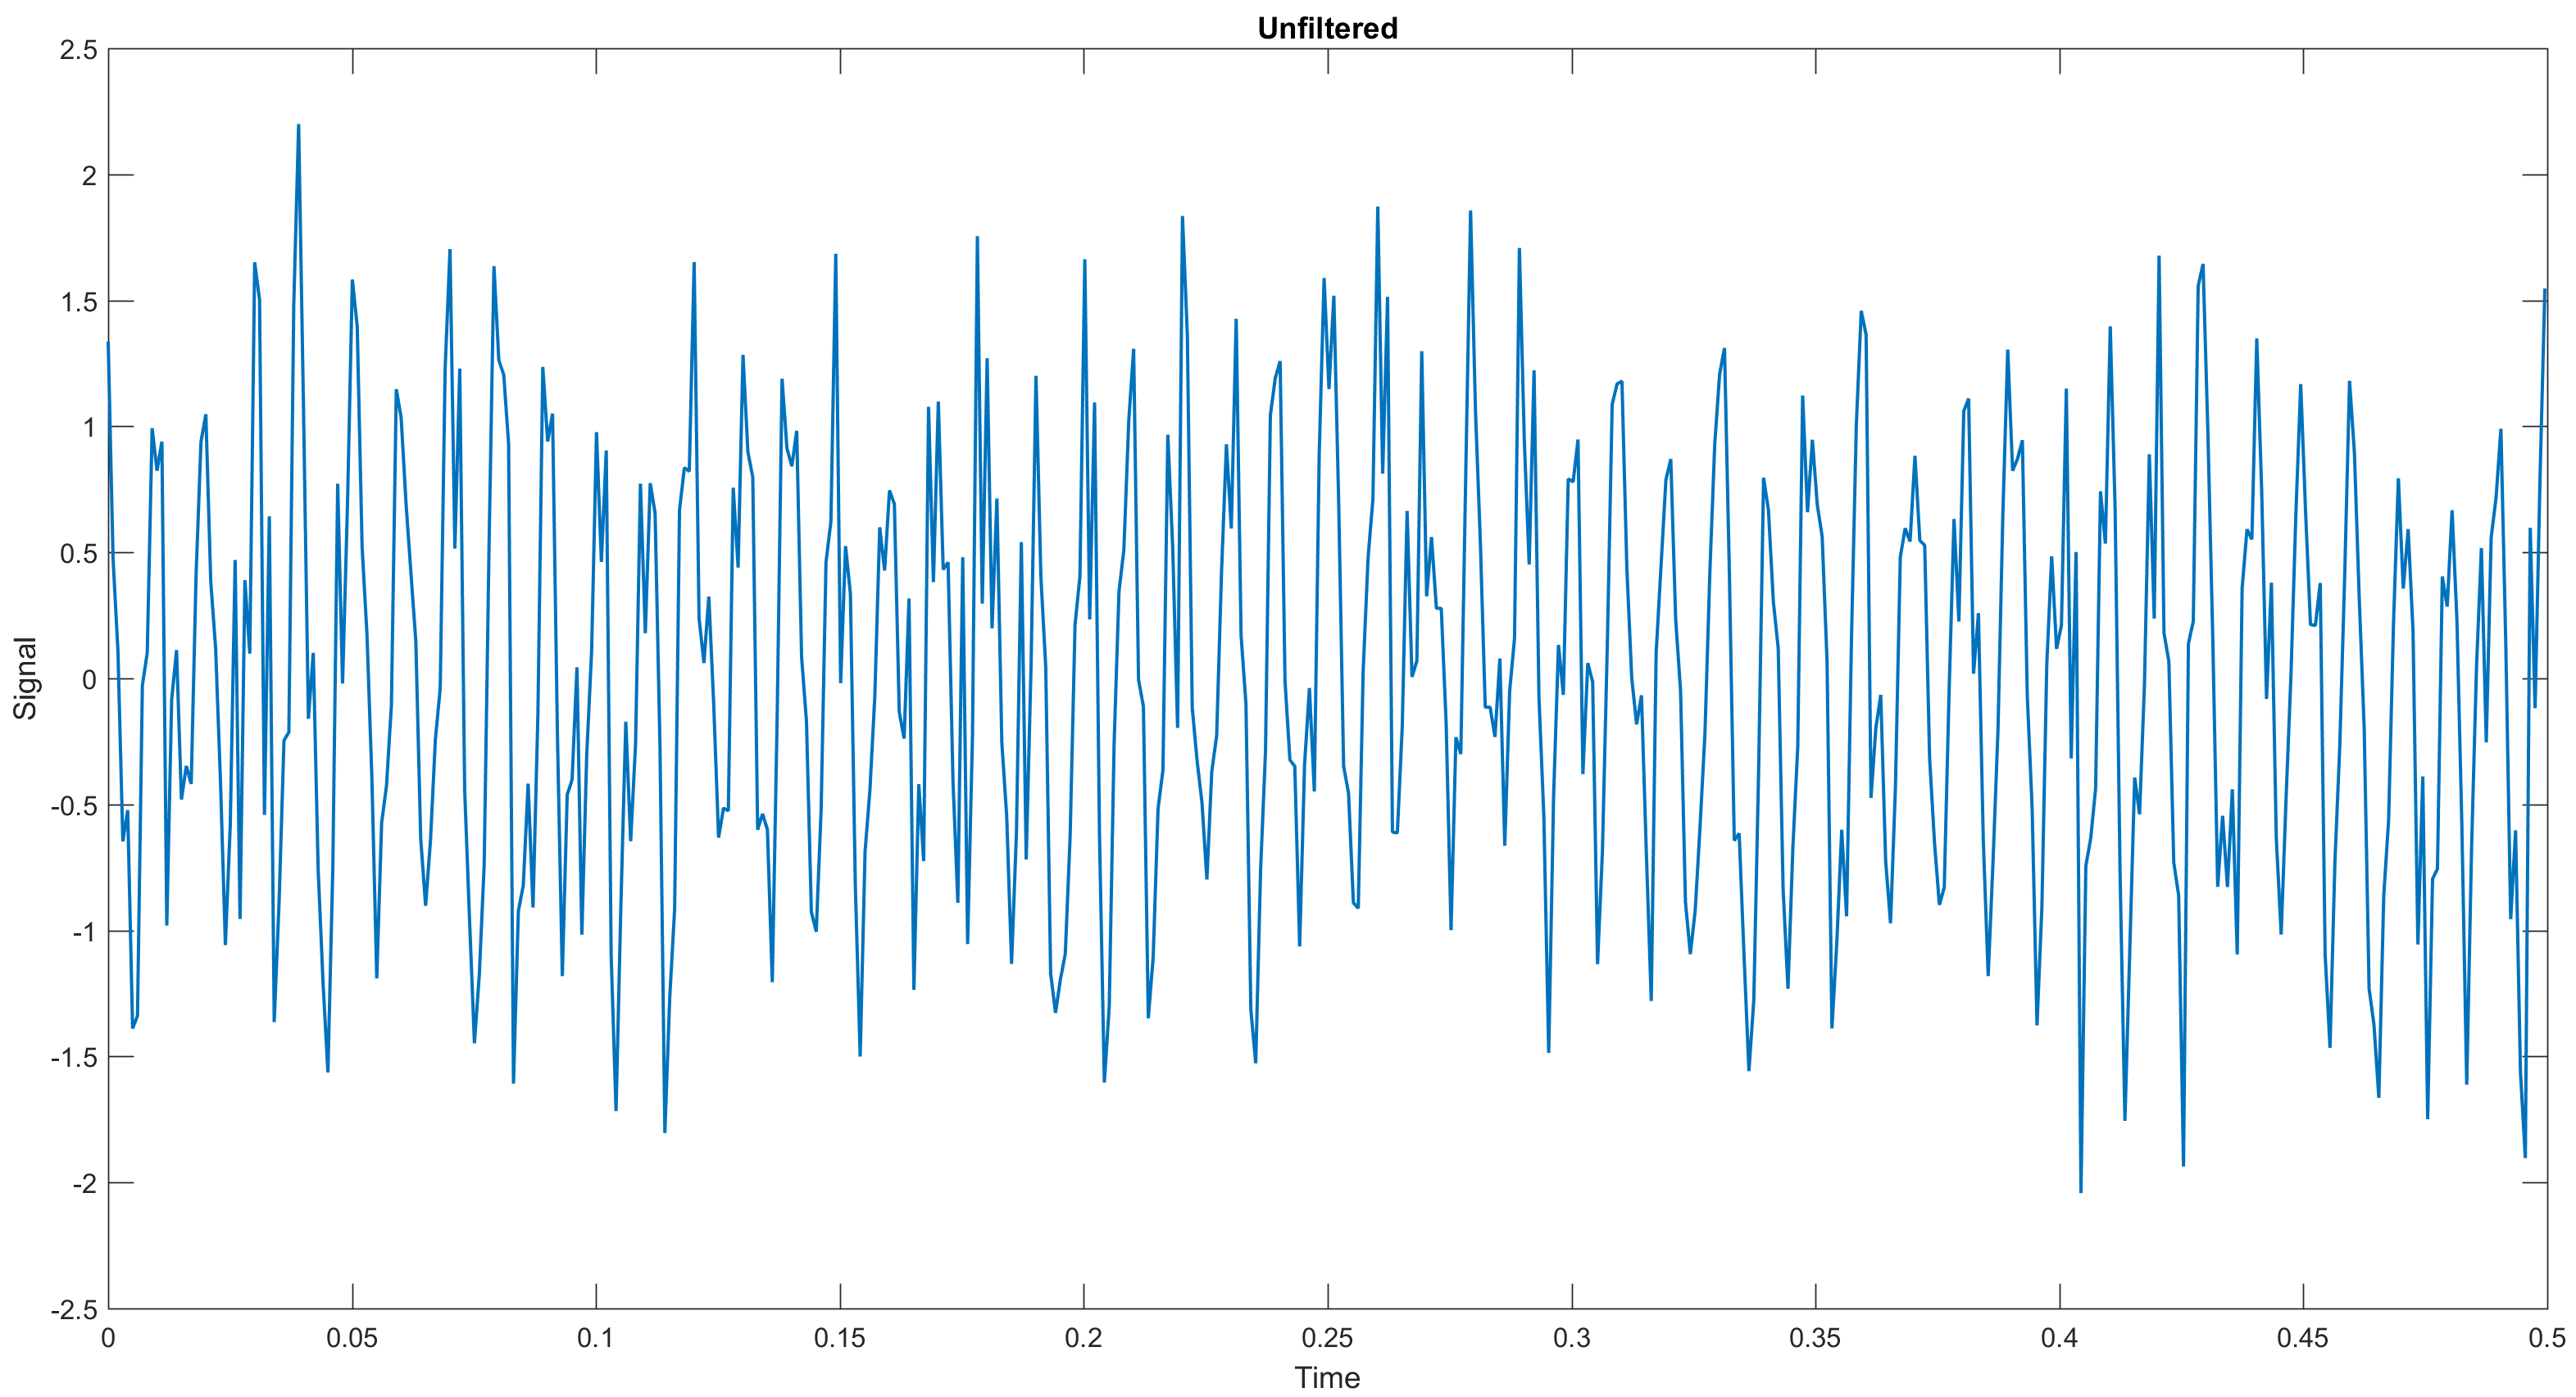
\includegraphics[scale=0.11]{HPFUnfiltered}}
\end{figure}
\begin{figure}[H]
\centering
\subfloat[Filtered Signal]
{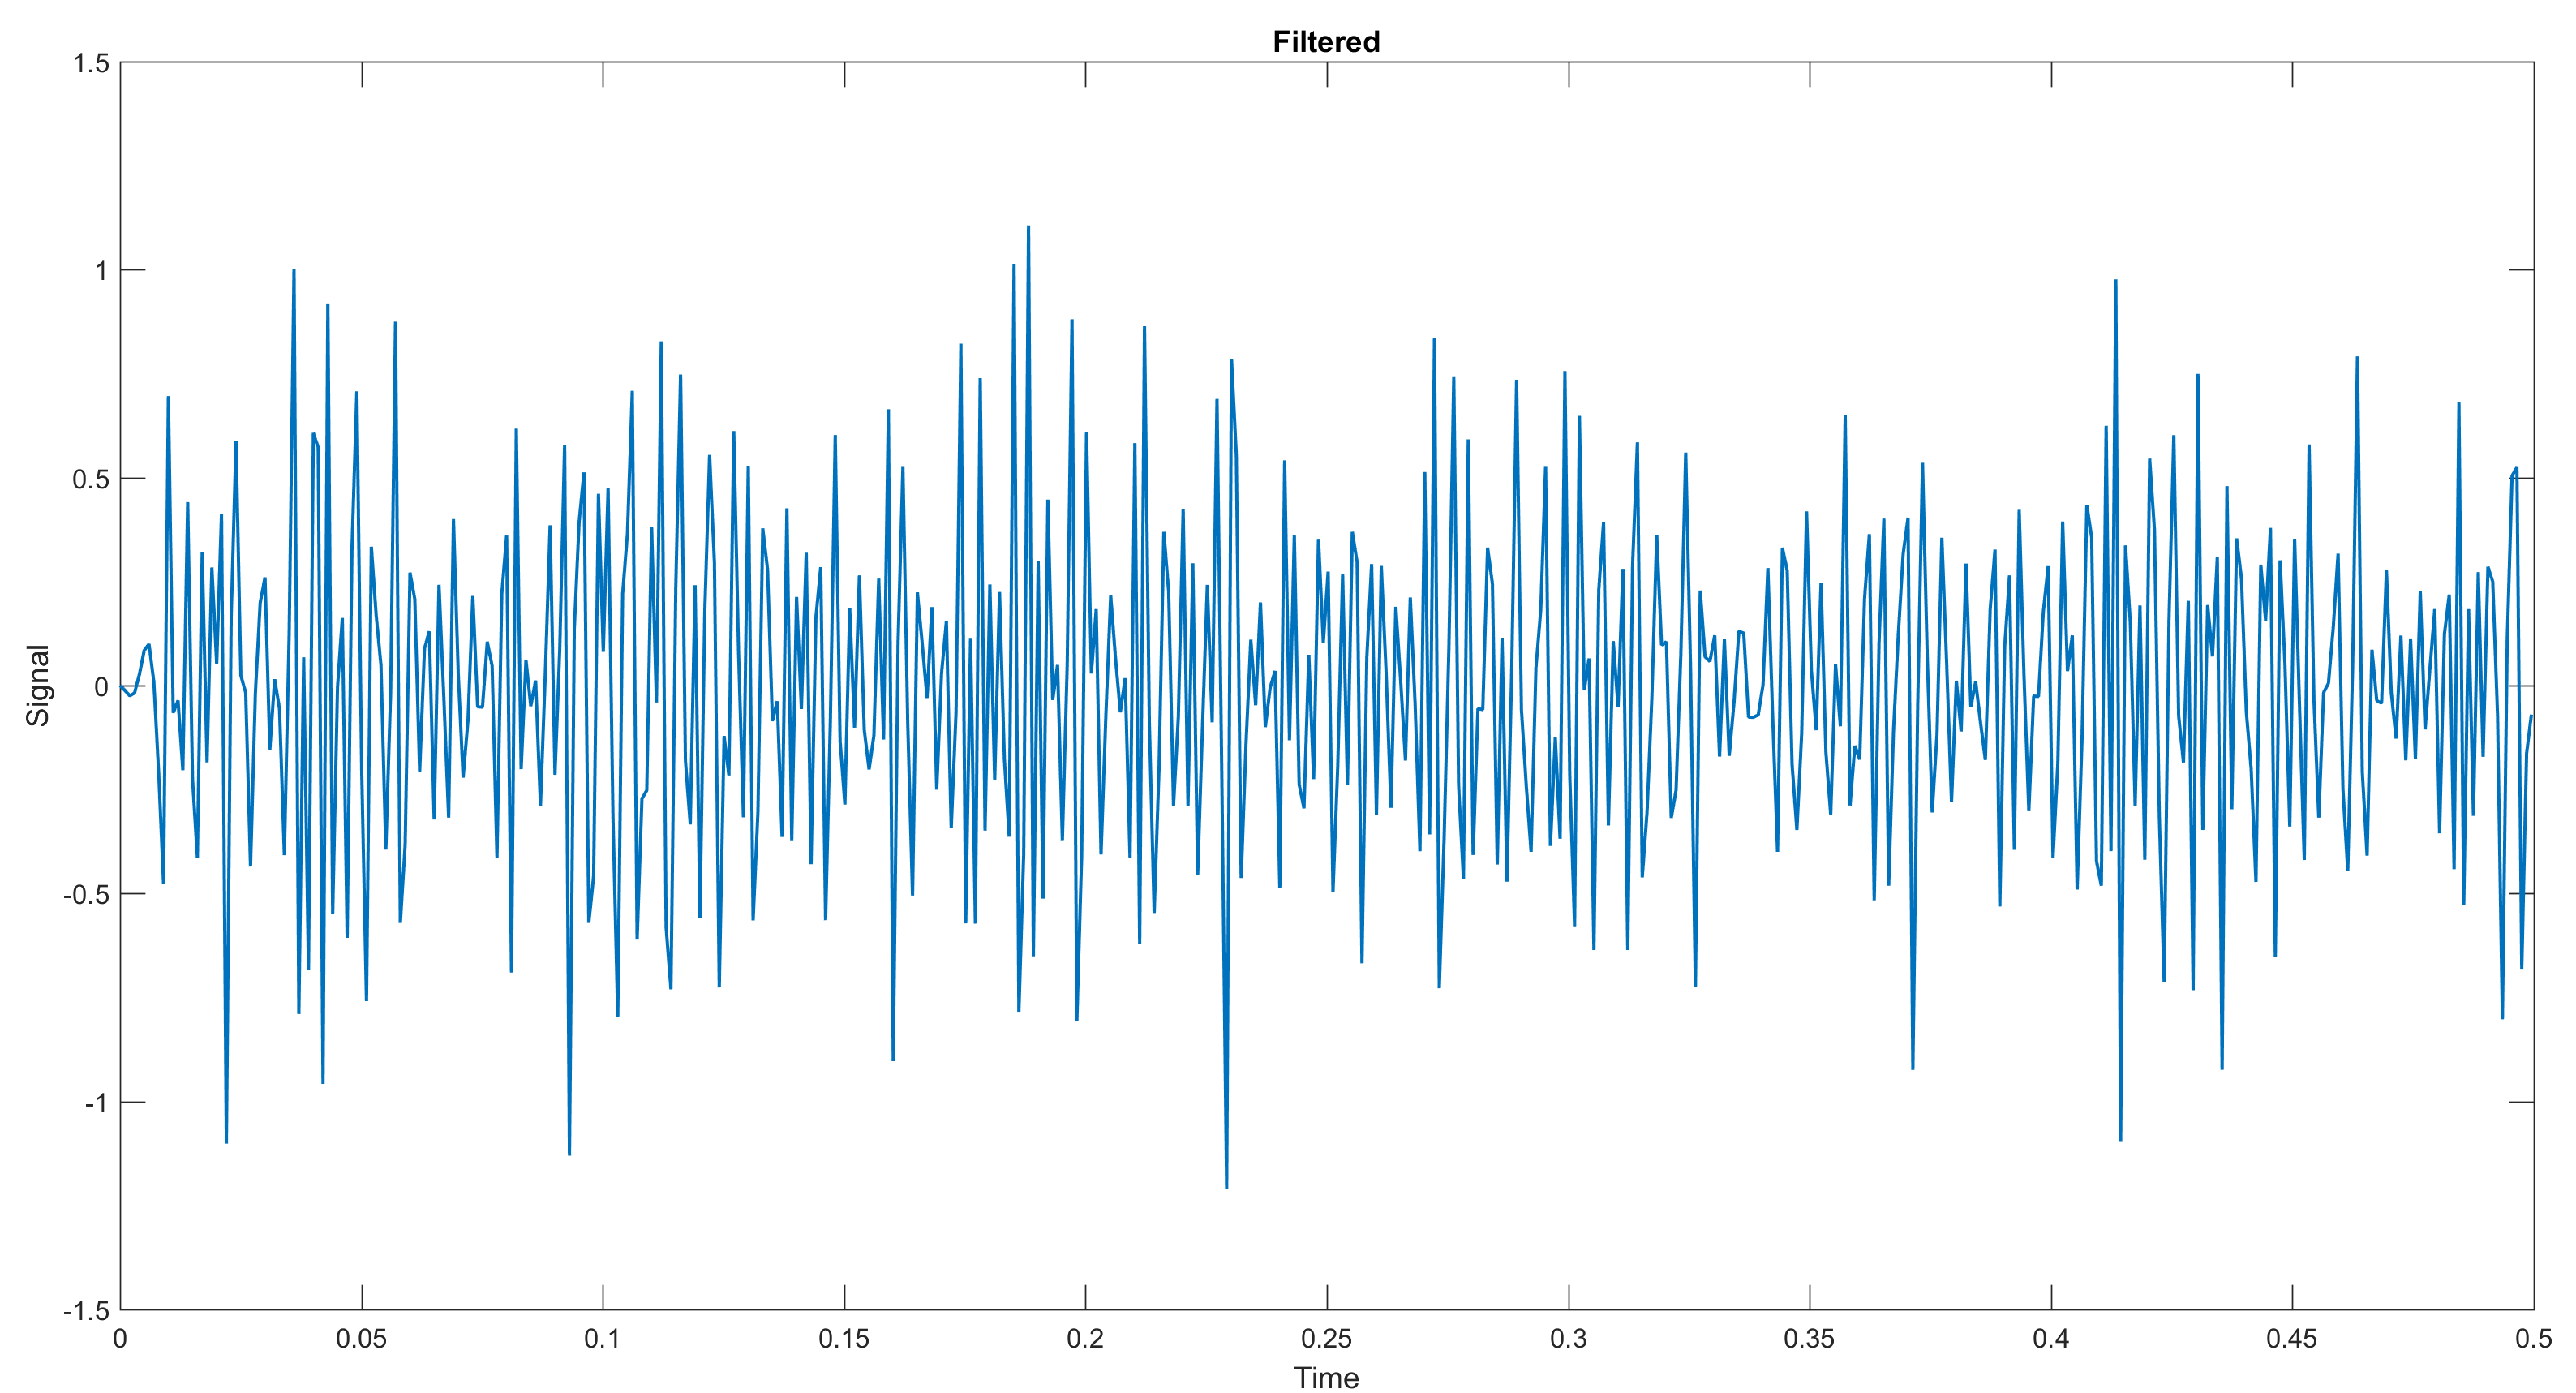
\includegraphics[scale=0.11]{HPFFiltered}}

\subfloat[Signal Overlapping]{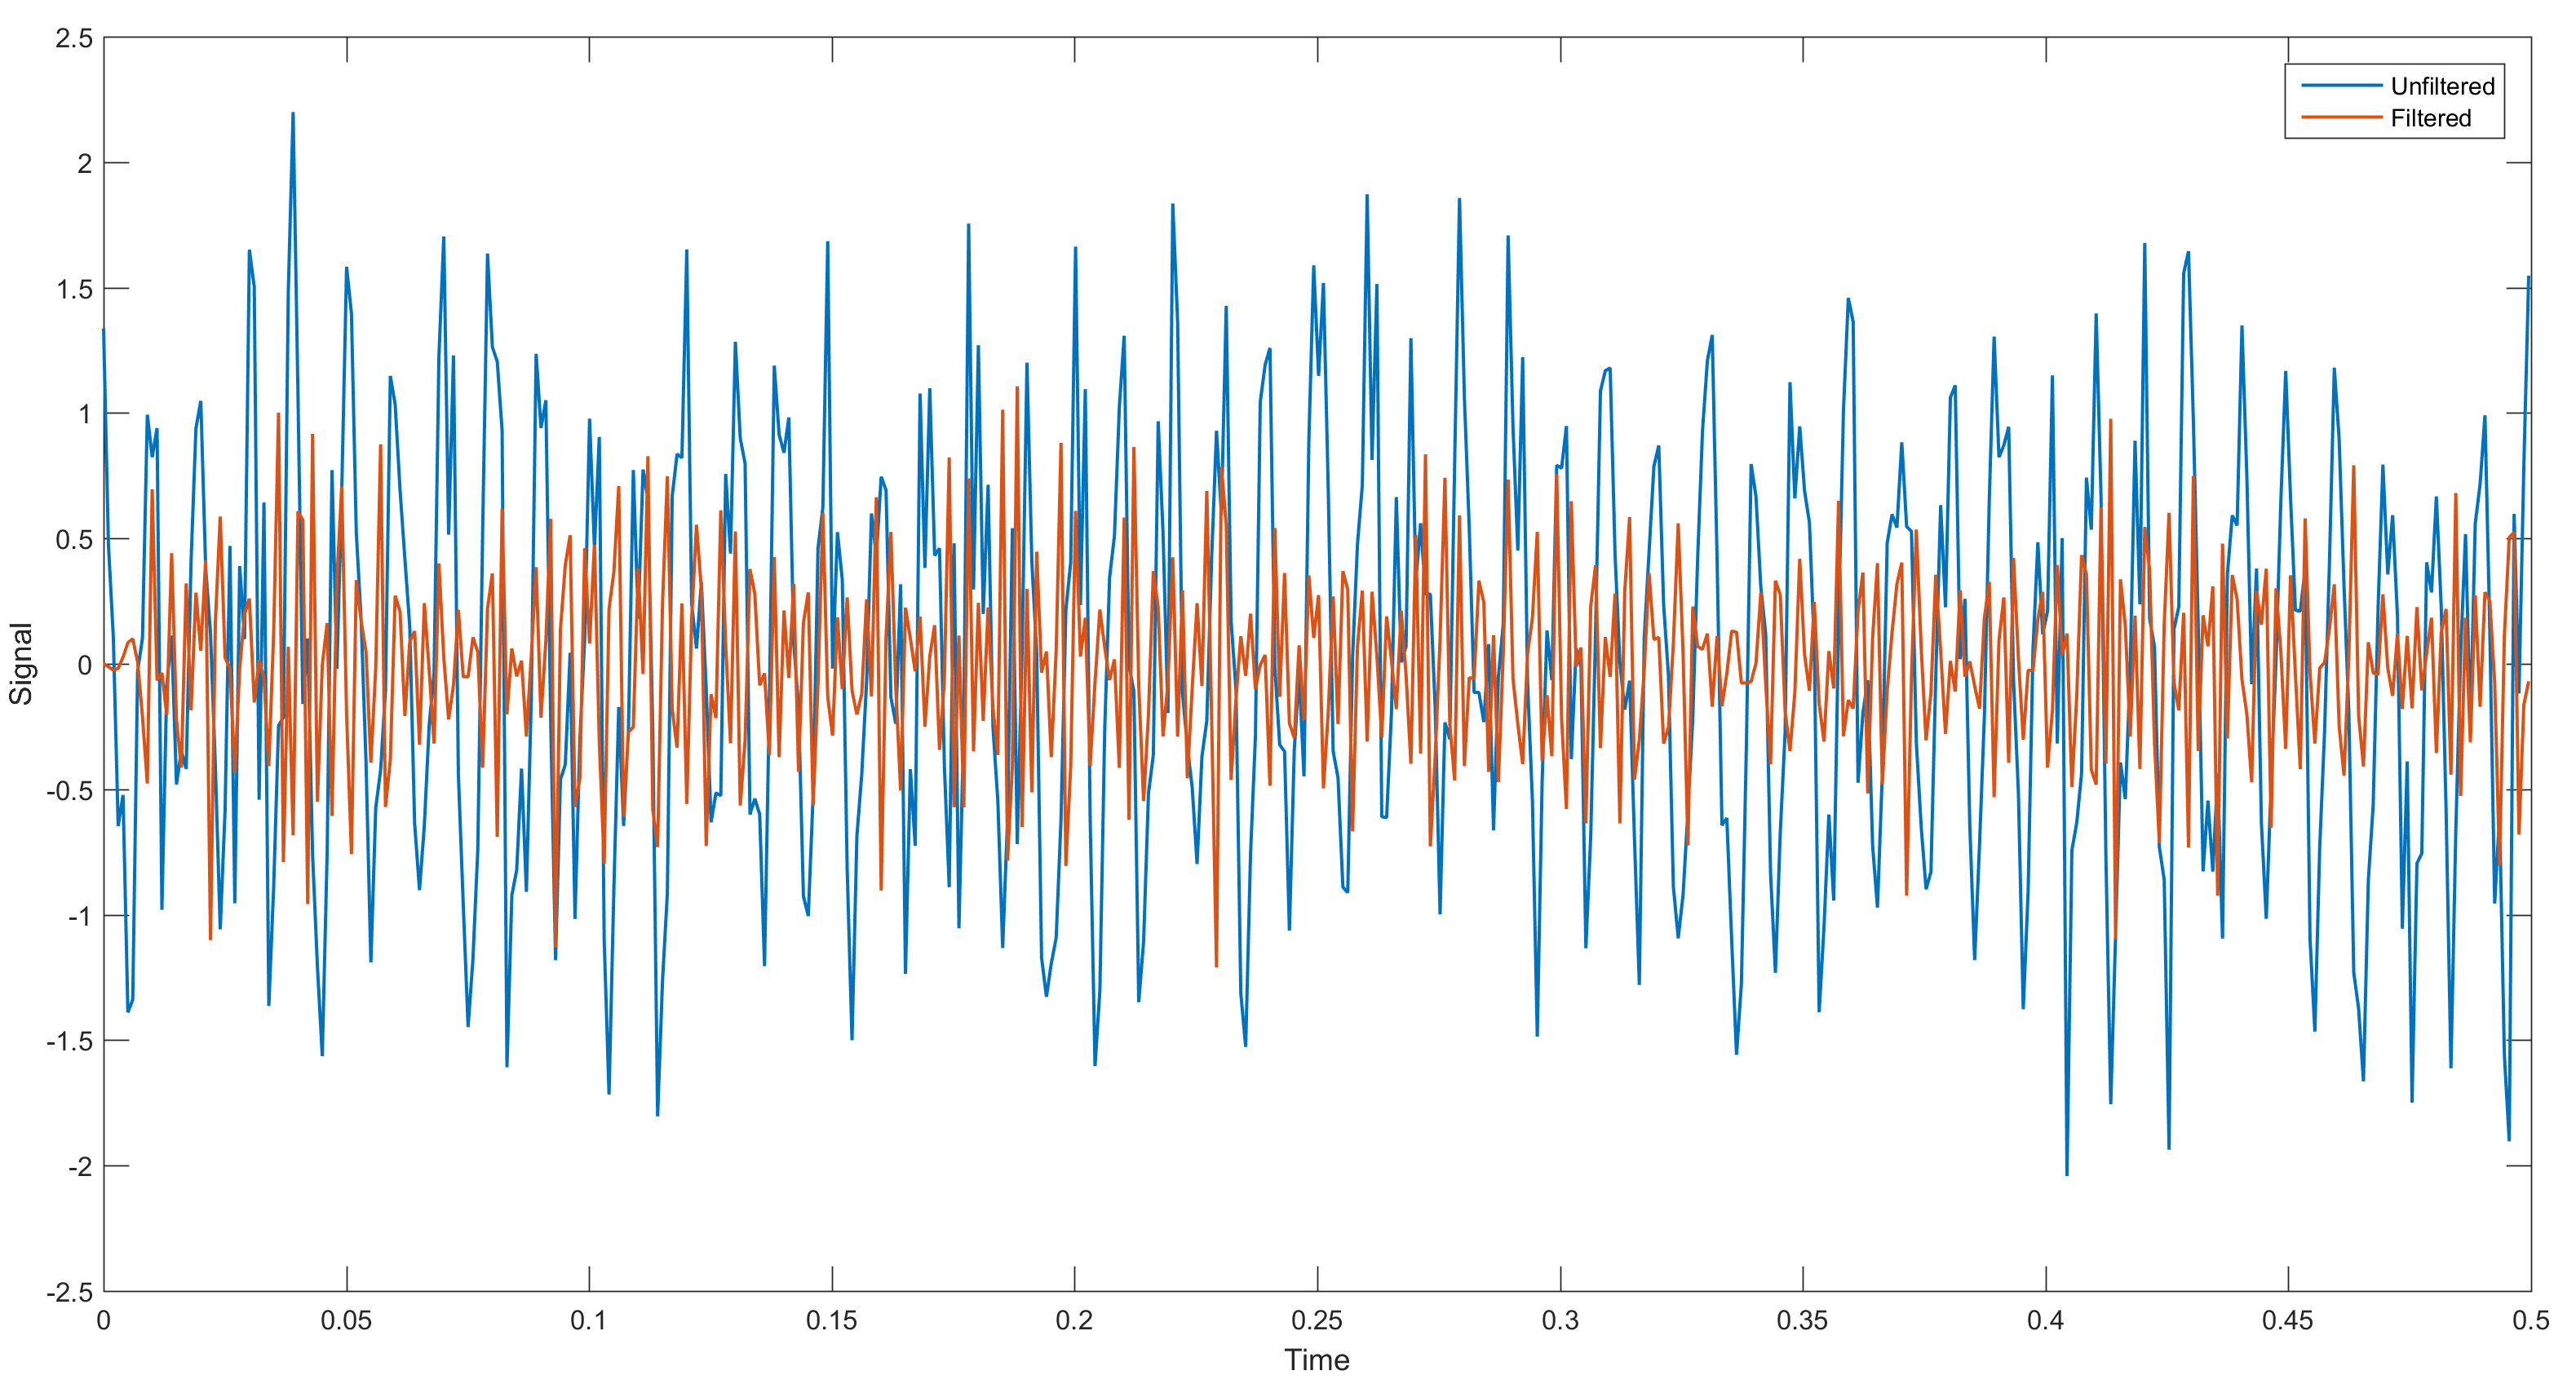
\includegraphics[scale=0.11]{HPFOverlapped}}

The original signal (b) is represent in blue, the filtered signal is represent in orange (c).

 \caption{Example of Application of High Pass Filter}
  \label{fig:Example of Application of Low Pass Filter.}
\end{figure}

\subsubsection{Band Pass Filter} \label{ssc:Band Pass Filter}
A band-pass filter is a filter that passes frequencies within a certain range and attenuates frequencies outside that range. 
The filter can be designed to perform this task by combining the properties of low-pass and high-pass into a single filter.
The ideal band pass filter has a perfectly flat bandpass, does not attenuate the frequencies inside, and completely attenuates all frequencies outside of this range.
In practice, no band pass filter is ideal. The filter does not completely attenuate all frequencies outside the desired bandwidth.
Between the lower frequency $f_{1}$ and the higher $f_{2}$ of a band pass, is located the resonance frequency, in which the filter gain is maximum. 
The filter's bandpass is simply the difference between $f_{2}$ and $f_{1}$. 

Below is shown an example of the Response of a Band Pass Filter with lower frequency $f_{1} \thinspace = \thinspace 250 \thinspace Hz$ and higher frequency $f_{2} \thinspace = \thinspace 550 \thinspace Hz$. 

\begin{figure}[H]
\centering
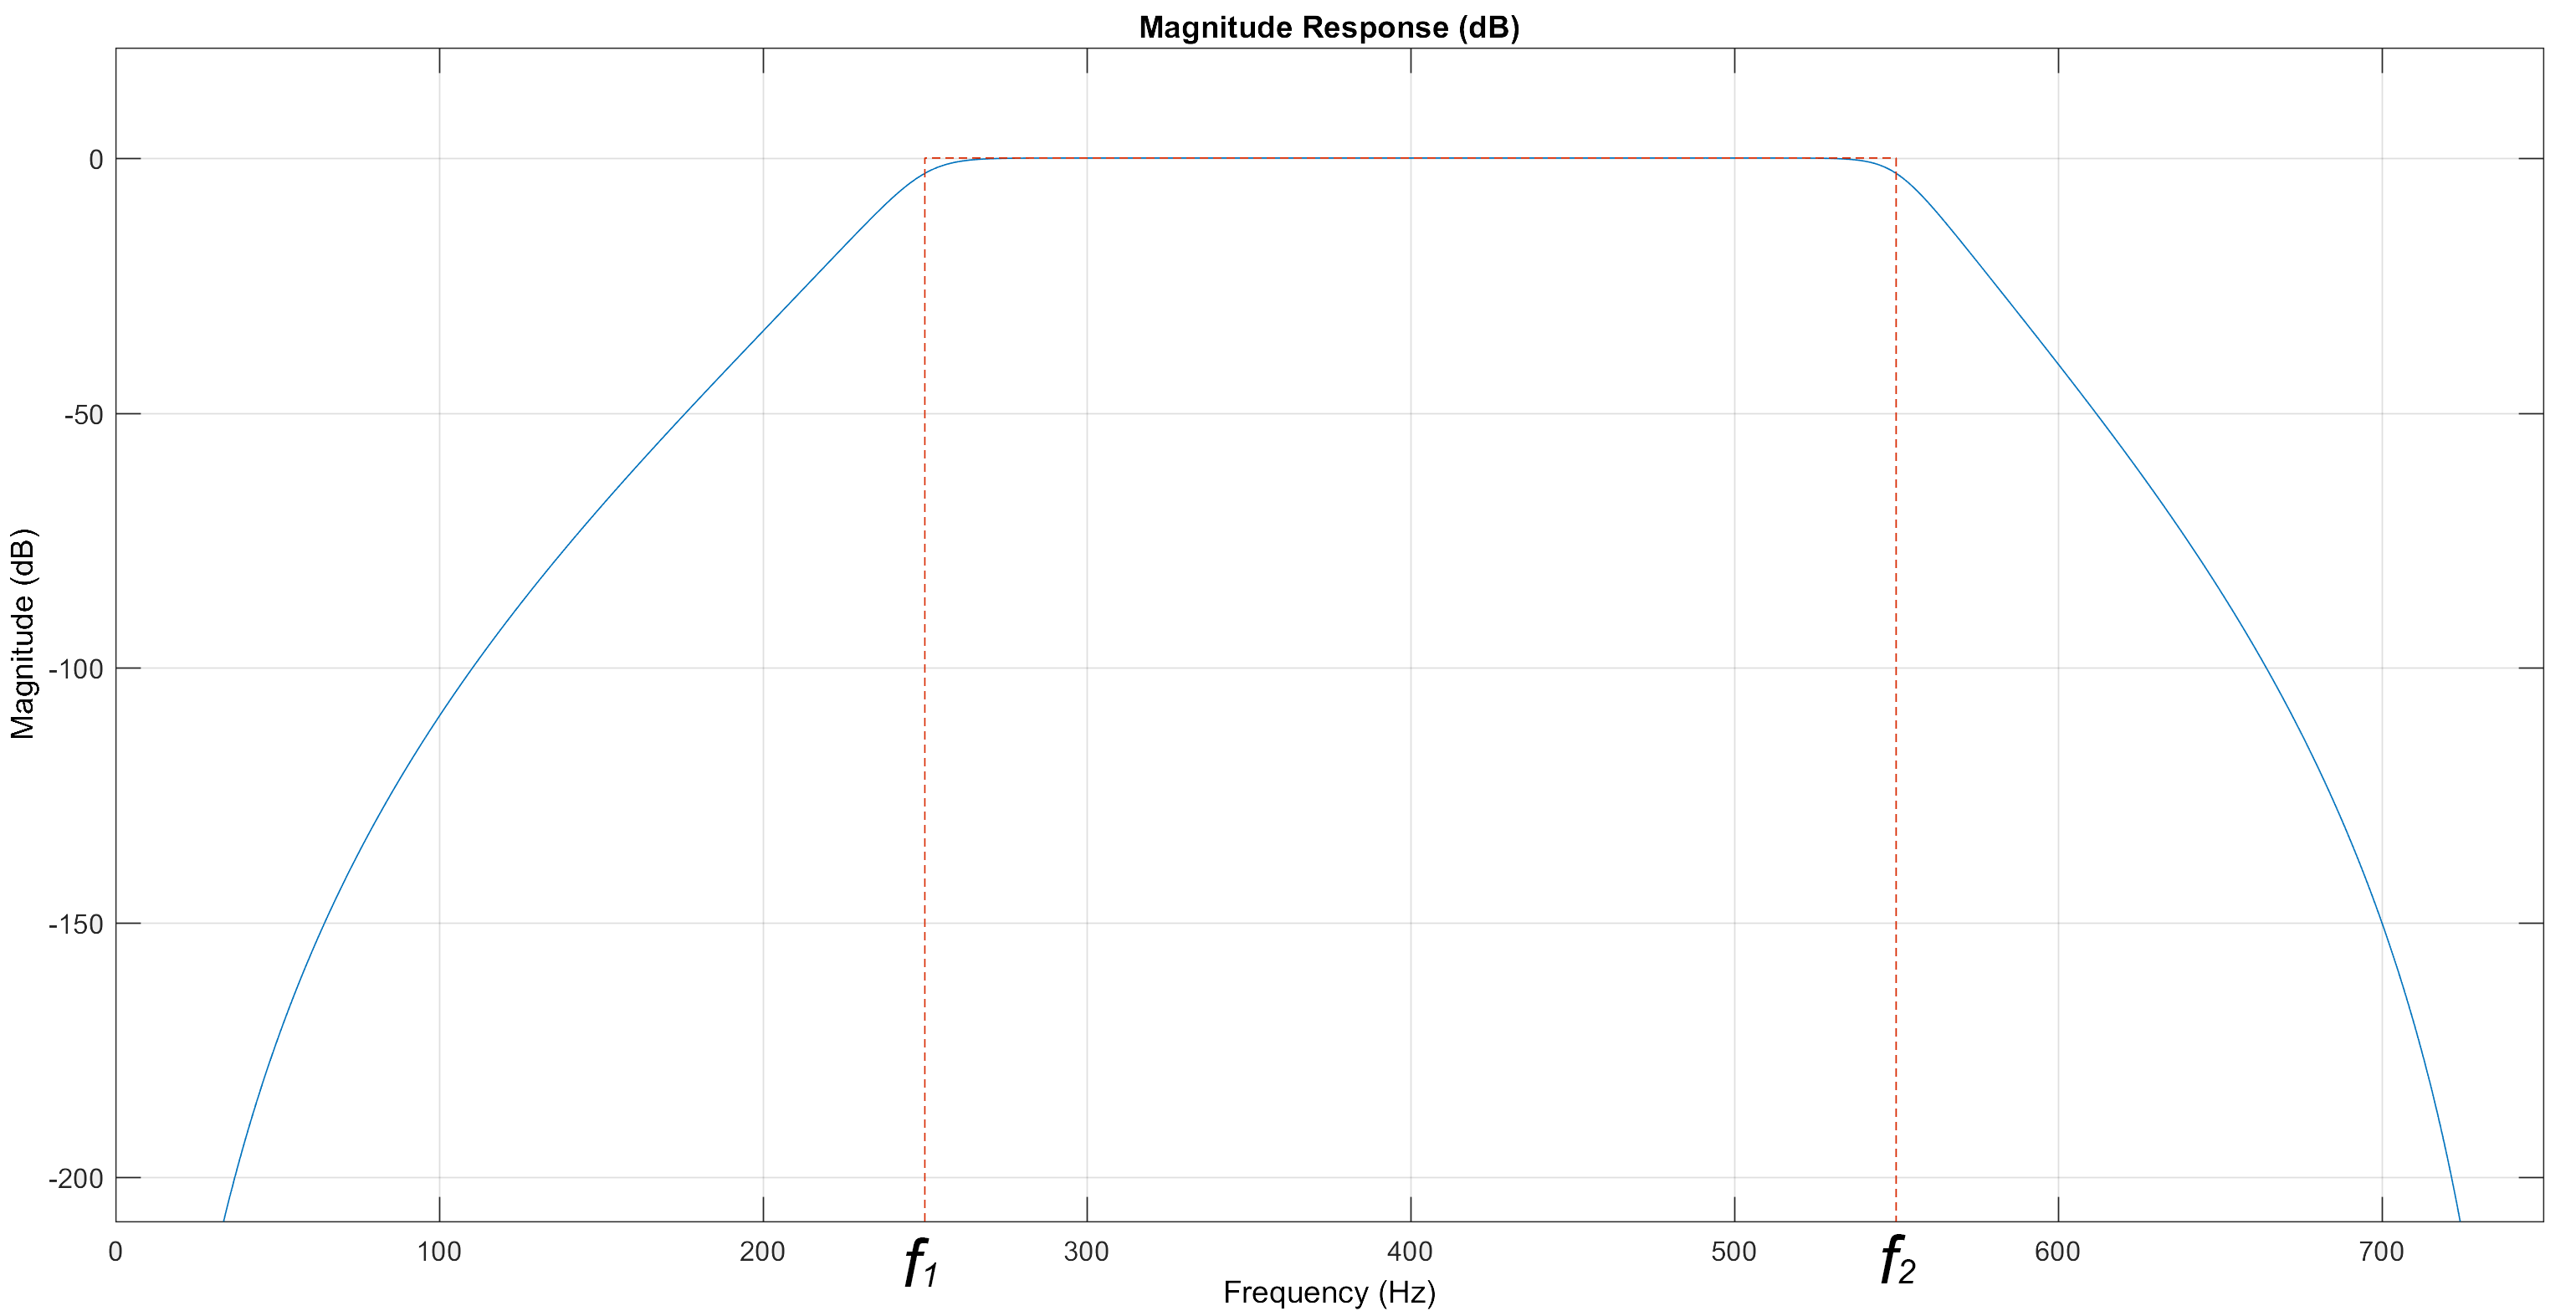
\includegraphics[scale=0.45]{BPFResponse} 
 \caption{Band Pass Filter Response}
  \label{fig:Band Pass Filter Response}
\end{figure}
\section{Fast Fourier Transform} \label{sc:Fast Fourier Transform}
Various data filtering techniques have been analysed but in order to understand in which frequencies we find the signal disturbance, and so choose the cutoff frequency properly the Fourier Transform can be used.
The Fourier Transform is a mathematical technique widely used in science, engineering and digital signal processing. 
The mathematical technique called the Discrete Fourier Transform (DFT) takes a discrete time series of $n$ equally spaced numbers and transforms or converts this time series through a mathematical operation into a set of $n$ complex numbers defined into the frequency domain from the time domain. 
DFT is an extremely powerful mathematical tool that allows to view signals in a different domain, inside which several difficult problems become very simple to analyse respect the original time series, in which is computationally is hard to do.
If the time series is made up of oscillating signals of various frequencies plus noise, in the frequency domain we can found frequencies we have no interest and also found the noise content of the price data.

To check this, compute the DFT m of Signal and see what it looks like in the frequency domain. The Fast Fourier Transform (FFT) is a mathematical algorithm that computes the DFT very fast.
The DFT formula:
\begin{equation}
X(m\omega_{s})\thinspace = \sum\limits_{k=0}^{N- 1} x_{k} e^{-jm\omega_{s}k}
\quad where \quad \omega_{s} = \dfrac{2\pi}{N}
\end{equation}\label{eq:dft}
\noindent Computed this it is possible to see if a spectral peak is present. For this purpose, MATLAB has the $fft$ function, which performs the DFT computation\ref{eq:dft} in an efficient manner, it is called the Fast Fourier Transform (FFT). Hand it a vector $x$ of time domain samples, and it returns a vector $X$ of samples $X(m\omega_{s}),\thinspace m = 0, 1,..., N-  1$ of the DFT computation.
If we take for example this signal:
\begin{figure}[H]
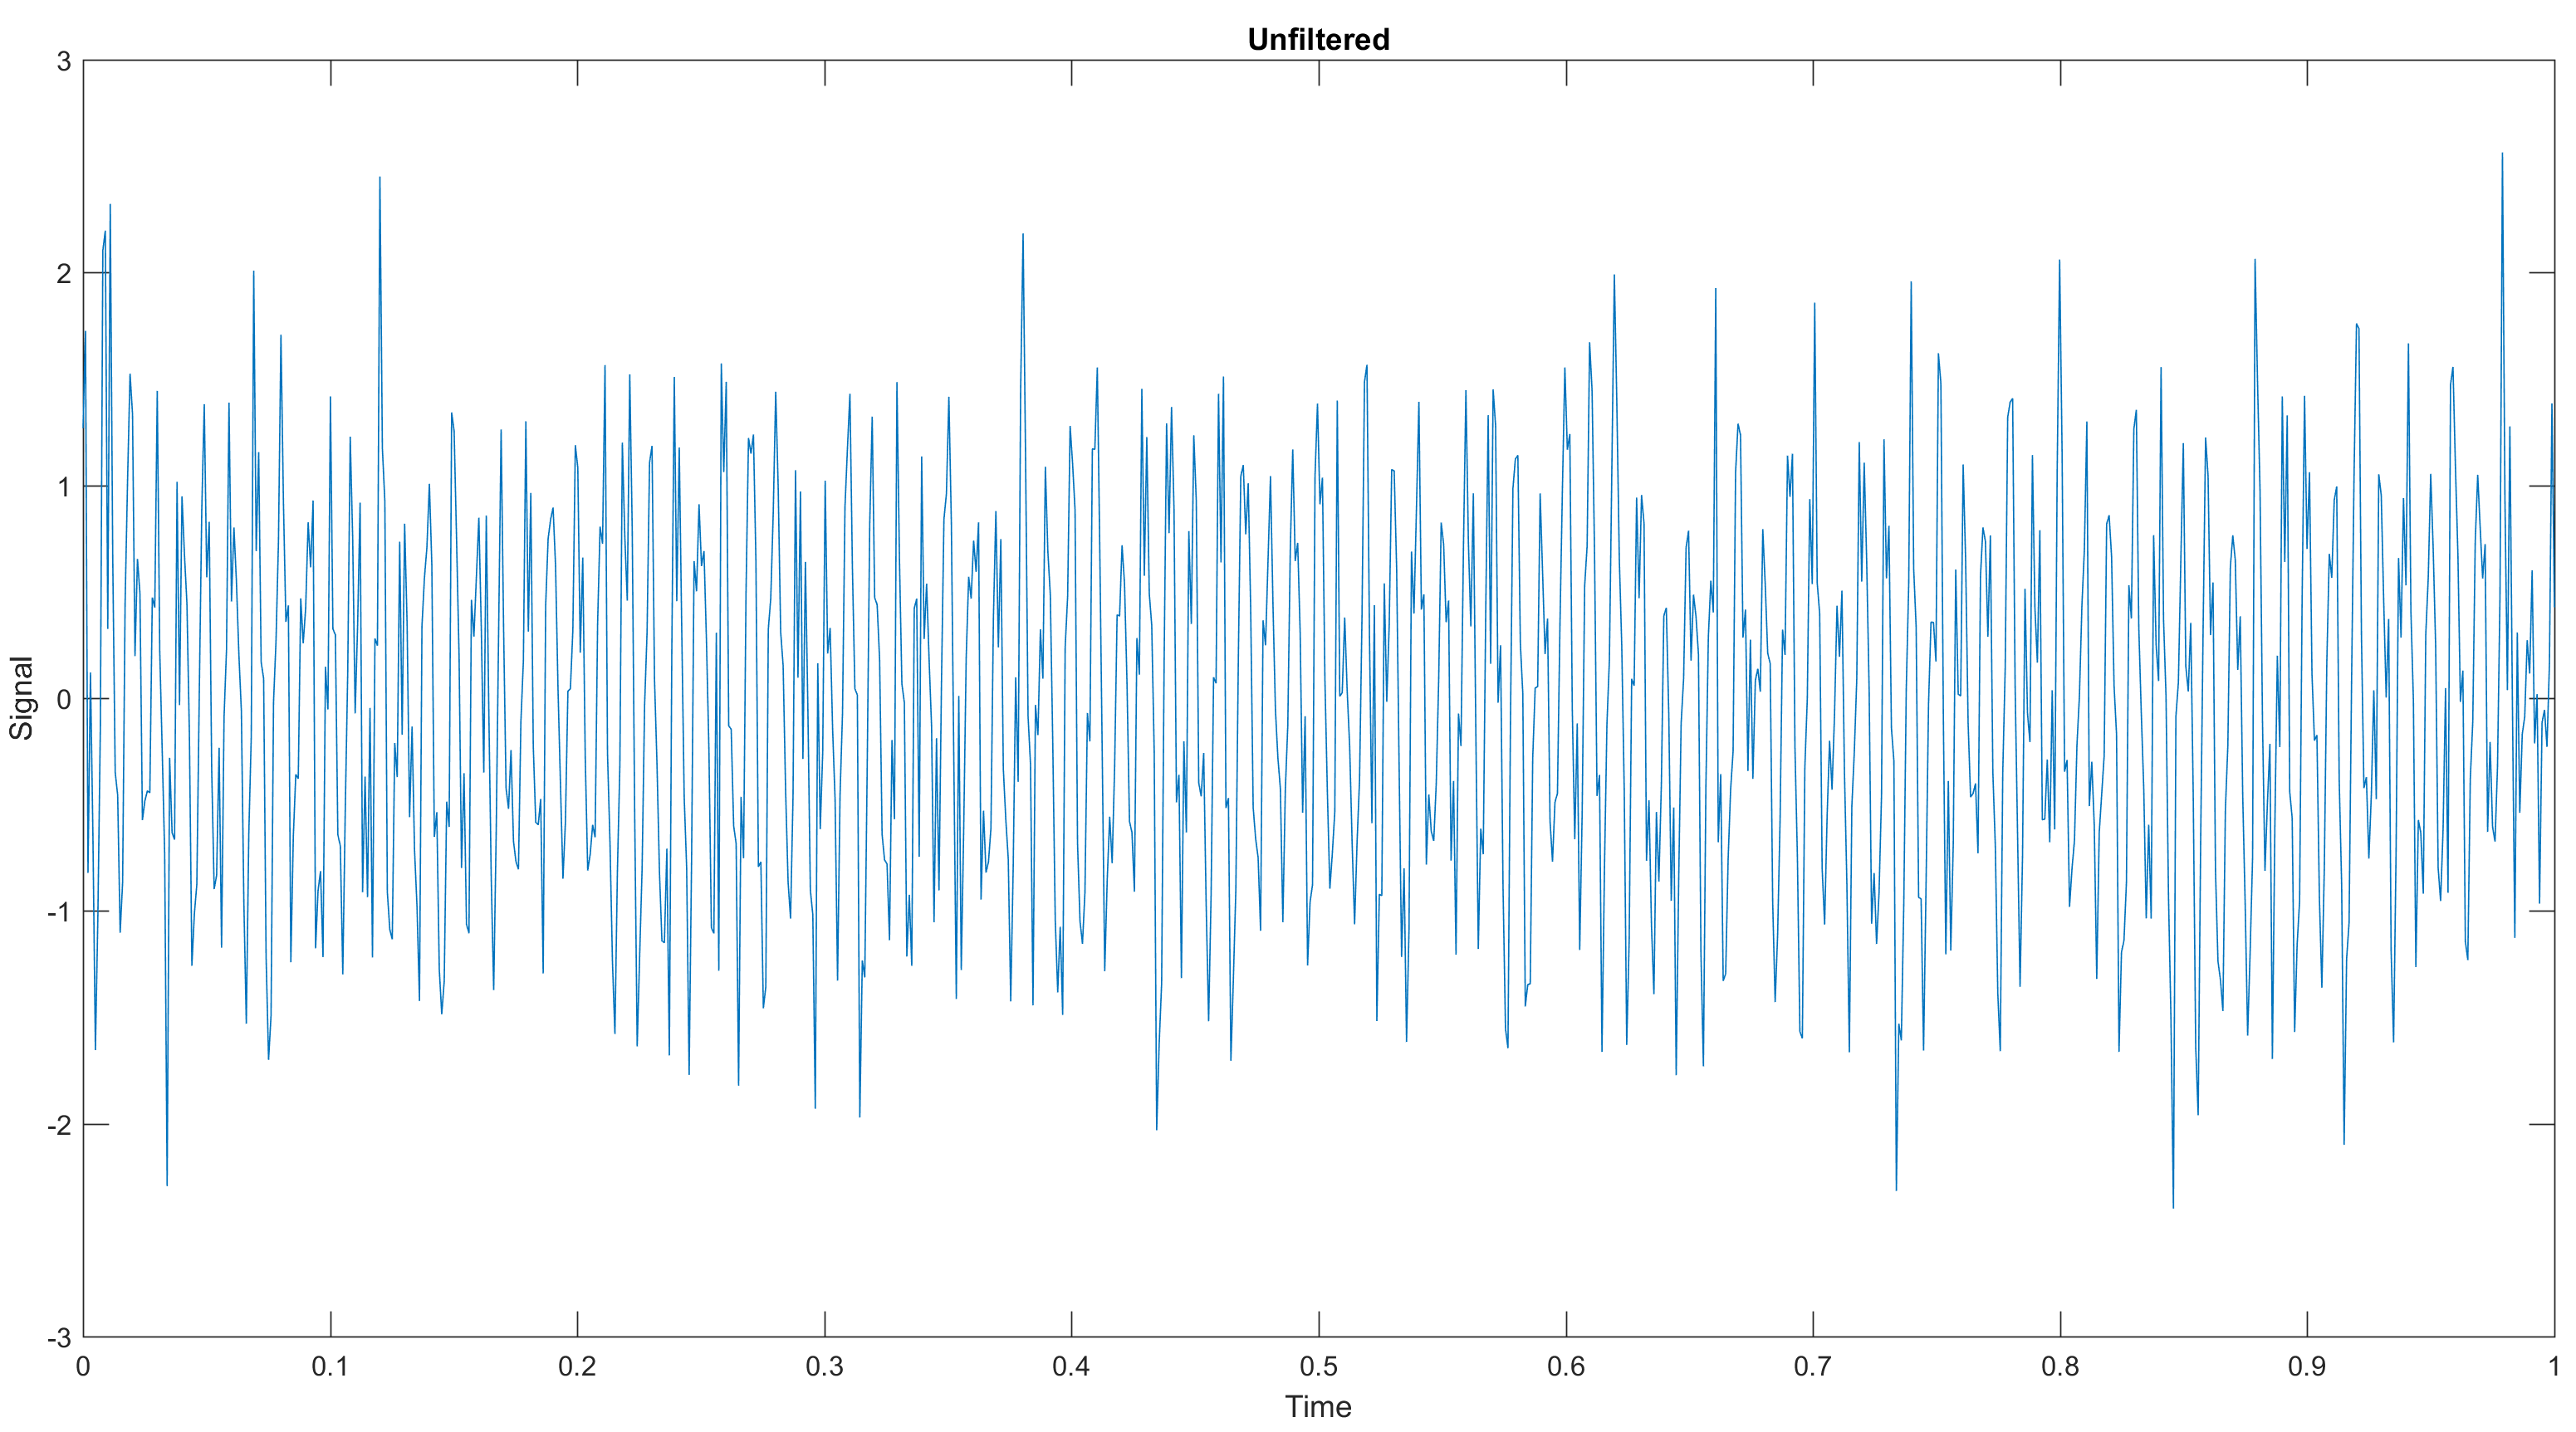
\includegraphics[scale=0.16]{LWPUnfitltered}
\end{figure}
\noindent And compute the $fft$:
\begin{figure}[H]
\centering
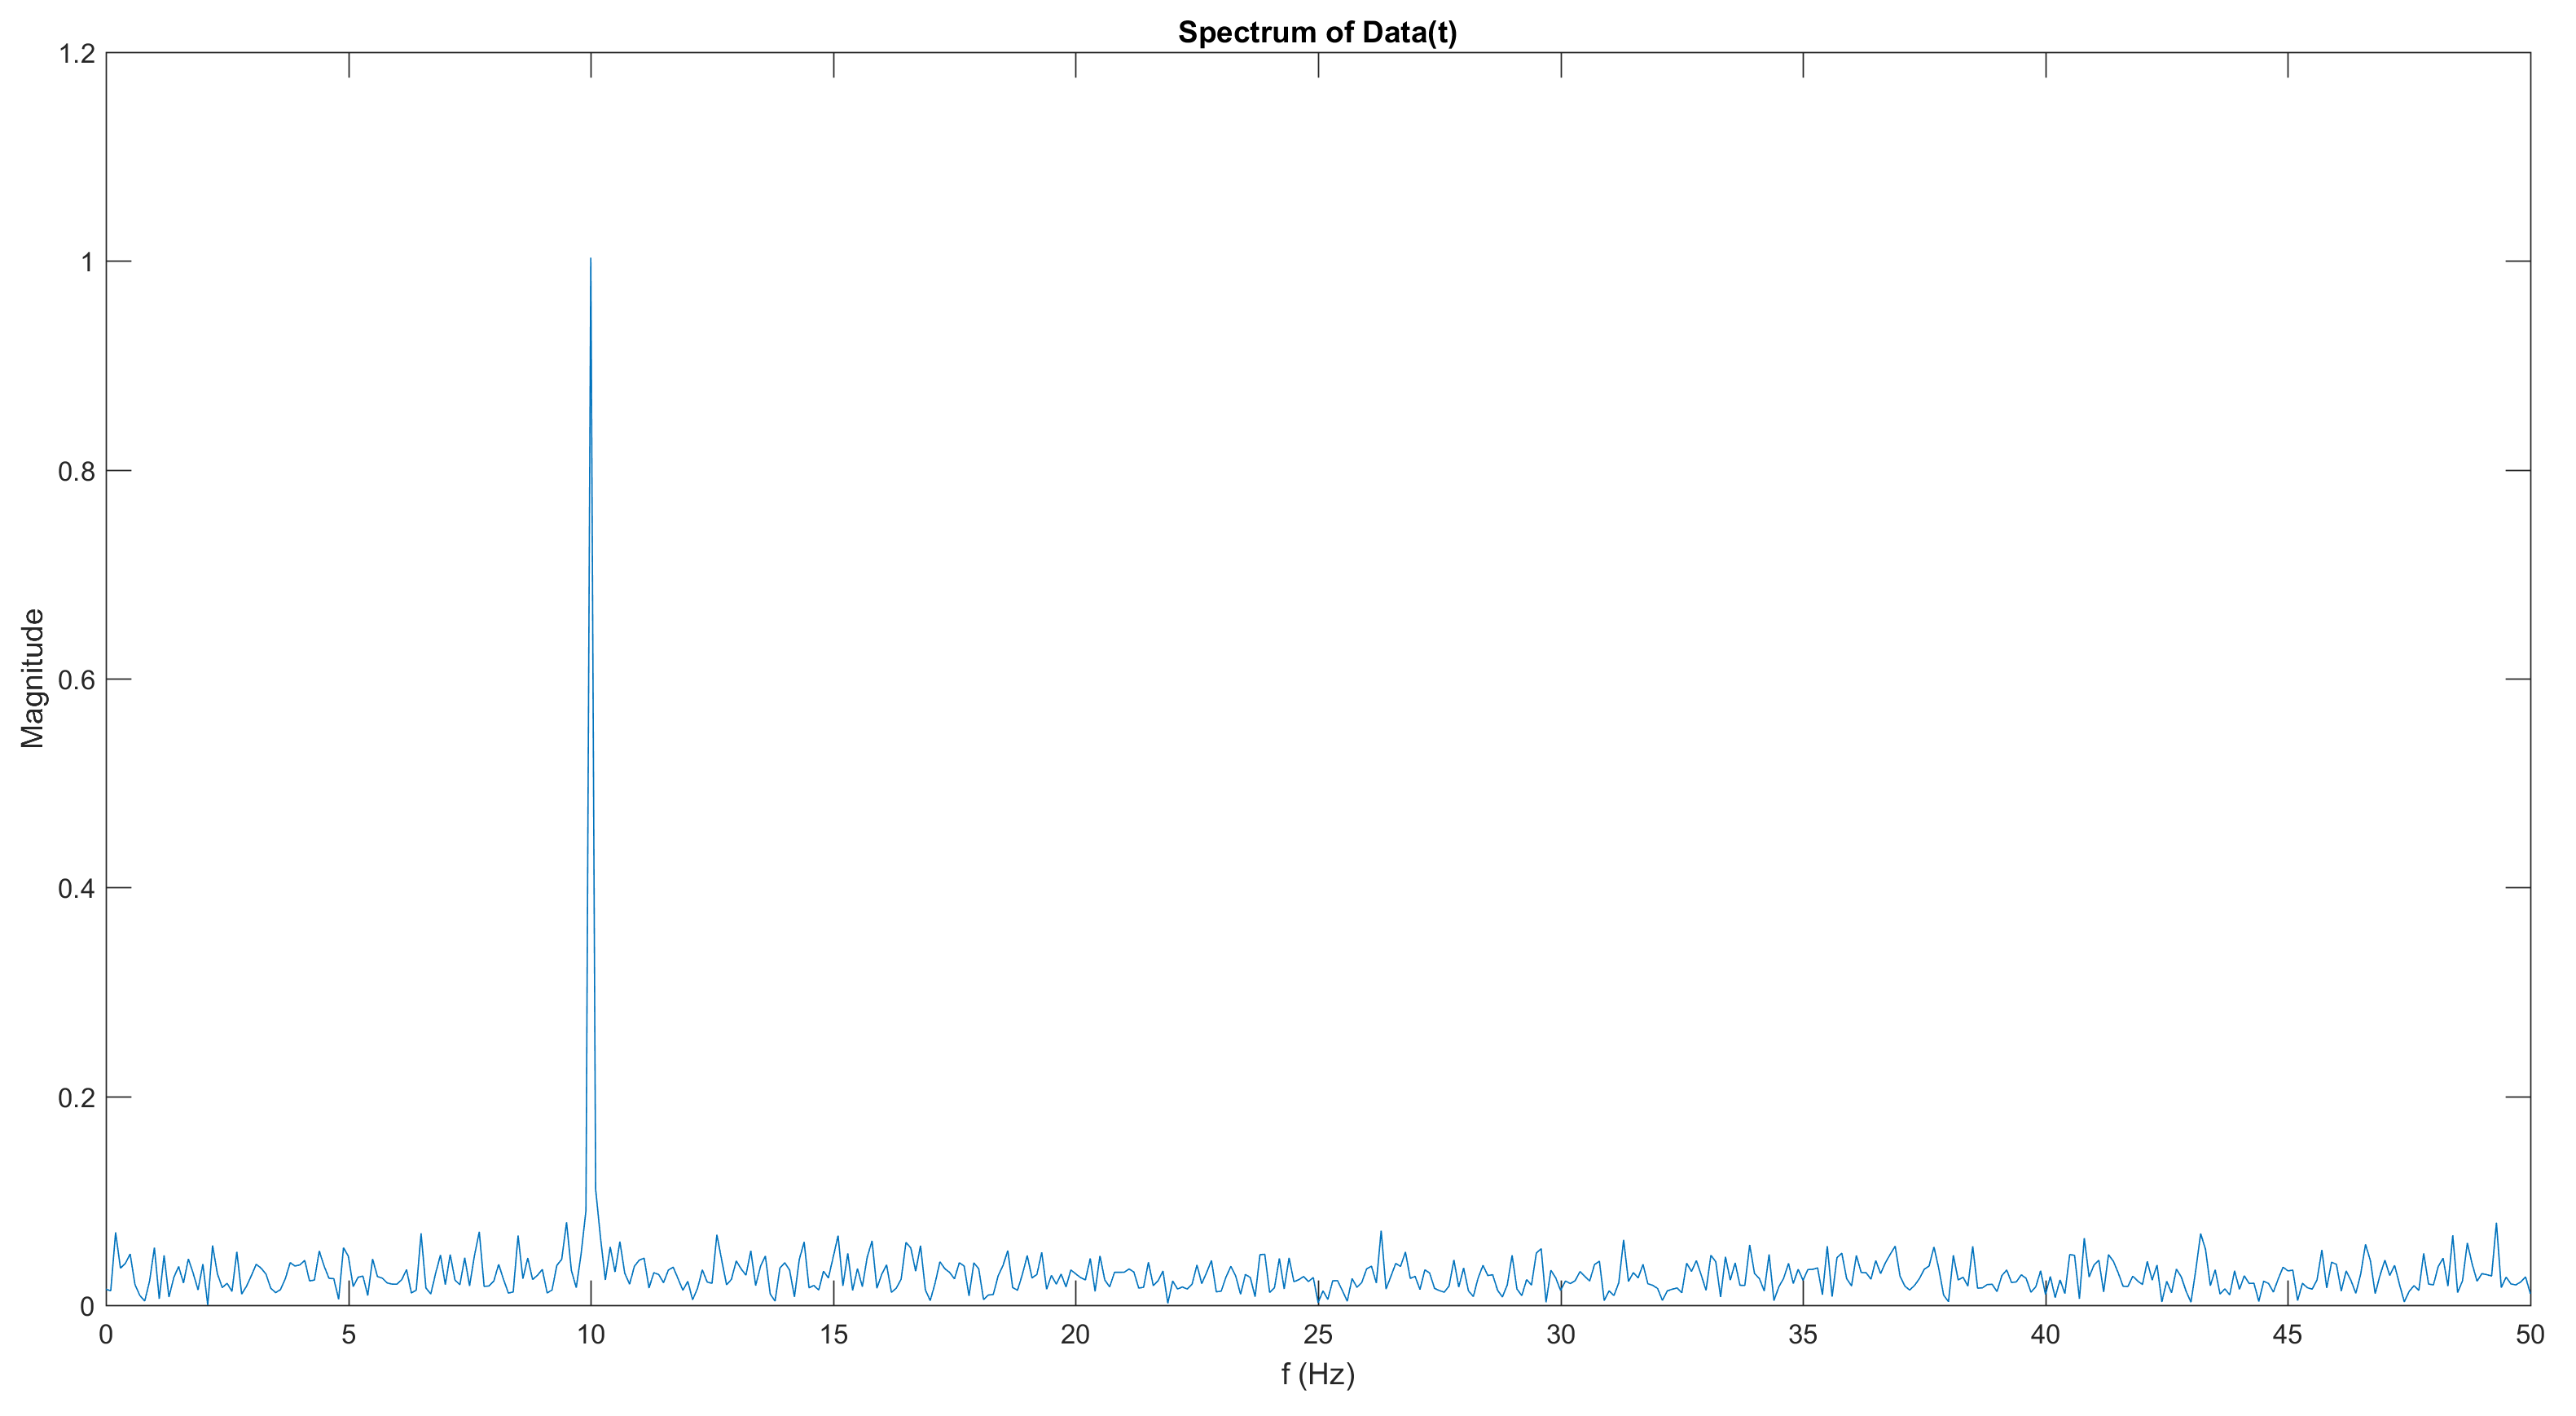
\includegraphics[scale=0.18]{fft}
\caption{Fast Fourier Transform}
\end{figure}\label{fig: Fast Fourier Transform}

It is possible see that there is a peak around $10 \thinspace Hz$. This frequency can be used like cutoffrequency to filtering out the noise, depends the filter you want to use, like Low Pass Filter\ref{ssc:Low Pass Filter}, or High Pass Filter\ref{ssc:High Pass Filter}.



\section{GPS points division} \label{sc:GPS points division}
Another problem to fix is the way geolocation points are identified.
As discussed in Chapter\ref{ch:Inertial Measurement Unit} , (GPS section\ref{pr:GPS}, on a page: \pageref{pr:GPS}), GPS records the data at a frequency of $1$ $Hz$ (every second), however, the acceleration data as we have seen in our case are recorded at $100$ $Hz$ (every $10$ $ms$). 
For every GPS recording, $100$ acceleration data will be registered. This puts us in front of a problem because if we want to map the road surface correctly, GPS data need to be very close to each other.
To understand better this factor, two different GPS coordinates were identified:

\begin{center}
 $Start = (Latitude_{start}, Longitude_{start})$\\
 $End = (Longitude_{end}, Longitude_{end})$
\end{center}

show on the figure below:
\begin{figure}[H]	
\centering
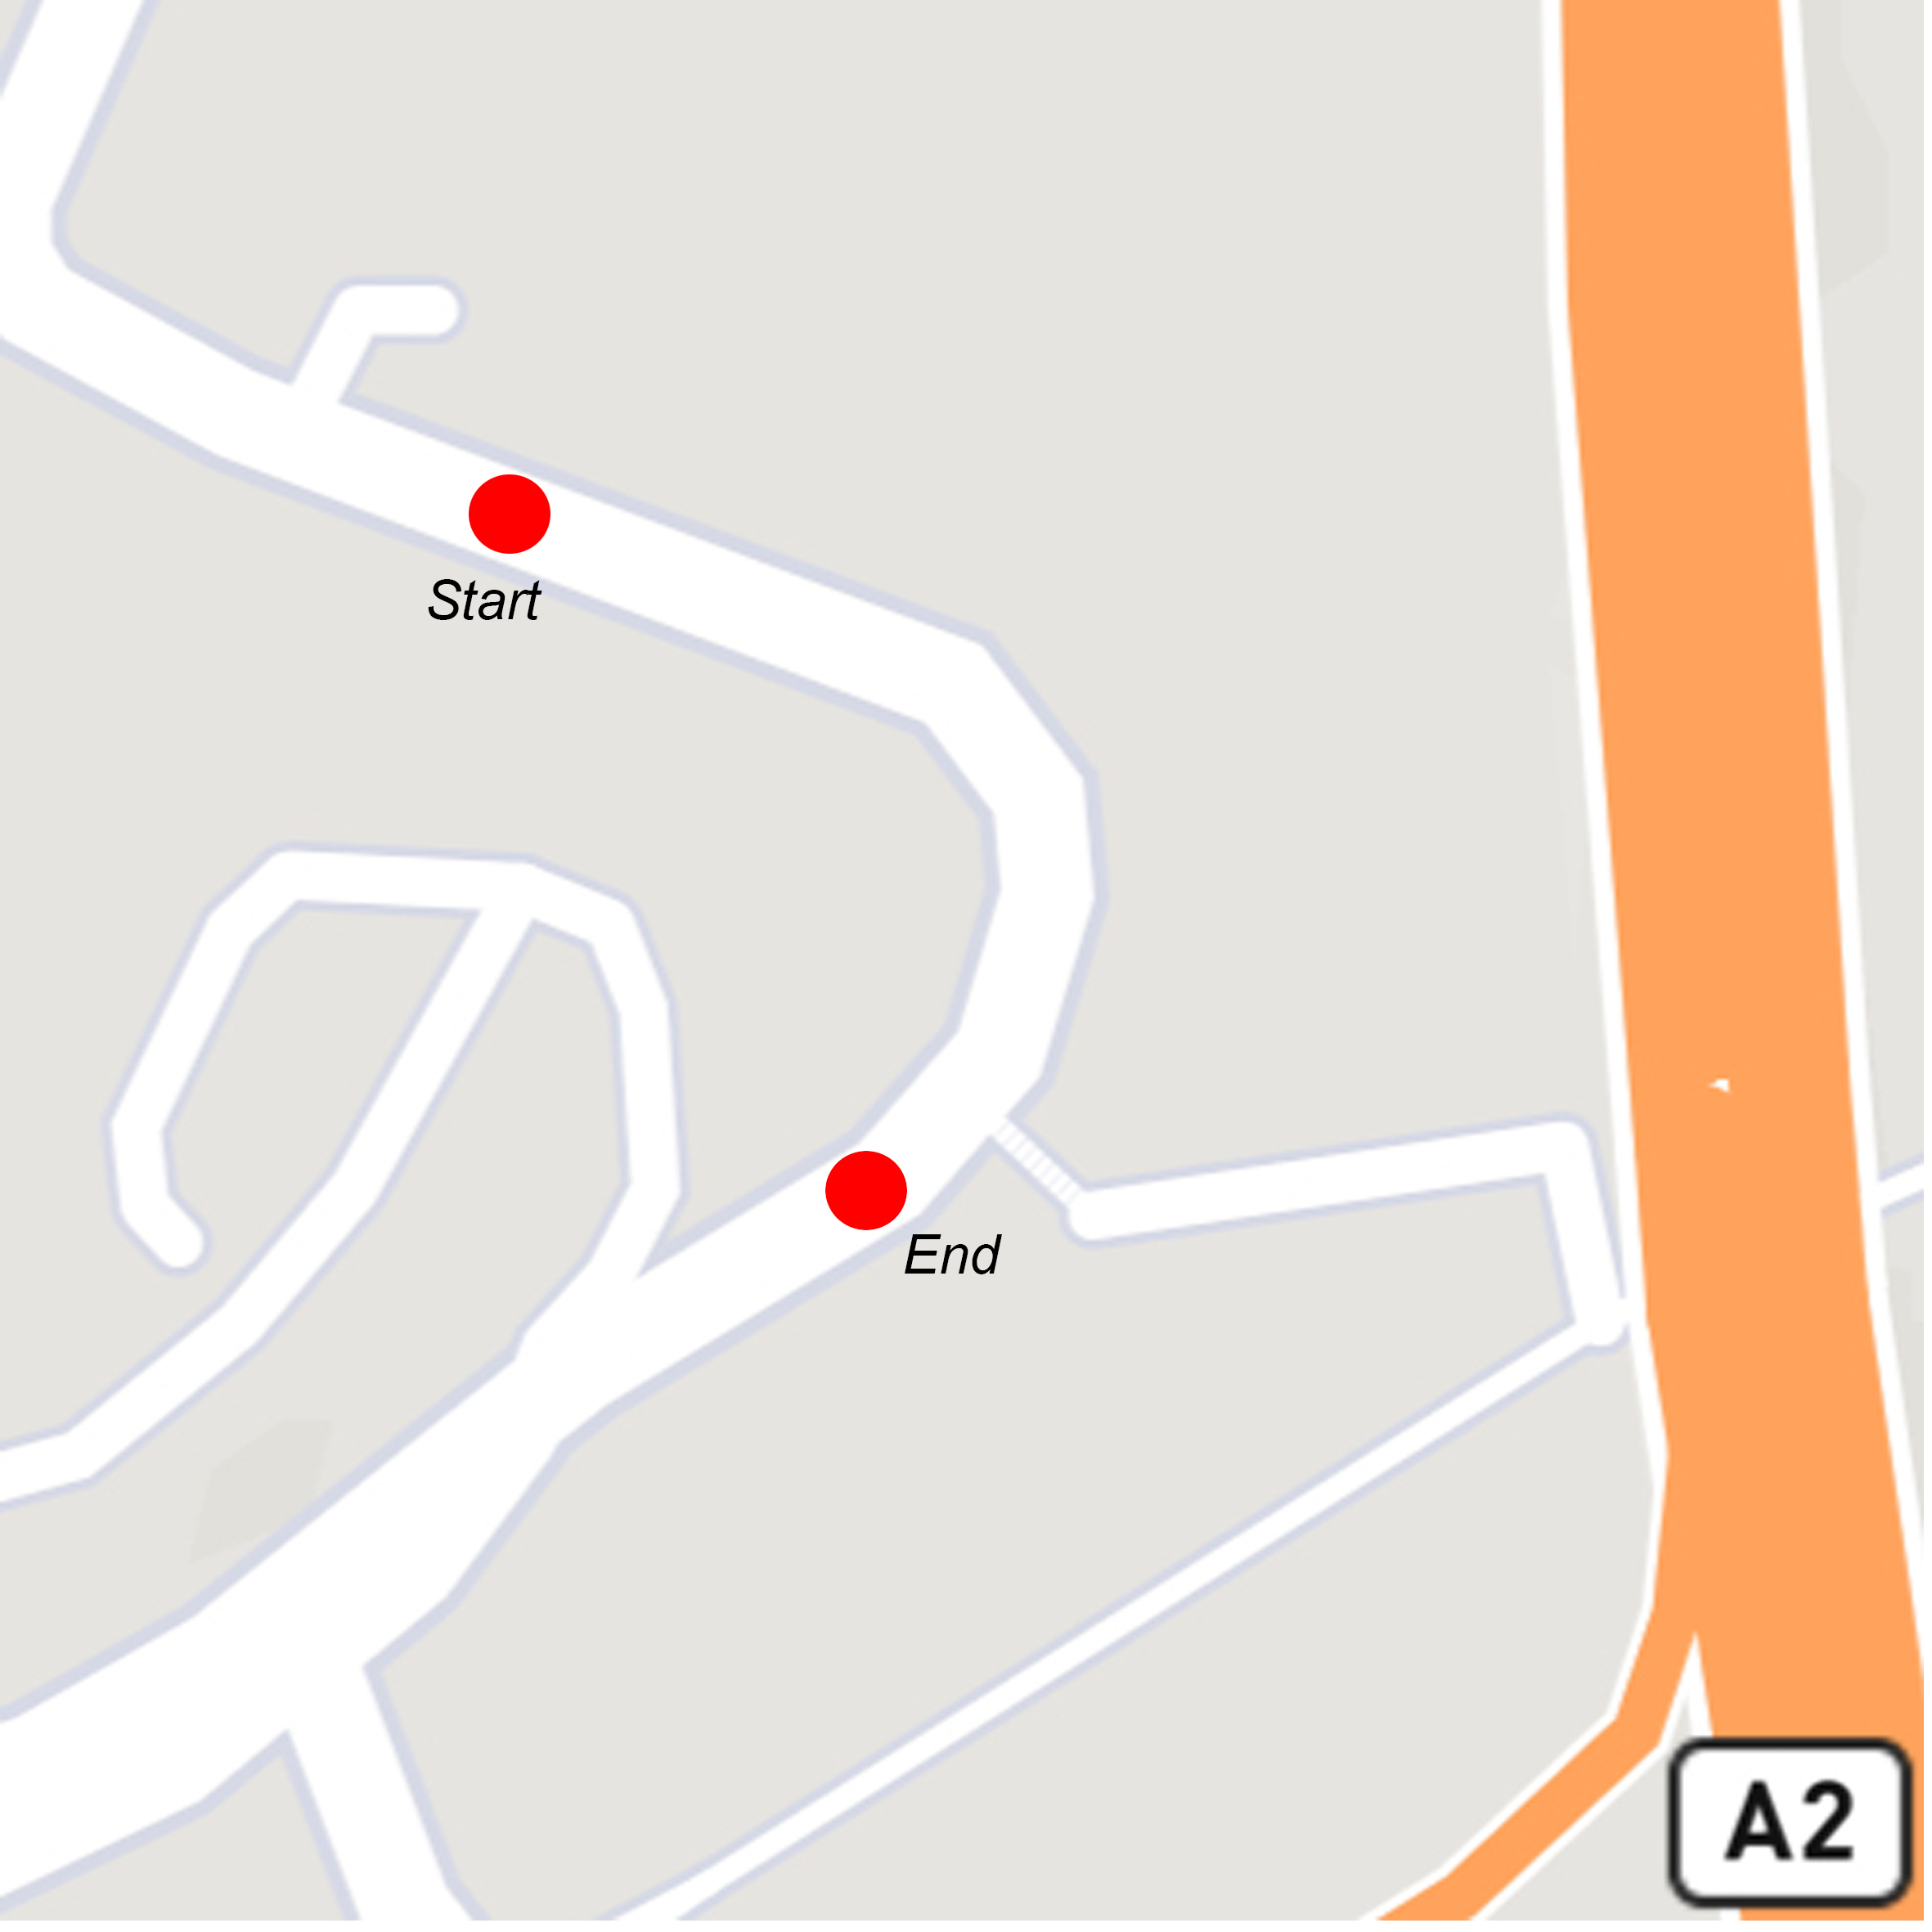
\includegraphics[scale=0.55]{Problem} \label{GPS Points Problem}
 \caption{Start and End points}
  \label{fig:GPS Points Problem}
\end{figure}


As we can see, we have two different GPS points, but we have a data accumulation at the $Start$ point, in our case equal to $100$ measurements and each of these has $Start$ point as GPS coordinate, the situation is analogue to the $End$ point.
Start point recordings refer to all $Start-End$ segment, but the intermediate coordinates of the segment are not recorded, and that is what is needed to properly locate the road surface conditions.
Therefore, a methodology has been developed, which from two different GPS points, allows determining the intermediate points in the segment. As shown in the Matlab code below.
\vspace{0.1cm}
\label{alg:Redefine Latitude And Longitude}
\lstset{language=Matlab}          % Set your language (you can change the language for each code-block optionally)
\begin{lstlisting}  % 
function [NewLatitude, NewLongitude] =
 redefineLatitudeAndLongitude (ReadedLatitude, ReadedLongitude)

NewLatitude = zeros(1, 1);
NewLongitude = zeros(1, 1);
i = 1;
    
for y = 2:numel(ReadedLongitude)    
  latlon1 = [ReadedLatitude(i,1), ReadedLongitude(i,1)];
  latlon2 = [ReadedLatitude(y,1), ReadedLongitude(y,1)];
  
  distance = lldistkm(latlon1,latlon2);   

    if(distance ~= 0)    
       LatitudeDifference = ReadedLatitude(y,1) - ReadedLatitude(i,1);
       LongitudineDifference = ReadedLongitude(y,1) - ReadedLongitude(i,1);
       steps = y - i;
   
       NewLongitude(i,1) = ReadedLongitude(i,1);
       LongitudeToAdd = LongitudineDifference / steps;
       for ix = i+1:y-1
        NewLongitude(ix,1) = NewLongitude(ix-1,1)+LongitudeToAdd;
       end       
       NewLongitude(y,1) = ReadedLongitude(y,1);
       
       NewLatitude(i,1) = ReadedLatitude(i,1);
       LatitudeToAdd = LatitudeDifference / steps;
       for ix = i+1:y-1
           NewLatitude(ix,1) = NewLatitude(ix-1,1)+LatitudeToAdd;
       end
       NewLatitude(y,1) = ReadedLatitude(y,1);   
    
    i = y;
    end
end 
\end{lstlisting}
\begin{center}
Code to divide the point inside a segment.
\end{center}
The proposed algorithm, when distinguishing two points having a distance between them different from $0$ $\si{\km}$, calculated by the \textit{haversine formula}\ref{ssc:Haversine Formula} that will be explained later, begins the definition of intermediate GPS points in the segment.
Beginning from the $Start$ point, until to the $End$ point, all intermediate points for both Latitude and Longitude will be calculated, as the previous point plus the difference in Latitude between the Start point and the End point, divided by the number of occurrences between Start and End, analogue procedure for Longitude.

Final result is shown in the figure:

\begin{figure}[H]	
\centering
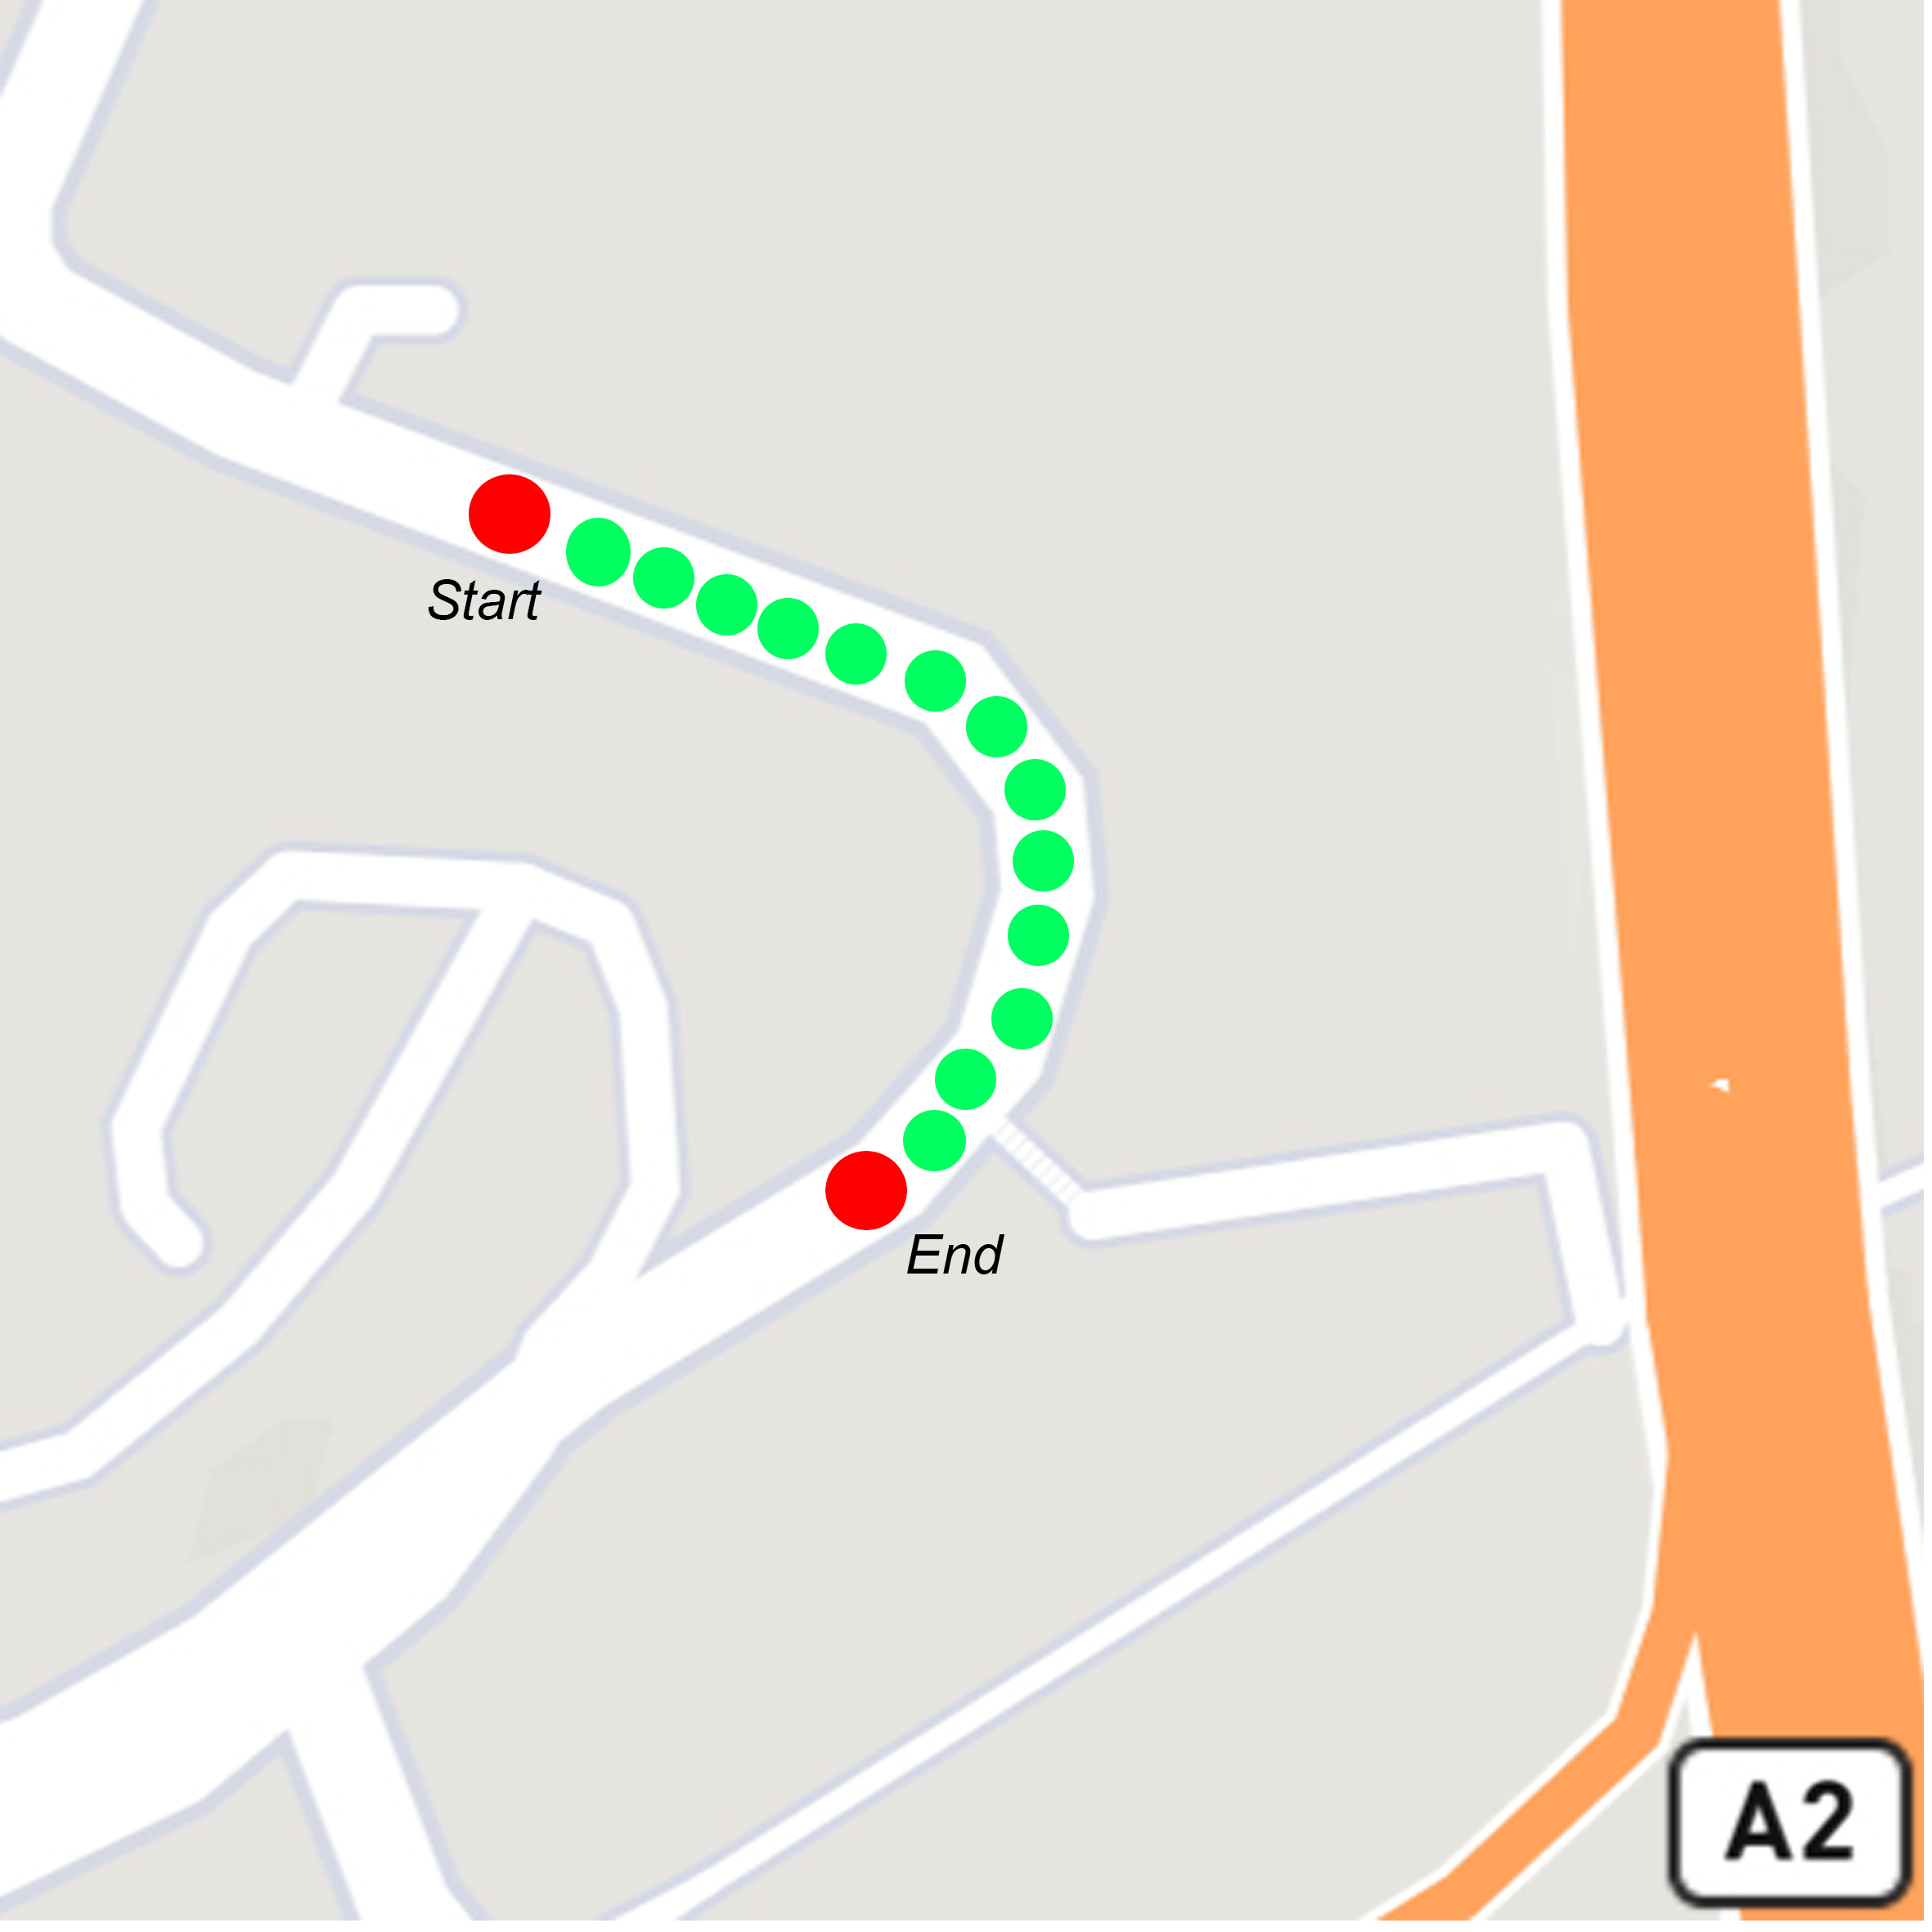
\includegraphics[scale=0.45]{ProblemSolved} \label{Solved GPS Points Problem}
 \caption{Start and End points}
  \label{fig:Solved GPS Points Problem}
\end{figure}

\subsection{Haversine Formula} \label{ssc:Haversine Formula}
This formula is particularly useful because it allows calculating the geographical distance between two points. Particularly in our case, it is mainly used for:
\begin{itemize}
\item Determine if there is a not null distance between two geographic points, so that the segment can be subdivided\ref{alg:Redefine Latitude And Longitude}.
\item Applied during the data processing, since following the subdivision, all consecutive geolocation points will have a very small distance.
For example, if we go at very low speeds, and take two consecutive points, their distance can be measured in the order of $cm$, otherwise, at very high speeds, the distance between the points are usually measured approximately in the order of a few $mt$.
The points to be correctly displayed on the map must be at a specified distance ($distance_{th}$) from each other.
It will be checked from an initial point $Start$, what are all the points that gradually adding their distances to each other, reaching $distance_{th}$, so a new point is created, and all those considered to arrive at $distance_{th}$ are eliminating (for acceleration values, however, different operations are performed depending on the index being calculated).This operation will be repeated for all points in the data set until we will have each point distant from each other by $distance_{th}$.
\end{itemize}

\noindent Haversine Formula calculates geographic distance on earth. Given two different latitude – longitude values of two different point on earth, then with the help of Haversine Formula, it is easily possible compute the great-circle distance (The shortest distance between two points on the surface of a Sphere). 		
\noindent The haversine formula is defined like follow:

\noindent Given two points:
\begin{center}
$Start$ = ($\phi_{1} , \lambda_{1}$)\\
$End$ = ($\phi_{2} , \lambda_{2}$)
\end{center}

where:
\begin{itemize}
\item $\phi$ represent the $Latitude$.
\item $\lambda$ the $Longitude$.
\item $r$ is the radius of the earth.
\item $d$ the distance between the two points.
\end{itemize} 
\begin{center}
$ hav \thinspace \left(\dfrac{d}{r}\right) = \thinspace hav \thinspace (\phi_{2} - \phi_{1}) \thinspace + \thinspace \cos (\phi_{1}) \thinspace \cos(\phi_{2}) \thinspace hav(\lambda_{2} - \lambda_{1})$
\end{center}
$hav$ is the haversine function defined:

\begin{center}
$hav(\theta) = \sin^{2} \left(\dfrac{\theta}{2}\right)$
\end{center}

The sign $\dfrac{d}{r}$ is the central angle, assuming angles are measured in radians (note that $\phi$ and $\lambda$; can be converted from radians to degrees by multiplying by $\left(\dfrac{180}{\pi}\right)$).
Solve for d by applying the inverse haversine (if available) or by using the arcsine (inverse sine) function, the distance is calculated like follow:

\begin{center}
 $d = 2r \thinspace \arcsin \thinspace \left(\sqrt{\sin^{2} \left(\dfrac{\phi_{2} - \phi_{1}}{2}\right) \thinspace + \thinspace \cos (\phi_{1}) \thinspace \cos(\phi_{2}) \thinspace \sin^{2} \left(\dfrac{\phi_{2} - \phi_{1}}{2}\right) }\right) $
\end{center}
The distance result is can represent in $km, mt, ...$ depending on the unit misure of $r$.

The figure below shown an example of application of Haversine Formula, to calculate flying distance from Universita' della Calabria to Cosenza.

\begin{figure}[H]	
\centering
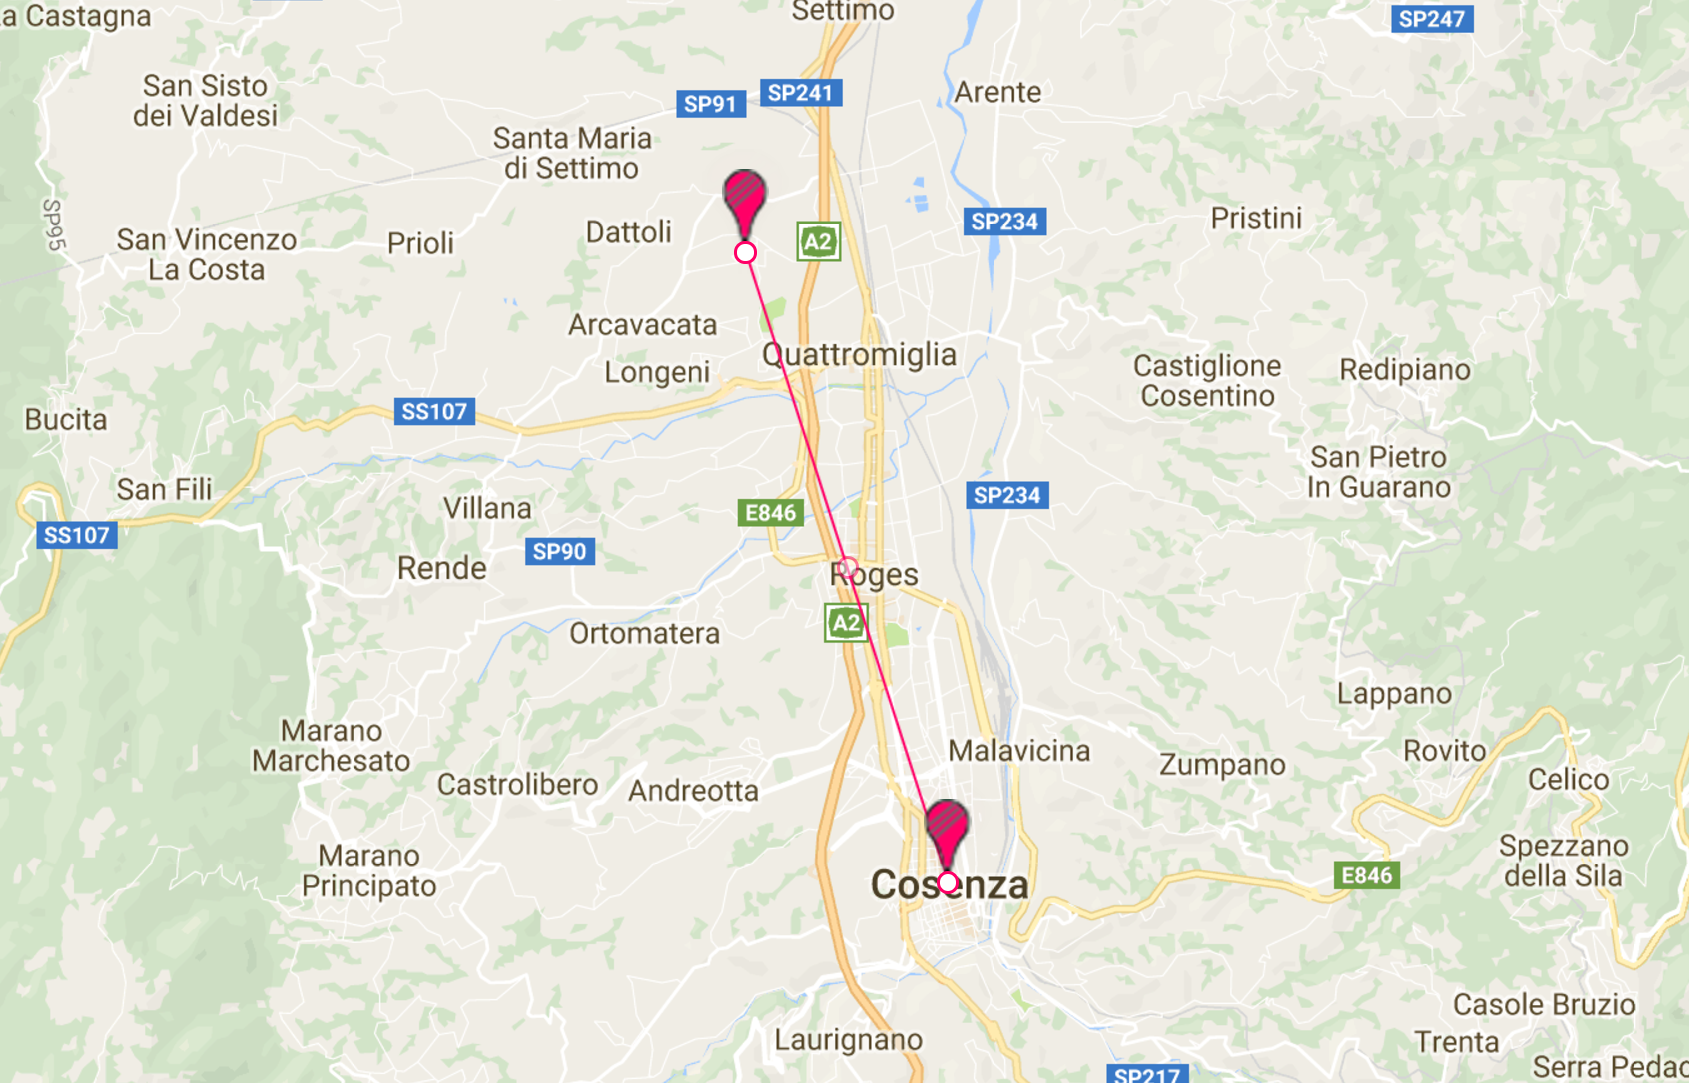
\includegraphics[scale=0.75]{Haversine} 
\\In this example the flying distance is $7.13 \thinspace \si{km}$
 \caption{Haversine Example}
  \label{fig:Haversine Example}
\end{figure}
\end{document}



